% !TeX encoding = UTF-8
% 此文件从2022.7开始

\chapter{子流形}\label{chsm}
\S \ref{chdm:sec_sub-manifold}已经初步讨论了子流形概念;
在引入度规后,可研究的子流形内容更加丰富.
我们先给出子流形的一般理论,然后再把这些理论应用到超曲面上;
超曲面在广义相对论中有重要应用.
需要声明的是:除非显示标注“零模”,否则所有内容只适用于非零模理论,
包括曲线、曲面、子流形等等.


设有两个广义黎曼流形$M$和$N$,维数分别为$m$和$n(<m)$,
假设存在光滑\uwave{浸入映射}$\phi:N\to M$,%(证明存在性是个艰难的课题)
即切映射$\phi_{*}$处处非退化;
$M$和$N$的局部坐标分别为$(V;x^\alpha)$和$(U;y^i)$,且$\phi(U)\subset V$.
指定$g_{ab}$是流形$M$的广义黎曼度规.
第\pageref{chdm:def_pullback-1form-onfield}页的定义\ref{chdm:def_pullback-1form-onfield}指出
拉回张量$h_{ab}\equiv\phi^{*}g_{ab}$也是流形$N$上的张量场,容易验证$h_{ab}$也是对称的;下面证明
它还是非退化的.与式\eqref{chrg:eqn_isometry-MNcoord}推导过程完全相同,可得
\begin{equation}\label{chsm:eqn_gijhab}
    h_{ij}= h_{ab} \left(\frac{\partial }{\partial y^i}\right)^a
    \left(\frac{\partial }{\partial y^j}\right)^b = \frac{\partial x^\alpha}{\partial y^i}
    \frac{\partial x^\beta}{\partial y^j} g_{\alpha\beta} .
\end{equation}
注意,此时的Jacobi矩阵$\frac{\partial x^\alpha}{\partial y^i}$不是方阵.上式
等号最右端是三个矩阵相乘,它们都是非退化矩阵,所以乘积之后的秩是$\min(m,n)$,即
矩阵$h_{ij}$的秩是$n$;因此$h_{ij}$是非退化的.虽然上面是从分量角度来论证的,但是
基矢是任选的,而且矩阵的秩不随基矢改变而改变;最终可知二阶对称张量场$h_{ab}$是非退化的.

此时,把二阶、对称、非退化张量场$h_{ab}\equiv\phi^{*}g_{ab}$称为广义黎曼流形$M$中度规$g_{ab}$通过
映射$\phi$拉回到流形$N$上的{\heiti 诱导度规}.
在古典微分几何中,称度规为第一基本形式;我们称诱导度规$h_{ab}$为子流形$N$的{\heiti 第一基本形式}.

需要强调的是流形$N$中原来可能存在另外一个度规场,但我们只用诱导度规\eqref{chsm:eqn_gijhab};
也就是我们只考虑等距浸入,不考虑非等距情形.

当$m=n+1$时,流形$N$称为$M$的浸入超曲面.
%为给读者初步认知,下面讨论两个简单例子,在后面会进一步讨论这个话题.




\section{子流形基本理论}
设$(M,g,\nabla_a)$是$m$维广义黎曼流形,$(N,h,{\rm D}_a)$是$n(<m)$维广义黎曼流形.
假设两个流形间存在光滑\uwave{局部等距浸入}映射$\phi:N \to M$,
局部等距即是$h_{ab}=\phi^* {g}_{ab}$.
$\forall p\in N$,存在该点开邻域$p \in {U}\subset N$使
得$\phi|_{U}: {U}\to {V}\subset {M}$是\uwave{等距、正则嵌入}映射;
因此,在局部上$(\phi,N)$是正则嵌入的;正因为如此,在局部上通常用包含映射$\imath$来代替
前面给出的浸入映射$\phi$,即$\imath:{U}\to {V}$或$\imath:N \to {M}$(应理解成只在局部成立).
我们常常把$N$和$\imath(N)$等同起来,把$T_pN$和$\imath_* (T_p N)$也看作认同,等等.
同时,很多时候会忽略$\phi_{*},\phi^{*}$,$\imath_*,\imath^*$等记号;
绝大部分文献皆如此,我们也无意改变这种记号习惯,读者小心理解、区分便是,只是在
笔者认为需要强调的时候会恢复省略的记号.


$\forall p\in N$,切空间$T_{\imath(p)} M$关于广义黎曼度规${g}_{ab}$可以分解为\uwave{正交直和}
\begin{equation}
    T_{\imath(p)}{M} = T_pN \oplus T_p^\bot N ,
\end{equation}
其中$T_pN$是$N$在$p$点的切空间(用正则嵌入映射将之
与$\imath_* (T_pN)\subset T_{\imath(p)}{M}$等同),
因此可把$T_pN$看作$T_{\imath(p)} M $的子空间;
$T_p^\bot N$是$T_pN$在$T_{\imath(p)}{M}$中的正交补空间,即
\begin{equation}\label{chsm:eqn_orthogonal-decomposition-TN-TbN}
    T_p^\bot N=\bigl\{ \xi^a \in T_{\imath(p)}{M}\ |\
    {g}_{ab}\xi^a v^b=0,\ \forall v^b\in T_pN \bigr\} ,
\end{equation}
称为子流形$\imath : N\to {M}$在点$\imath(p)$的{\heiti 法空间};
法空间的维数$m-n$称为{\heiti 余维数}.
这样,$\forall v^a\in T_p{M}$可唯一分解为
\begin{equation}\label{chsm:eqn_orthogonal-decomposition}
    v^a = {}^\top v^{a} + {}^\bot v {^a} ,
\end{equation}
其中${}^\top v^{a} \in T_pN$称为切分量(Tangent),
${}^\bot v {^a} \in T_p^\bot N$称为法分量(Normal).令
\begin{equation}
    T^\bot N = \bigcup_{p\in N} T_p^\bot N ,
\end{equation}
可以证明$T^\bot N$是流形${M}$上的一个矢量丛,
称为子流形$\imath : N\to {M}$的{\heiti 法丛}.
需注意,法空间、法丛中所有矢量属于$T_{\imath(p)}{M}$,
并且不属于$T_pN$($\equiv\imath_*(T_pN)$)的矢量.
\uwave{用$\mathfrak{X}^\bot (N)$}表示法丛$T^\bot(N)$中的可微截面集合,
即法向矢量场集合.

需假设法丛中没有零模矢量;在第\ref{chnull}章会初步涉及零模法矢量的内容.


\index[physwords]{子流形联络}
\index[physwords]{联络!子流形联络}

\subsection{子流形联络}
设${\nabla}_a$是黎曼流形$({M},{g})$的Levi-Civita联络.
$\forall X^a, Y^a \in \mathfrak{X}(N)$,
$\imath_* X^a, \imath_* Y^a$是${M}$中
沿$\imath$的切矢量;为使意义清晰,我们将多次写出“$\imath_*$”等记号.
显然${\nabla}_{\imath_* X} (\imath_* Y^a) \in \mathfrak{X}({M})$,
但它未必是$\imath_* (\mathfrak{X}(N)) \subset \mathfrak{X}({M})$中的切矢量;
利用式\eqref{chsm:eqn_orthogonal-decomposition},可以假设 %(省略“$\imath_*$”)
\begin{equation}\label{chsm:eqn_Gauss}
    {\nabla}_{\imath_* X} (\imath_*Y^a) = {\rm D}_{\imath_*X} (\imath_*Y^a)
    + K^a_{bc}  (\imath_*X^b, \imath_*Y^c),
\end{equation}
其中${\rm D}_{\imath_*X} (\imath_*Y^a)  = {}^{\top}({\nabla}_{\imath_* X} (\imath_*Y^a))$,
那么$ {\rm D}_{\imath_*X} (\imath_*Y^a) \in \imath_* (\mathfrak{X}(N))\equiv \mathfrak{X}(N) $,
所以通常会把${\rm D}_{\imath_*X} (\imath_*Y^a) $简记为${\rm D}_{X} Y^a $;
另一部分$K^a_{bc}(\imath_*X^b,\imath_*Y^c) = {}^{\bot}({\nabla}_{\imath_* X} (\imath_*Y^a)) $,
是法丛$T^\bot N$中的矢量,在不引起误解的前提下也简记为$K^a_{bc} (X^b ,Y^c)$.
式\eqref{chsm:eqn_Gauss}通常称为{\bfseries\heiti Gauss公式};
$K^a_{bc}$称为等距浸入$\imath$的{\heiti 第二基本形式},
或称为$N$在${M}$中的第二基本形式.

我们需要证明上式中给出${\rm D}_a$是流形$(N,h)$中的Levi-Civita联络.




\begin{theorem}\label{chsm:thm_Dg}
    设$\imath:N\to M$为局部等距浸入,$(M,g)$上有Levi-Civita联络$\nabla_a$;
    则式\eqref{chsm:eqn_Gauss}中的${\rm D}_a$是流形$(N,h)$中的Levi-Civita联络.
\end{theorem}
\begin{proof}
    先验证线性.$\forall f\in C^\infty(N)$、$\forall X^a,Y^a,Z^a\in TN$,
    取${\nabla}_{X} (Y^a+fZ^a)$的切向和法向:
    \begin{align*}
        {\rm D}_{X}& (Y^a+f Z^a)={}^{\top}\bigl({\nabla}_{X} (Y^a+f Z^a)\bigr) 
        ={}^{\top}\bigl({\nabla}_{X} (Y^a)+X(f)Z^a+f {\nabla}_{X} (Z^a)\bigr) \\
        =&{}^{\top}\bigl({\nabla}_{X} (Y^a) \bigr)+{}^{\top}\bigl(X(f)Z^a+f {\nabla}_{X} (Z^a)\bigr)  
        = {\rm D}_{X} (Y^a)+\bigl(X(f)Z^a +f {\rm D}_{X} (Z^a)\bigr). \\
        K^a_{bc} &(X^b,Y^c+f Z^c)={}^{\bot}\bigl({\nabla}_{X} (Y^a+fZ^a)\bigr) 
        ={}^{\bot}\bigl({\nabla}_{X} (Y^a)+X(f)Z^a+f{\nabla}_{X} (Z^a)\bigr) \\
        =& {}^{\bot}\bigl({\nabla}_{X} (Y^a)\bigr)
        +{}^{\bot}\bigl(f{\nabla}_{X} (Z^a)\bigr)
        = K^a_{bc} (X^b,Y^c)+f K^a_{bc} (X^b,Z^c).
    \end{align*}
    接着验证加法:
    \begin{align*}
        {\rm D}_{X+fY} Z^a=&{}^{\top}\bigl({\nabla}_{X+fY} Z^a\bigr) 
        ={}^{\top}\bigl({\nabla}_{X} Z^a+{\nabla}_{fY} Z^a\bigr) \\
        =&{}^{\top}\bigl({\nabla}_{X} Z^a\bigr)+f{}^{\top}\bigl({\nabla}_{Y} Z^a\bigr)
        ={\rm D}_{X} Z^a + f{\rm D}_{Y} Z^a . \\
        K^a_{bc} (X^b+fY^b, Z^c)=&{}^{\bot}\bigl({\nabla}_{X+fY} Z^a\bigr) 
        ={}^{\bot}\bigl({\nabla}_{X} Z^a+{\nabla}_{fY} Z^a\bigr) \\
        =&{}^{\bot}\bigl({\nabla}_{X} Z^a\bigr)+f{}^{\bot}\bigl({\nabla}_{Y} Z^a\bigr)
        =K^a_{bc} (X^b, Z^c)+f K^a_{bc} (Y^b, Z^c) .
    \end{align*}
    上面几个式子说明${\rm D}_X$符合$N$上\uwave{仿射联络}定义;
    同时,验证了$K^a_{bc} (\cdot, \cdot)$对每个位置均是$C^\infty(N)$-线性.

    此外,仍需证明它是无挠性、相容性.我们已知联络${\nabla}_a$是无挠的,即有
    \begin{equation}
    \begin{aligned}
        0=&{\nabla}_{X} Y^a - {\nabla}_{Y} X^a -[{X}, {Y}]^a \\
         =&{\rm D}_{X} Y^a - {\rm D}_{Y} X^a -[X, Y]^a + K^a_{bc} (X^b ,Y^c) -K^a_{bc} (X^c, Y^b) .
    \end{aligned}
    \end{equation}
    需注意$[{X}, {Y}]^a=[\imath_*X, \imath_*Y]^a  =\imath_* ([X,Y]^a)$,
    显然已把$\imath_* ([X,Y]^a)$和$[X,Y]^a$作认同;读者需注意
    $[X,Y]^a\in \mathfrak{X}(N)$,推前之后的$\imath_* ([X,Y]^a)\in \imath_*\mathfrak{X}(N)$,
    推前映射是不会把切矢量“推出”法空间分量的.
    对上式分别取切向部分和法向部分,有
    \begin{align}
        0=& {\rm D}_{X} Y^a - {\rm D}_{Y} X^a -[X, Y]^a, \label{chsm:eqn_tmp-tan22} \\
        0=& K^a_{bc} (X^b, Y^c) -K^a_{bc} (X^c, Y^b). \label{chsm:eqn_tmp-nor22}
    \end{align}
    由式\eqref{chsm:eqn_tmp-tan22}可知,仿射联络${\rm D}_a$是无挠的.

    将$X^a\in \mathfrak{X}(N)$作用在标量场上,有(其中$Y^a,Z^a\in \mathfrak{X}(N)$)
    \begin{equation}\label{chsm:eqn_tmptn50}
         {X}({h}_{bc} {Y}^b {Z}^c) ={X}\bigl((\imath^*g_{bc}) {Y}^b {Z}^c \bigr)
         = {X}\bigl(g_{bc} (\imath_* {Y}^b) (\imath_*{Z}^c) \bigr)
         =X(g_{bc} Y^b Z^c)
    \end{equation}
    我们已知联络${\nabla}_a$是与${g}_{ab}$相容的,即有
    \begin{align*}
        {X}({g}_{bc} {Y}^b {Z}^c) =&  {g}_{bc} ({\nabla}_{X} {Y}^b ){Z}^c +{g}_{bc} {Y}^b {\nabla}_{X}{Z}^c \\
       =& {g}_{bc}{Z}^c {\rm D}_{X} Y^b  +{g}_{bc}{Z}^c  K^b_{ad} (X^a, Y^d)
         +{g}_{bc}{Y}^b {\rm D}_{X} Z^c  +{g}_{bc}{Y}^b  K^c_{ad} (X^a, Z^d)
    \end{align*}
    注意到${Z}^c$是切矢量部分,而$K^b_{ad} (X^a, Y^d)$是法矢量部分,故两者内积必然为零.
    继续计算,有(注意$\imath_*({\rm D}_{X} Y^b) ={\rm D}_{X} Y^b$)
    \setlength{\mathindent}{0em}
    \begin{equation}\label{chsm:eqn_tmptn60}
    \begin{aligned}
        &X(h_{bc} Y^b Z^c)\xlongequal{\ref{chsm:eqn_tmptn50}} {X}({g}_{bc} {Y}^b {Z}^c)=
        {g}_{bc}\imath_* ({Z}^c {\rm D}_{X} Y^b)  +{g}_{bc}\imath_*({Y}^b {\rm D}_{X} Z^c ) \\
        =&\imath^*({g}_{bc})({Z}^c {\rm D}_{X} Y^b)+\imath^*({g}_{bc})({Y}^b {\rm D}_{X} Z^c )
        = h_{bc}{Z}^c {\rm D}_{X} Y^b+ h_{bc} Y^b {\rm D}_{X} Z^c  .
    \end{aligned}
    \end{equation}\setlength{\mathindent}{2em}
    因此联络与度规相容,所以${\rm D}_a$是流形$N$的Levi-Civita联络.
\end{proof}

不难得到对偶矢量场的协变导数公式,与式\eqref{chsm:eqn_Gauss}相对应:
\begin{equation}\label{chsm:eqn_Gauss-dualvector}
    {\nabla}_{X} {\omega}_a = {\rm D}_{X} {\omega}_a - K^c_{ba}{X}^b {\omega}_c;
    \quad {\text{其中}}\ \forall {\omega}_a \in \mathfrak{X}^*(N),
    \quad \forall X\in \mathfrak{X}(N).
\end{equation}


此后,当不引起混淆时,把$K^b_{ad} (X^a, Y^d)$记成$K^b_{ad} X^a Y^d$.
由上面定理的证明过程(例如式\eqref{chsm:eqn_tmp-nor22})可得
关于$K: \mathfrak{X}(N)\times \mathfrak{X}(N) \to \mathfrak{X}^\bot(N)$的如下命题:
\begin{proposition}\label{chsm:thm_hII}
    映射$K$是
    对称的($K^a_{bc}=K^a_{cb}$)、$C^\infty(N)$-双线性的.
\end{proposition}

\index[physwords]{法联络}

\subsection{法联络}
设$X^a\in \mathfrak{X}(N),\ {\xi}^a \in \mathfrak{X}^\bot(N)$,
可把${\nabla}_{X} \xi^a$分成切向、法向两部分
\begin{equation}\label{chsm:eqn_Weingarten}
    {\nabla}_{X} \xi^a = - S^a_{\xi b} X^b + {\rm D}_{X} ^\bot \xi^a .
\end{equation}
其中$S^a_{\xi b} X^b $和${\rm D}_{X} ^\bot \xi^a$
分别表示${\nabla}_{X} \xi^a$的切向和法向部分.
%绝大部分文献将$S^a_{\xi b} X^b$记成$S_{\xi} (X)$,这里增加了抽象指标记号.
公式\eqref{chsm:eqn_Weingarten}一般称为{\heiti \bfseries Weingarten 公式},
它和Gauss公式合称为{\heiti 子流形基本公式}.

参考定理\ref{chsm:thm_Dg}的证明过程,
可知式\eqref{chsm:eqn_Weingarten}中定义的${\rm D}_{X}^\bot$是一个\uwave{仿射联络},
称为流形$N$上的{\heiti 法联络};此映射是
${\rm D}_a ^\bot: \mathfrak{X}(M)\times
\mathfrak{X}^\bot(N)\to \mathfrak{X}^\bot(N)$.

$\forall \xi^a, {\eta}^a \in \mathfrak{X}^\bot(N)$,考虑到法向矢量与切向矢量内积恒为零,有
\begin{equation*}
    {g}_{ab} ({\rm D}_{X}^\bot \xi^a) {\eta}^b
    + {g}_{ab} \xi^a {\rm D}_{X}^\bot {\eta}^b
      \xlongequal{\ref{chsm:eqn_Weingarten}}
    {g}_{ab} ({\nabla}_{X} \xi^a) {\eta}^b
    + {g}_{ab} \xi^a {\nabla}_{X} {\eta}^b
    =X({g}_{ab} \xi^a {\eta}^b) .
\end{equation*}
上式说明法联络${\rm D}_{X}^\bot$与${g}$在法空间的诱导度规是相容的.
因为${\rm D}_{X}^\bot\xi^a$中的$X^a$和$\xi^a$分别属于切空间和法空间,
所以法联络${\rm D}_{a}^\bot$的无挠性不好探讨.


参考定理\ref{chsm:thm_Dg}的证明过程,可得如下命题:
\begin{proposition}\label{chsm:thm_Swein}
    由$(X,\xi)\xlongrightarrow{S}- S^a_{\xi b}(X^b)$定义的
    映射$S:\mathfrak{X}^\bot(N)\times \mathfrak{X}(N) \to \mathfrak{X}(N)$是
    $C^\infty(N)$-双线性的.一般称映射$S$为{\heiti 形状因子}.
\end{proposition}
因$S^a_{\xi b} : \mathfrak{X}(N) \to \mathfrak{X}(N)$,
故从张量场特征引理\ref{chdm:thm_Tensor-Characterization-Lemma-1}可知$S^a_{\xi b}$是
$N$上的$(1,1)$型光滑张量场;但因$\xi^a \in \mathfrak{X}^\bot (N)$,
故$S$(及$K$)不是流形$N$上的$(1,2)$型张量场.
但$S$和$K$却是流形${M}$上的$(1,2)$型张量场.

$\forall \xi^a \in \mathfrak{X}^\bot(N),
\ \forall X^a, Y^a \in \mathfrak{X}(N)$,
注意${g}_{ab} Y^a \xi^b=0$,有
\begin{align*}
    0={\nabla}_{X} ({g}_{ab} Y^a \xi^b)=
    {g}_{ab} Y^a {\nabla}_{X} \xi^b+
    {g}_{ab} {\nabla}_{X} ( Y^a ) \xi^b
    ={g}_{ab} K^a_{cd} X^c Y^d \xi^b
    -{g}_{ab} Y^a S^b_{\xi c} X^c .
\end{align*}
由上式及命题{\ref{chsm:thm_hII}}可得
\begin{equation}\label{chsm:eqn_sym-Sh}
    {g}_{ab} Y^a  S^b_{\xi c} X^c=
    {g}_{ab} K^a_{cd} X^c Y^d \xi^b
    ={g}_{ab} K^a_{dc}  Y^d X^c \xi^b
    ={g}_{ab} X^a S^b_{\xi c} Y^c .
\end{equation}
故,映射$S^a_{\xi b}:T_pN \to T_pN$关于
内积${g}_{ab}$是\uwave{对称线性变换}.
%用\S \ref{chmla:sec_tensor}记号表示此对称性为:
%\begin{equation}
%    \left< S_{\xi}(X), Y \right>
%  = \left< K(X,Y), \xi \right>
%  = \left< K(Y,X), \xi \right>
%   =\left< S_{\xi}(Y),X \right>  .
%\end{equation}


\subsection{子流形基本方程}
令${}^{m}R^d_{cab}$表示$m$维流形$M$中黎曼张量.
\begin{subequations}\label{chsm:eqn_riemann-MN-TN}
\begin{align}
    {}^{m}R^d_{cab}X^aY^bZ^c=& {\nabla}_X {\nabla}_Y Z^d -{\nabla}_Y {\nabla}_X Z^d
       - {\nabla}_{[X,Y]} Z^d , \label{chsm:eqn_riemann-M} \\
    {}^{n}_{\top}R^d_{cab}X^aY^bZ^c=& {\rm D}_X {\rm D}_Y Z^d -{\rm D}_Y {\rm D}_X Z^d
       - {\rm D}_{[X,Y]} Z^d, \label{chsm:eqn_riemann-N-tan} \\
    {}^{n}_{\bot}R^d_{cab}X^aY^b \xi^c=& {\rm D}_X^\bot {\rm D}^\bot_Y \xi^d -{\rm D}^\bot_Y {\rm D}^\bot_X \xi^d
       - {\rm D}^\bot_{[X,Y]} \xi^d. \label{chsm:eqn_riemann-N-nor}
\end{align}
\end{subequations}
其中$X^a,Y^a,Z^a\in \mathfrak{X}(N), \ \xi^a \in \mathfrak{X}^\bot (N)$.
式\eqref{chsm:eqn_riemann-M}中的辅助切矢量场$X^a,Y^a,Z^a$可随意换成法空间的
矢量场$\xi^a\in \mathfrak{X}^\bot(N)$,并仍有意义;其它两个式子则不可以.
${}^{n}_{\top}R^d_{cab}$表示$n$维流形$N$\uwave{切丛}$T N$的黎曼张量,
并在公式中显示标记了“$\top$”,为了给指标升降留下空间,“$\top$”标在了左下角.
${}^{n}_{\bot}R^d_{cab}$是\uwave{法丛}$T^\bot N$的黎曼张量.
式\eqref{chsm:eqn_riemann-N-tan}给出的定义本就是流形$N$中的黎曼曲率,无需
在左下角增加记号“$\top$”,只是为了与式\eqref{chsm:eqn_riemann-N-nor}形成对比才
附加此记号;在其他章节中,当只有${}^{n}_{\top}R^d_{cab}$出现时,我们将其
记成${}^{n}R^d_{cab}$.

对Gauss公式\eqref{chsm:eqn_Gauss}再次求协变导数,经简单计算有
%\setlength{\mathindent}{0em}
%\begin{align*}
%    {\nabla}_{X} {\nabla}_{Y} Z^a =&
%    {\nabla}_{X} \left(  {\rm D}_{Y} Z^a +
%      \sum_{\alpha=n+1}^{m}  K^\alpha_{bc} (e_\alpha)^a Y^b Z^c \right)
%      =  {\nabla}_{X} {\rm D}_{Y} Z^a +{\nabla}_{X} \left(
%      \sum_{\alpha=n+1}^{m}  K^\alpha_{bc} (e_\alpha)^a Y^b Z^c \right) \\
%    =& {\rm D}_{X} {\rm D}_{Y} Z^a  + K^a_{bc} X^b {\rm D}_{Y} Z^c
%      +\sum_{\alpha=n+1}^{m} (K^\alpha_{bc} Y^b Z^c ) {\nabla}_{X} (e_\alpha)^a
%      +\sum_{\alpha=n+1}^{m} X(K^\alpha_{bc} Y^b Z^c )  (e_\alpha)^a  \\
%    =& {\rm D}_{X} {\rm D}_{Y} Z^a  +\sum_{\alpha=n+1}^{m} (K^\alpha_{bc} Y^b Z^c )
%    \left(-S^a_{e_\alpha\,d}X^d + {\rm D}_{X}^\bot (e_\alpha)^a  \right) \\
%    &+\sum_{\alpha=n+1}^{m} (e_\alpha)^a \left( K^\alpha_{bc} X^b \nabla_{Y }
%      Z^c+ X(K^\alpha_{bc} Y^b Z^c )     \right)
%\end{align*}
%\begin{equation}
%    \begin{aligned}
%        &{\nabla}_{X} {\nabla}_{Y} Z^a = {\nabla}_{X} \left(  {\rm D}_{Y} Z^a + K^a_{bc} Y^b Z^c \right)
%        =  {\nabla}_{X} {\rm D}_{Y} Z^a +{\nabla}_{X} \left( K^a_{bc} Y^b Z^c \right) \\
%        =& {\rm D}_{X} {\rm D}_{Y} Z^a  + K^a_{bc} X^b {\rm D}_{Y} Z^c
%        +({\nabla}_{X} K^a_{bc}) Y^b Z^c  + K^a_{bc} ({\nabla}_{X}Y^b) Z^c
%        + K^a_{bc} Y^b ({\nabla}_{X}Z^c )
%    \end{aligned}
%\end{equation} \setlength{\mathindent}{2em}
\begin{equation}\label{chsm:eqn_DxDyZ}
    {\nabla}_{X} {\nabla}_{Y} Z^a = {\rm D}_{X} {\rm D}_{Y} Z^a
      + K^a_{bc} X^b {\rm D}_{Y} Z^c + {\nabla}_{X} ( K^a_{bc} Y^b Z^c )
\end{equation}
交换\eqref{chsm:eqn_DxDyZ}中$X,Y$的位置并相减,
有(下式中$\zeta^a\equiv K^{a}_{bc} Y^b Z^c, \eta^a\equiv K^{a}_{bc} X^b Z^c$)
\setlength{\mathindent}{0em}
\begin{align}
    {}^{m}{R}^a_{bcd}& X^c Y^d Z^b % =& {}^{n}_{\top}{R}^a_{bcd} X^c Y^d Z^b
%    - {\color{cyan} {\nabla}_{[X,Y]} Z^a + {\rm D}_{[X,Y]} Z^a      }  \\
%    &+ K^a_{bc} X^b {\rm D}_{Y} Z^c + {\nabla}_{X} ( K^a_{bc} Y^b Z^c )
%     - K^a_{bc} Y^b {\rm D}_{X} Z^c - {\nabla}_{Y} ( K^a_{bc} X^b Z^c )    \\
%    =& {}^{n}_{\top}{R}^a_{bcd} X^c Y^d Z^b - {\color{cyan} K^a_{ef}[X,Y]^e Z^f }
%       + K^a_{bc} X^b {\rm D}_{Y} Z^c - K^a_{bc} Y^b {\rm D}_{X} Z^c \\
%    &+ {\rm D}^\bot_{X} (K^{a}_{bc} Y^b Z^c) - S^a_{\zeta b} X^b
%     - {\rm D}^\bot_{Y} (K^{a}_{bc} X^b Z^c) + S^a_{\eta b} Y^b\\
    = {}^{n}_{\top}{R}^a_{bcd} X^c Y^d Z^b - S^a_{\zeta b} X^b + S^a_{\eta b} Y^b
    - K^a_{ef} Z^f {\rm D}_{X} Y^e + K^a_{ef} Z^f {\rm D}_{Y} X^e  \notag \\
    +& {\rm D}^\bot_{X} (K^{a}_{bc} Y^b Z^c) -{\rm D}^\bot_{Y} (K^{a}_{bc} X^b Z^c)
    + K^{a}_{bc}X^b {\rm D}_{Y}Z^c - K^{a}_{bc}Y^b {\rm D}_{X}Z^c. \label{chsm:eqn_gwcr}
\end{align}
\setlength{\mathindent}{2em}
%\begin{equation}\label{chsm:eqn_gwcr}
%\begin{aligned}
%    &{}^{m}{R}^a_{bcd} X^c Y^d Z^b = {}^{n}_{\top}{R}^a_{bcd} X^c Y^d Z^b
%     + \sum_{\alpha=n+1}^{m} K^\alpha_{bc} Z^c  \left( Y^b {\rm D}_{X}^\bot (e_\alpha)^a
%       - X^b {\rm D}_{Y}^\bot (e_\alpha)^a \right) \\
%     &+  \sum_{\alpha=n+1}^{m} (e_\alpha)^a \Bigl(
%       K^\alpha_{bc} X^b {\rm D}_{Y} Z^c  - K^\alpha_{bc} Y^b {\rm D}_{X} Z^c
%      + X(K^\alpha_{bc}  Y^b Z^c ) -Y(K^\alpha_{bc}  X^b Z^c )   \Bigr) \\
%      &+ \sum_{\alpha=n+1}^{m} K^\alpha_{bc} Z^c \left( X^b S^a_{e_\alpha\,d}Y^d
%     -Y^b  S^a_{e_\alpha\,d}X^d \right) .\quad \text{此行为切向,上两行为法向}
%\end{aligned}
%\end{equation}
%而式\eqref{chsm:eqn_curvature-Gauss-0}中的$W^a\in \mathfrak{X}(N)$,无需显示作此标记
%式\eqref{chsm:eqn_gwcr}是黎曼曲率的重要公式,由它可以导出诸多重要式子.
用${g}$将式\eqref{chsm:eqn_gwcr}的上指标“$a$”降下来,
再与$W^a\in \mathfrak{X}(N)$缩并,有 %(利用式\eqref{chsm:eqn_sym-Sh}) %($(e_\alpha)^a \in \mathfrak{X}^\bot (N)$)
\setlength{\mathindent}{0em}
\begin{align}
        {}^{m}&{R}_{abcd} W^a X^c Y^d Z^b ={}^{n}_{\top}{R}_{abcd} W^a X^c Y^d Z^b
    - S^a_{\zeta b} X^b g_{af}W^f + S^a_{\eta b} Y^b g_{af}W^f \label{chsm:eqn_curvature-Gauss-0} \\
     = &{}^{n}_{\top}{R}_{abcd} W^a Z^b X^c Y^d
     + {g}_{af} \bigl( (K^f_{bc} X^b Z^c) (K^a_{ed} Y^e W^d)
     -(K^f_{bc} Y^b Z^c) (K^a_{ed} X^e W^d) \bigr) .   \notag
\end{align}
\setlength{\mathindent}{2em}
因$W^a, Z^b, X^c, Y^d \in \mathfrak{X}(N)$的任意性,上式等价于
\begin{equation}\label{chsm:eqn_curvature-Gauss}
    {}^{n}_{\top}{R}_{abcd} = {}^{m}{R}_{abcd} +{g}_{ef} K^e_{ac} K^f_{bd} -{g}_{ef} K^e_{ad}K^f_{bc} .
\end{equation}
式\eqref{chsm:eqn_curvature-Gauss-0}或\eqref{chsm:eqn_curvature-Gauss}称
为流形$M$与流形$N$之间的黎曼曲率{\heiti \bfseries Gauss方程}.
需要强调的是:$K^\alpha_{ij}$上指标的取值范围是$n+1\leqslant \alpha \leqslant {m}$;
下指标的取值范围是$1\leqslant i,j \leqslant n$.%这是切丛$T N$截面.
由于是在法空间作内积,所以需用度规${g}$,而不能用诱导度规$h$.

以上考虑了式\eqref{chsm:eqn_gwcr}的切向部分,下面取其等号两侧的法向部分,
有(下述方程一般称为{\heiti \bfseries Codazzi 方程}):
\setlength{\mathindent}{0em}
\begin{equation}\label{chsm:eqn_Codazzi}
\begin{aligned}
    ({}^{m}{R}^a_{bcd} Z^b X^c Y^d)^\bot =&+
      {\rm D}^\bot_{X} (K^{a}_{bc} Y^b Z^c) - K^{a}_{bc}Y^b {\rm D}_{X}Z^c - K^a_{bc} Z^c {\rm D}_{X} Y^b  \\
   &- {\rm D}^\bot_{Y} (K^{a}_{bc} X^b Z^c) + K^{a}_{bc}X^b {\rm D}_{Y}Z^c + K^a_{bc} Z^c {\rm D}_{Y} X^b .
\end{aligned}
\end{equation}
\setlength{\mathindent}{2em}


\index[physwords]{Gauss方程}
\index[physwords]{Codazzi方程}
\index[physwords]{Ricci方程}


为计算法丛中的黎曼曲率,对式\eqref{chsm:eqn_Weingarten}再次求协变微分,有
\begin{equation}\label{chsm:eqn_DxDyxi}
    {\nabla}_{X} {\nabla}_{Y} \xi^a
        =  {\rm D}_{X}^{\bot} {\rm D}_{Y}^{\bot} \xi^a - S^a_{({\rm D}_{Y}^{\bot} \xi) f} X^f
        - {\rm D}_{X} \left( S^a_{\xi e} Y^e  \right) - K^a_{bc}X^b S^c_{\xi e} Y^e .
\end{equation}
交换\eqref{chsm:eqn_DxDyxi}中$X,Y$位置得到新式,用旧式减掉新式,
参考黎曼曲率定义\eqref{chsm:eqn_riemann-MN-TN};
并计算式${}^{m}{R}_{abcd} X^c Y^d \xi^b \theta^a$(其中$\theta^a\in \mathfrak{X}^\bot (N)$),
有({\heiti \bfseries Ricci方程})
%\setlength{\mathindent}{0em}
%\begin{align*}
%      & {}^{m}{R}_{abcd} X^c Y^d \xi^b \theta^a = {}^{n}_{\bot}{R}_{abcd} X^c Y^d \xi^b \theta^a
%        -\theta_a {\nabla}_{[X,Y]} \xi^a  +\theta_a {\rm D}^\bot_{[X,Y]} \xi^a \\
%      & - {\cancel{ \theta_a S^a_{({\rm D}_{Y}^{\bot} \xi) f} X^f }}
%        - {\cancel{\theta_a {\rm D}_{X} ( S^a_{\xi e} Y^e ) }}
%        - \theta_a K^a_{bc}X^b S^c_{\xi e} Y^e
%        + {\cancel{ \theta_a S^a_{({\rm D}_{X}^{\bot} \xi) f} Y^f }}
%        + {\cancel{\theta_a {\rm D}_{Y} ( S^a_{\xi e} X^e ) }}
%        + \theta_a K^a_{bc}Y^b S^c_{\xi e} X^e \\
%      =&  {}^{n}_{\bot}{R}_{abcd} X^c Y^d \xi^b \theta^a
%       + {\cancel{\theta_a S^a_{\xi c} [X,Y]^c }}
%       - \theta_a K^a_{bc}X^b S^c_{\xi e} Y^e
%       + \theta_a K^a_{bc}Y^b S^c_{\xi e} X^e
%\end{align*}\setlength{\mathindent}{2em}
\setlength{\mathindent}{0em}
\begin{subequations}\label{chsm:eqn_Ricci}
\begin{align}
    {}^{m}{R}^a_{bcd} X^c Y^d \xi^b \theta_a =& {}^{n}_{\bot}{R}^a_{bcd} X^c Y^d \xi^b \theta_a
        - \theta_a K^a_{bc}X^b S^c_{\xi e} Y^e   + \theta_a K^a_{bc}Y^b S^c_{\xi e} X^e
        \label{chsm:eqn_Ricci-a} \\    {\color{red}\Leftrightarrow\  }
    {}^{n}_{\bot}{R}^a_{bcd}  =& {}^{m}{R}^a_{bcd} + K^a_{ce} S^e_{b d} - K^a_{de} S^e_{b c}   .
      \label{chsm:eqn_Ricci-b}
\end{align}
\end{subequations}\setlength{\mathindent}{2em}
%一般称之为{\heiti \bfseries Ricci方程}.
%式\eqref{chsm:eqn_Ricci-b}中对哪几个指标取法空间分量不是十分清晰,
%此时需要结合式\eqref{chsm:eqn_Ricci-a},就一目了然了:
%上式$\forall X^a,Y^a\in \mathfrak{X}(N);\ \forall\xi^a, \theta^a\in \mathfrak{X}^\bot (N)$成立.

式\eqref{chsm:eqn_curvature-Gauss}、\eqref{chsm:eqn_Codazzi}和\eqref{chsm:eqn_Ricci}是子流形理论中的基本方程式.


参考式\eqref{chrg:eqn_sectional-curvature},
由式\eqref{chsm:eqn_curvature-Gauss-0}可得到截面曲率间的关系式:
\begin{small}
\setlength{\mathindent}{0em}
\begin{equation}    \label{chsm:eqn_NM-sect-curv}
      {}^m K([u\wedge v]) ={}^n K([u\wedge v])
    + \frac{{g}_{af} \bigl( 
    (K^f_{bc} u^b v^c) (K^a_{ed} v^e u^d)
    -(K^f_{bc} v^b v^c) (K^a_{ed} u^e u^d) 
    \bigr)}
    {{u}_a{u}^a \cdot {v}_b{v}^b - ({u}_a{v}^a)^2 }  .
\end{equation}\setlength{\mathindent}{2em}
\end{small}

\index[physwords]{子流形!活动标架法}

\section{活动标架法}\label{chsm:sec_Frame}
设有两个广义黎曼流形$M$和$N$,维数分别为$m$和$n(<m)$,(局部上)存在包含映射$\imath:N\to M$.
取流形$({M},{g})$切空间的局部基矢场为$\{(E_i)^a\}$,其对偶基矢场为$\{(E^i)_a\}$;
(因包含映射)可规定前$n$(即$1\leqslant i \leqslant n$)个
基矢场是切空间$\mathfrak{X}(N)$的基矢场,
后面$m-n$(即$n+1\leqslant A \leqslant {m}$)个基矢场
是法空间$\mathfrak{X}^\bot (N)$的基矢场;很明显两者加起来构成了$TM$的基矢场.
再规定这些基矢场是\uwave{刚性}标架场
(定义见\S\ref{chrg:sec_rigid-frame}的\ref{chrg:def_rigid-frame}).

\uwave{本节约定}:小写拉丁字母$1 \leqslant i,j,\cdots \leqslant n$;
大写拉丁字母$n+1 \leqslant A,B,\cdots \leqslant m$;
希腊字母$1 \leqslant \alpha,\beta,\cdots \leqslant m$.


流形$M$上的Levi-Civita联络$\nabla_a$是无挠的,Cartan结构方程\eqref{chccr:eqn_CST}变为
\begin{subequations}\label{chsm:eqn_CST-M}
    \begin{align}
        {\rm d}_a (E^\alpha)_b =&\sum_{\beta=1}^{m}(E^\beta)_a \wedge (\omega _{\cdot \beta}^\alpha)_b ,
        \quad (\omega _{\cdot \beta}^\alpha)_b =-(\omega ^{\cdot \alpha}_{ \beta})_b ;
        \quad 1 \leqslant \alpha,\beta \leqslant m; \label{chsm:eqn_CST-M-I}\\
        {\rm d}_a ( \omega _{\cdot \beta} ^\alpha  )_b  =& \sum_{\mu=1}^{m} ( \omega _{\cdot \beta}^\mu )_a
        \wedge ( \omega _{\cdot \mu}^\alpha )_b + \frac{1}{2}\sum_{\mu,\nu=1}^{m}R_{\cdot \beta\mu\nu}^\alpha
        (E^\mu)_a \wedge (E^\nu)_b. \label{chsm:eqn_CST-M-II} %;
    \end{align}
\end{subequations}
它们是流形$M$上的结构方程.


\subsection{子流形联络型式}
包含映射将$TM$基矢场拉回到$TN$中
\begin{align}
    &(e^i)_a = \imath^* (E^i)_a, &{}& (e_i)^a = \imath_*^{-1} (E_i)^a; &{}&  1 \leqslant i \leqslant n. \\
    &(e^A)_a = \imath^* (E^A)_a=0, &{}&  (e_A)^a = \imath_*^{-1} (E_A)^a=0;&{}&
    n+1 \leqslant A \leqslant m. \label{chsm:eqn_base-tmp1}
\end{align}
我们用小写的$(e^i)_a$表示$TN$中的基矢场;因$N$是$n$维的,当角标$A>n$时,所拉回的基矢场自然是零.
对于流形$N$中1型式场$(\omega _{\cdot i}^A)_a$,我们不再引入新的记号,
而是沿用上述结构方程中的记号,用角标的取值范围来区分它们.

%\paragraph{1型式场$(\omega _{\cdot i}^A)_a$的简化表示}

我们先化简1型式场$(\omega _{\cdot i}^A)_a$.
因${\rm d}\circ \imath^* = \imath^* \circ {\rm d}$,
及拉回映射与外积可交换,由$M$上Cartan第一结构方程得
\begin{equation}
    0 ={\rm d}_a(e^A)_b=\sum_{i=1}^{n}(e^i)_a \wedge (\omega _{\cdot i}^A)_b ,
    \qquad  n+1 \leqslant A \leqslant m .
\end{equation}
由Cartan引理\ref{chmla:thm_cartanlemma}可知
\begin{equation}\label{chsm:eqn_omega-Kija}
    (\omega _{\cdot i}^A)_a= \sum_{j=1}^{n} K^{A}_{ij}(e^j)_a, \quad K^{A}_{ij}=K^{A}_{ji};
    \quad 1 \leqslant i \leqslant n,\quad  n+1 \leqslant A \leqslant m .
\end{equation}
上式中的系数用“$K$”,而没有用其它字符的原因见后.
利用反对称性$(\omega _{\cdot \beta}^\alpha)_b =-(\omega _{\beta}^{\cdot \alpha})_b$,作如下计算
(由正交分解的定义式\eqref{chsm:eqn_orthogonal-decomposition-TN-TbN}可知$g_{A i}\equiv 0$)
\begin{equation}\label{chsm:eqn_anti-omega}
    (\omega _{\cdot A}^i)_a
    %    = -\sum_{A,B=1}^{m}g_{A B} g^{iA} (\omega _{\cdot A}^B)_a
    %    =-g_{A k} g^{il} \omega _{\cdot l}^k
    %     -g_{A k} g^{iC} \omega _{\cdot C}^k
    %     -g_{A B} g^{il} \omega _{\cdot l}^B
    %     -g_{A B} g^{iC} \omega _{\cdot C}^B \\
    = -\sum_{B=n+1}^{m}\sum_{l=1}^{n}g_{A B} g^{il} (\omega _{\cdot l}^B)_a
    = -\sum_{B=n+1}^{m}\sum_{j,l=1}^{n}g_{A B} g^{il} K_{lj}^B (e^j)_a .
\end{equation}
式\eqref{chsm:eqn_anti-omega}适用于正定或不定度规的\uwave{刚性}标架场.
当基矢正交归一、且度规正定时,度规的非对角元全部为零,对角元为“$+1$”,上式还能进一步化简为
\begin{equation}\label{chsm:eqn_anti-omega-positive}
    (\omega _{\cdot A}^i)_a= -(\omega _{\cdot i}^A)_a
    = -K_{ij}^A (e^j)_a .
\end{equation}
只有在正交归一基矢、正定度规下才允许上式中指标的上下位置不匹配.
%上式最后一步只是部分求和,不升降指标;计算中考虑到正交归一基矢下度规非对角元为零,对角元全部是$+1$.

%\paragraph{联络的型式表示}

Gauss公式\eqref{chsm:eqn_Gauss}和Weingarten公式\eqref{chsm:eqn_Weingarten}在基矢场$\{(e_i)^a\}$下变成,
\begin{equation}\label{chsm:eqn_tmpdn0}
    \begin{aligned}
    {\nabla}_{e_i} (e_j)^a =& {\rm D}_{e_i} (e_j)^a + K^a_{bc} (e_j)^b (e_i)^c, \\
    {\nabla}_{e_i} (E_B)^a =& - S^a_{E_B b} (e_i)^b + {\rm D}_{e_i} ^\bot (E_B)^a .
    \end{aligned}
\end{equation}
由第\pageref{chccr:eqn_D-omega-form}页的式\eqref{chccr:eqn_D-omega-form}可得
流形$M$上的联络型式为
\begin{align}
    \nabla_{e_i} (e_j)^a=  &(e_i)^c(\omega_{\cdot j}^{k})_c (e_k)^a +(e_i)^c(\omega_{\cdot j}^{A})_c
    (E_A)^a, \label{chsm:eqn_tmp01} \\
    \nabla_{e_i} (E_B)^a=&(e_i)^c (\omega_{\cdot B}^{k})_c (e_k)^a +(e_i)^c(\omega_{\cdot B}^{A})_c
    (E_A)^a. \label{chsm:eqn_tmp02}
\end{align}
取\eqref{chsm:eqn_tmp01}的切向部分,再取\eqref{chsm:eqn_tmp02}的法向部分;
再结合式\eqref{chsm:eqn_tmpdn0},
可得$T N$及$T^\bot N$在局部标架场上的联络型式如下(即${\rm D}$和${\rm D}^\bot$的联络型式),
\begin{align}
    {\rm D}_{e_i} (e_j)^a=&  (e_i)^c(\omega_{\cdot j}^{k})_c (e_k)^a
    = e_i(\omega_{\cdot j}^{k}) (e_k)^a = \Gamma_{ji}^{k} (e_k)^a , \label{chsm:eqn_Dij} \\
    {\rm D}^\bot_{e_i} (E_B)^a=& (e_i)^c(\omega_{\cdot B}^{A})_c (E_A)^a
    =e_i(\omega_{\cdot B}^{A}) (E_A)^a =\Gamma_{B i}^{A} (E_A)^a .
    \label{chsm:eqn_Dbotimu}
\end{align}
其中$\Gamma^i_{jk}$等定义见\S\ref{chccr:sec_form1}.
剩余部分是
\setlength{\mathindent}{0em}
\begin{align}
    &K^a_{bc} (e_j)^b (e_i)^c = (e_i)^c(\omega_{\cdot j}^{A})_c (E_A)^a
    \xLongrightarrow{\ref{chsm:eqn_omega-Kija}}
    K^a_{bc} %= (e^j)_b  (\omega_{\cdot j}^{A})_c (E_A)^a
    = K^A_{jl} (e^l)_c (e^j)_b (E_A)^a ,  \label{chsm:eqn_K-omega} \\
    &S^a_{E_B c} (e_i)^c = -(e_i)^c (\omega_{\cdot B}^{k})_c (e_k)^a
    \xLongrightarrow{\ref{chsm:eqn_anti-omega}}
    S^a_{bc}  %= - (E^B)_b (\omega_{\cdot B}^{k})_c (e_k)^a
    = g_{B C} g^{kl} K_{lj}^C (e^j)_c (E^B)_b (e_k)^a . \label{chsm:eqn_S-omega}
\end{align}\setlength{\mathindent}{2em}
需要再次强调:虽然$K,S$不是$TN$上的张量场但它们是$TM$上的张量场.

%还可以表示成(依约定,切矢量与对偶矢量缩并时,省略抽象指标)
%\begin{align}
%    K^a_{bc} (e_j)^b (e_i)^c =K^a_{ij}= e_i(\omega_{\cdot j}^{A}) (E_A)^a,    \qquad
%    S^a_{E_B c} (e_i)^c =S^a_{B i} =  -e_i(\omega_{\cdot B}^{k}) (e_k)^a
%\end{align}


\subsection{Gauss-Codazzi-Ricci方程的型式表示}
由式\eqref{chsm:eqn_K-omega}和\eqref{chsm:eqn_S-omega}可以用联络型式来表示Gauss-Codazzi-Ricci方程;
计算过程并不是十分复杂,请读者补齐.

Gauss方程\eqref{chsm:eqn_curvature-Gauss}在刚性活动标架下的表达式为
\setlength{\mathindent}{0em}
\begin{equation}\label{chsm:eqn_curvature-Gauss-Frame}
    \begin{aligned}
        {}^{n}_{\top}{R}_{abcd} %=& {}^{m}{R}_{abcd} +{g}_{ef} K^e_{ac} K^f_{bd} -{g}_{ef} K^e_{ad}K^f_{bc} \\
        %    =& {}^{m}{R}_{abcd} +{g}_{ef} K^A_{jl} (e^l)_c (e^j)_a (E_A)^e K^B_{ik} (e^k)_d (e^i)_b (E_B)^f
        %    -{g}_{ef} K^A_{jl} (e^l)_d (e^j)_a (E_A)^e K^B_{ik} (e^k)_c (e^i)_b (E_B)^f \\
        \xlongequal{\ref{chsm:eqn_K-omega}}& \left({}^{m}{R}_{ijkl} +{g}_{AB} (K^A_{ik}K^B_{jl}
        - K^A_{il} K^B_{jk} ) \right)(e^i)_a (e^j)_b (e^k)_c (e^l)_d .
    \end{aligned}
\end{equation}\setlength{\mathindent}{2em}
上式中的“$K$”是式\eqref{chsm:eqn_omega-Kija}中的“$K$”.比对式\eqref{chsm:eqn_curvature-Gauss}可知
此“$K$”几何意义便是第二基本形式.这正是我们在式\eqref{chsm:eqn_omega-Kija}中用“$K$”的原因;
如果在式\eqref{chsm:eqn_omega-Kija}中没有用“$K$”而用其它字符,反而有违和感.
同时也可看到需注意${}^{m}{R}_{ijkl}$只取切空间分量,不取法空间分量.

Codazzi方程\eqref{chsm:eqn_Codazzi}在刚性标架下的表达式为,
(取式\eqref{chsm:eqn_Codazzi}中的$Z^a=(e_j)^a,X^a=(e_k)^a,Y^a=(e_l)^a,\theta^a=(E_A)^a$,
注意内指标$j,k,l,A$;参考式\eqref{chccr:eqn_D-omega-form}、\eqref{chsm:eqn_Dij}和\eqref{chsm:eqn_Dbotimu})
\begin{equation}\label{chsm:eqn_Codazzi-Frame}
    \begin{aligned}
        %    ({}^{m}{R}^a_{bcd})^\bot Z^b X^c Y^d\theta_a =&+
        %        \theta_a {\rm D}^\bot_{X} (K^{a}_{bc} Y^b Z^c) - \theta_a  K^{a}_{bc}Y^b {\rm D}_{X}Z^c - \theta_a K^a_{bc} Z^c {\rm D}_{X} Y^b  \\
        %        &- \theta_a {\rm D}^\bot_{Y} (K^{a}_{bc} X^b Z^c) + \theta_a K^{a}_{bc}X^b {\rm D}_{Y}Z^c + \theta_a K^a_{bc} Z^c {\rm D}_{Y} X^b \\
        %    {\color{red}\Rightarrow}
        %    {}^{m}{R}^A_{jkl} =& +{e_k} ( K^A_{lj}) + K^B_{lj} e_k(\omega_{\cdot B}^{A})
        %      -K^A_{lr} e_k(\omega_{\cdot j}^{r}) -  K^A_{rj} e_k(\omega_{\cdot l}^{r}) \\
        %      &-{e_l} ( K^A_{kj})  - K^B_{kj} e_l(\omega_{\cdot B}^{A})
        %      + K^A_{kr} e_l(\omega_{\cdot j}^{r}) +K^A_{rj}  e_l(\omega_{\cdot k}^{r}) \\
        {}^{m}{R}^A_{jkl} =& +{e_k} ( K^A_{lj}) + K^B_{lj} \Gamma_{B k}^{A}
        -K^A_{lr} \Gamma_{jk}^{r} - K^A_{rj} \Gamma_{lk}^{r} \\
        &-{e_l} ( K^A_{kj})  - K^B_{kj} \Gamma_{B l}^{A}
        + K^A_{kr} \Gamma_{jl}^{r} +K^A_{rj} \Gamma_{kl}^{r}  .
    \end{aligned}
\end{equation}
由\S \ref{chccr:sec_CovD-Form}可知上式是第二基本形式的协变导数之差,
即${}^{m}{R}^A_{jkl} =K^A_{jl;k}- K^A_{jk;l}$.
%推导过程如下
%\begin{equation*}
%    ({}^{m}{R}^a_{bcd})^\bot Z^b X^c Y^d\theta_a =
%    ({}^{m}{R}^a_{bcd})^\bot (e_j)^b(e_k)^c(e_l)^d (E_A)^f g_{af}
%    =g_{AB} R^B_{jkl}
%\end{equation*}
%\begin{align*}
%    &K^{a}_{bc} Y^b Z^c = K^B_{qp} (e^p)_c (e^q)_b (E_B)^a (e_l)^b(e_j)^c= K^B_{lj} (E_B)^a \\
%    &{\rm D}_{X}Z^c={\rm D}_{e_k}(e_j)^c=e_k(\omega_{\cdot j}^{r})(e_r)^c \qquad
%     {\rm D}_{X}Y^b={\rm D}_{e_k}(e_l)^b=e_k(\omega_{\cdot l}^{r})(e_r)^b \\
%    &\theta_a {\rm D}^\bot_{X} (K^{a}_{bc} Y^b Z^c)= (E_A)_a {\rm D}^\bot_{e_k} ( K^B_{lj} (E_B)^a )
%       = (E_A)_a {e_k} ( K^B_{lj}) (E_B)^a +(E_A)_a K^B_{lj} {\rm D}^\bot_{e_k} ( (E_B)^a )\\
%       &\quad =g_{AB}{e_k} ( K^B_{lj}) + (E_A)_a K^B_{lj} e_k(\omega_{\cdot B}^{C}) (E_C)^a
%       =g_{AB}{e_k} ( K^B_{lj}) + g_{AC} K^B_{lj} e_k(\omega_{\cdot B}^{C}) \\
%    &{\rm D}^\bot_{e_k} (E_B)^a= e_k(\omega_{\cdot B}^{C}) (E_C)^a\\
%    &\theta_a  K^{a}_{bc}Y^b {\rm D}_{X}Z^c= (E_A)_a  K^B_{qp} (e^p)_c (e^q)_b(E_B)^a (e_l)^b e_k(\omega_{\cdot j}^{r})(e_r)^c
%      = g_{AB}K^B_{lr} e_k(\omega_{\cdot j}^{r}) \\
%    &\theta_a  K^{a}_{bc}Z^c {\rm D}_{X}Y^b= (E_A)_a  K^B_{qp} (e^p)_c (e^q)_b(E_B)^a (e_j)^c e_k(\omega_{\cdot l}^{r})(e_r)^b
%      = g_{AB}K^B_{rj} e_k(\omega_{\cdot l}^{r})
%\end{align*}
%\begin{align*}
%    &K^{a}_{bc} X^b Z^c = K^B_{qp} (e^p)_c (e^q)_b (E_B)^a (e_k)^b(e_j)^c= K^B_{kj} (E_B)^a \\
%    &{\rm D}_{Y}Z^c={\rm D}_{e_l}(e_j)^c=e_l(\omega_{\cdot j}^{r})(e_r)^c\qquad
%     {\rm D}_{Y}X^b={\rm D}_{e_l}(e_k)^b=e_l(\omega_{\cdot k}^{r})(e_r)^b \\
%    &\theta_a {\rm D}^\bot_{Y} (K^{a}_{bc} X^b Z^c)= (E_A)_a {\rm D}^\bot_{e_l} ( K^B_{kj} (E_B)^a )
%       = (E_A)_a {e_l} ( K^B_{kj}) (E_B)^a +(E_A)_a K^B_{kj} {\rm D}^\bot_{e_l} (  (E_B)^a ) \\
%     &\quad = g_{AB} {e_l} ( K^B_{kj})  +(E_A)_a K^B_{kj} e_l(\omega_{\cdot B}^{C}) (E_C)^a
%       =  g_{AB}{e_l} ( K^B_{kj})  + g_{AC}K^B_{kj} e_l(\omega_{\cdot B}^{C})  \\
%    &\theta_a K^{a}_{bc}X^b {\rm D}_{Y}Z^c =(E_A)_a  K^B_{qp} (e^p)_c (e^q)_b(E_B)^a (e_k)^b e_l(\omega_{\cdot j}^{r})(e_r)^c
%      = g_{AB}K^B_{kr} e_l(\omega_{\cdot j}^{r}) \\
%    &\theta_a K^a_{bc} Z^c {\rm D}_{Y} X^b =(E_A)_a  K^B_{qp} (e^p)_c (e^q)_b(E_B)^a (e_j)^c e_l(\omega_{\cdot k}^{r})(e_r)^b
%      = g_{AB}K^B_{rj}  e_l(\omega_{\cdot k}^{r})
%\end{align*}
%\begin{equation*}
%    {\rm D}_{e_p} (e^i)_b= - (e_p)^a(\omega_{\cdot j}^{i})_a (e^j)_b ,\qquad
%    {\rm D}_{e_p} (e_i)^b= + (e_p)^a(\omega_{\cdot i}^{j})_a (e_j)^b =e_p(\omega_{\cdot i}^{r})(e_r)^b
%\end{equation*}

Ricci方程\eqref{chsm:eqn_Ricci}在刚性活动标架下的表达式为,
\setlength{\mathindent}{0em}
\begin{equation}\label{chsm:eqn_Ricci-Frame}
    \begin{aligned}
        {}^{n}_{\bot}{R}^a_{bcd}
        %    =& {}^{m}{R}^a_{bcd} + K^a_{ce} S^e_{b d} - K^a_{de} S^e_{b c}   \\
        %    =& {}^{m}{R}^a_{bcd} + K^A_{kp} (e^p)_e (e^k)_c (E_A)^a g_{B C} g^{ql} K_{lj}^C (e^j)_d (E^B)_b (e_q)^e  \\
        %       &- K^A_{kp} (e^p)_e (e^k)_d (E_A)^a g_{B C} g^{ql} K_{lj}^C (e^j)_c (E^B)_b (e_q)^e \\
        %    =& {}^{m}{R}^A_{B jk} (E_A)^a (E^B)_b (e^j)_c (e^k)_d
        %      + g_{B C} g^{pl} K^A_{jp}K_{lk}^C  (E_A)^a (E^B)_b (e^j)_c (e^k)_d    \\
        %       &- g_{B C} g^{pl} K^A_{kp} K_{lj}^C (E_A)^a (E^B)_b (e^j)_c  (e^k)_d  \\
        %    =& \left({}^{m}{R}^A_{B jk} + g_{B C} g^{pl} (K^A_{jp}K^C_{lk}
        %      - K^A_{kp} K^C_{lj}) \right) (E_A)^a (E^B)_b (e^j)_c (e^k)_d  \\
        =& \left({}^{m}{R}^B_{C kl} + g_{CA} g^{pq} (K^B_{kq}K^A_{pl}
        - K^B_{lq} K^A_{pk}) \right) (E_B)^a (E^C)_b (e^k)_c (e^l)_d .
    \end{aligned}
\end{equation}\setlength{\mathindent}{2em}
%$S^a_{bc}  = g_{B C} g^{ql} K_{lj}^C (e^j)_c (E^B)_b (e_q)^a  $
Gauss方程\eqref{chsm:eqn_curvature-Gauss-Frame}、Codazzi方程\eqref{chsm:eqn_Codazzi-Frame}
和Ricci方程\eqref{chsm:eqn_Ricci-Frame}对度规是否正定没有要求,只需刚性标架即可;
度规信息已体现在$g_{BC}$或$g^{pq}$等项中.

%需要再次提醒,上述几个公式只在正交归一刚性标架场下才成立.





\subsection{子流形结构方程}
因此,把流形$M$上的结构方程\eqref{chsm:eqn_CST-M}用$\imath^*$拉回到流形$N$上,
可得子流形$N$上结构方程为 %\setlength{\mathindent}{0em}
\begin{subequations}\label{chsm:eqn_CST-N-Nb}
    \begin{align}
        {\rm d}_a (e^i)_b =& (e^j)_a \wedge (\omega _{\cdot j}^i)_b ,
        \qquad (\omega _{\cdot j}^i)_b =-(\omega _{j}^{\cdot i})_b ; \label{chsm:eqn_CST-N-I} \\
        {\rm d}_a ( \omega _{\cdot j} ^i  )_b  =&  ( \omega _{\cdot j}^k )_a  \wedge ( \omega _{\cdot k}^i )_b
        + \frac{1}{2}\Bigl[{}^{m}R_{jkl}^i    \notag \\
        &\quad + g_{A B} g^{ip}
        \left(K_{pk}^A K^{B}_{jl} -  K_{pl}^A K^{B}_{jk}\right) \Bigr]
        (e^k)_a \wedge (e^l)_b ; \label{chsm:eqn_CST-N-II} \\
        {\rm d}_a ( \omega _{\cdot C} ^B  )_b  =&
        ( \omega _{\cdot C}^A )_a  \wedge ( \omega _{\cdot A}^B )_b 
        + \frac{1}{2}\Bigl[ {}^{m}R_{C kl}^B  \notag\\
        &\quad  +g_{C A} g^{qp}
        \left(  K^{B}_{qk} K_{pl}^A - K^{B}_{ql} K_{pk}^A  \right)  \Bigr]
        (e^k)_a \wedge (e^l)_b ;  \label{chsm:eqn_CST-N-normal-III}  \\
        {\rm d}_a ( \omega _{\cdot j} ^B  )_b  =&
        ( \omega _{\cdot j}^k )_a \wedge \bigl(K^{B}_{kr}(e^r)_b\bigr)
        + \bigl(K^{A}_{js}(e^s)_a\bigr)  \wedge ( \omega _{\cdot A}^B )_b \notag \\
        &\quad  + \frac{1}{2}{}^{m}R_{ jkl}^B  (e^k)_a \wedge (e^l)_b  . \label{chsm:eqn_CST-N-normal-IV}
    \end{align}
\end{subequations} % \setlength{\mathindent}{2em}
式\eqref{chsm:eqn_CST-N-II}中“$[\cdots]$”里面的式子
与Gauss方程\eqref{chsm:eqn_curvature-Gauss-Frame}相同.
式\eqref{chsm:eqn_CST-N-normal-III}中“$[\cdots]$”里面的式子
与Ricci方程\eqref{chsm:eqn_Ricci-Frame}相同.
%
%计算过程如下,注意应用式\eqref{chsm:eqn_anti-omega},
%\begin{align*}
%(\omega _{\cdot C}^k)_a =& - g_{C \rho} g^{kp} K_{ps}^\rho (e^s)_a . \\
%  {\rm d}_a ( \omega _{\cdot C} ^B  )_b  =&
%    \sum_{k=1}^{n}( \omega _{\cdot C}^k )_a  \wedge ( \omega _{\cdot k}^B )_b
%    +\sum_{A=n+1}^{m}( \omega _{\cdot C}^A )_a  \wedge ( \omega _{\cdot A}^B )_b
%    + \frac{1}{2}R_{\cdot C kl}^B  (e^k)_a \wedge (e^l)_b     \\
%    =& -\sum_{k=1}^{n}\bigl( g_{C \rho} g^{kp} K_{ps}^\rho (e^s)_a\bigr) \wedge \bigl(K^{B}_{kr}(e^r)_b\bigr)
%    +( \omega _{\cdot C}^A )_a  \wedge ( \omega _{\cdot A}^B )_b
%    + \frac{1}{2}R_{\cdot C kl}^B  (e^k)_a \wedge (e^l)_b  \\
%    =& ( \omega _{\cdot C}^A )_a  \wedge ( \omega _{\cdot A}^B )_b
%    +\frac{1}{2} \left(R_{\cdot C kl}^B
%    +g_{C \rho} g^{qp} (K_{pl}^\rho K^{B}_{qk} - K_{pk}^\rho K^{B}_{ql} ) \right)
%    (e^k)_a \wedge (e^l)_b  \\
%    (\omega _{\cdot A}^i)_b  =& - g_{A \rho} g^{ip} K_{pq}^\rho (e^q)_b . \\
%  {\rm d}_a ( \omega _{\cdot j} ^i  )_b  =&
%    \sum_{k=1}^{n}( \omega _{\cdot j}^k )_a  \wedge ( \omega _{\cdot k}^i )_b
%    +\sum_{A=n+1}^{m}( \omega _{\cdot j}^A )_a  \wedge ( \omega _{\cdot A}^i )_b
%    + \frac{1}{2}R_{\cdot jkl}^i  (e^k)_a \wedge (e^l)_b     \\
%    =&  ( \omega _{\cdot j}^k )_a  \wedge ( \omega _{\cdot k}^i )_b
%    - g_{A \rho} g^{ip} K_{pq}^\rho K^{A}_{js} (e^s)_a \wedge  (e^q)_b
%    + \frac{1}{2}R_{\cdot jkl}^i  (e^k)_a \wedge (e^l)_b   \\
%    =&  ( \omega _{\cdot j}^k )_a  \wedge ( \omega _{\cdot k}^i )_b
%    + \frac{1}{2}\left( R_{\cdot jkl}^i
%    + g_{A \rho} g^{ip} \left(K_{pk}^\rho K^{A}_{jl} -  K_{pl}^\rho K^{A}_{jk}\right)
%     \right) (e^k)_a \wedge (e^l)_b     . \\
%  {\rm d}_a ( \omega _{\cdot j} ^B  )_b  =&
%    \sum_{k=1}^{n}( \omega _{\cdot j}^k )_a  \wedge ( \omega _{\cdot k}^B )_b
%    +\sum_{A=n+1}^{m}( \omega _{\cdot j}^A )_a  \wedge ( \omega _{\cdot A}^B )_b
%    + \frac{1}{2}R_{\cdot jkl}^B  (e^k)_a \wedge (e^l)_b     \\
%    =&  ( \omega _{\cdot j}^k )_a \wedge \bigl(K^{B}_{kr}(e^r)_b\bigr)
%    + \bigl(K^{A}_{js}(e^s)_a\bigr)  \wedge ( \omega _{\cdot A}^B )_b
%    + \frac{1}{2}R_{\cdot jkl}^B  (e^k)_a \wedge (e^l)_b    .
%\end{align*}
式\eqref{chsm:eqn_CST-N-normal-IV}对应Codazzi方程\eqref{chsm:eqn_Codazzi-Frame}.
%\begin{align*}
%  &{\rm d}_a ( \omega _{\cdot j} ^B  )_b
%=  ( \omega _{\cdot j}^k )_a \wedge \bigl(K^{B}_{kr}(e^r)_b\bigr)
%+ \bigl(K^{A}_{js}(e^s)_a\bigr)  \wedge ( \omega _{\cdot A}^B )_b
%+ \frac{1}{2}R_{\cdot jkl}^B  (e^k)_a \wedge (e^l)_b    \\
%{\color{red}\Leftrightarrow}
%  &{\rm D}_a ( \omega _{\cdot j} ^B  )_b -{\rm D}_b ( \omega _{\cdot j} ^B  )_a
%= K^{B}_{kr} ( \omega _{\cdot j}^k )_a  (e^r)_b
%- K^{B}_{kr}( \omega _{\cdot j}^k )_b  (e^r)_a \\
%&+ K^{A}_{js}(e^s)_a  ( \omega _{\cdot A}^B )_b
%-K^{A}_{js}(e^s)_b  ( \omega _{\cdot A}^B )_a
%+ R_{\cdot jkl}^B  (e^k)_a (e^l)_b    \\
%{\color{red}\Rightarrow}
%&  (e_q)^b {\rm D}_{e_p} (K^{B}_{jr}(e^r)_b  ) -
% (e_p)^a  {\rm D}_{e_q} (K^{B}_{jr}(e^r)_a  )
%= K^{B}_{kq} e_p ( \omega _{\cdot j}^k ) - K^{B}_{kp} e_q ( \omega _{\cdot j}^k ) \\
%&+ K^{A}_{jp} e_q ( \omega _{\cdot A}^B )
% - K^{A}_{jq} e_p ( \omega _{\cdot A}^B )  + R_{\cdot jpq}^B \\
% {\color{red}\Rightarrow}
% &  (e_q)^b K^{B}_{jr} {\rm D}_{e_p} ((e^r)_b  ) + {\rm D}_{e_p} (K^{B}_{jq}  )
% -(e_p)^a K^{B}_{jr} {\rm D}_{e_q} ((e^r)_a  ) -{\rm D}_{e_q} (K^{B}_{jp}  ) \\
%& = K^{B}_{kq} e_p ( \omega _{\cdot j}^k ) - K^{B}_{kp} e_q ( \omega _{\cdot j}^k )
% + K^{A}_{jp} e_q ( \omega _{\cdot A}^B )
% - K^{A}_{jq} e_p ( \omega _{\cdot A}^B )  + R_{\cdot jpq}^B \\
%  {\color{red}\Rightarrow}
% & -  K^{B}_{jr} e_p(\omega_{\cdot q}^{r})   + {e_p} (K^{B}_{jq}  )
% + K^{B}_{jr}  e_q(\omega_{\cdot p}^{r})   -{e_q} (K^{B}_{jp}  ) \\
% & = K^{B}_{kq} e_p ( \omega _{\cdot j}^k ) - K^{B}_{kp} e_q ( \omega _{\cdot j}^k )
% + K^{A}_{jp} e_q ( \omega _{\cdot A}^B )
% - K^{A}_{jq} e_p ( \omega _{\cdot A}^B )  + R_{\cdot jpq}^B \\
%  {\color{red}\Rightarrow}
%&  R_{\cdot jkl}^A=   + {e_k} (K^{A}_{jl}  )
% + K^{B}_{jl} e_k ( \omega _{\cdot B}^A )
%- K^{A}_{rl} e_k ( \omega _{\cdot j}^r ) -  K^{A}_{jr} e_k(\omega_{\cdot l}^{r})  \\
%&-{e_l} (K^{A}_{jk}  ) - K^{B}_{jk} e_l ( \omega _{\cdot B}^A )
%+ K^{A}_{rk} e_l ( \omega _{\cdot j}^r )
%+ K^{A}_{jr}  e_l(\omega_{\cdot k}^{r})
%\end{align*}
%\begin{equation}
%    \begin{aligned}
    %        {}^{m}{R}^A_{jkl} =& +{e_k} ( K^A_{lj}) + K^B_{lj} e_k(\omega_{\cdot B}^{A})
    %        -K^A_{lr} e_k(\omega_{\cdot j}^{r}) -  K^A_{rj} e_k(\omega_{\cdot l}^{r}) \\
    %        &-{e_l} ( K^A_{kj})  - K^B_{kj} e_l(\omega_{\cdot B}^{A})
    %        + K^A_{kr} e_l(\omega_{\cdot j}^{r}) +K^A_{rj}  e_l(\omega_{\cdot k}^{r})
    %    \end{aligned}
%\end{equation}
%\begin{equation*}
%(\omega _{\cdot j}^B)_b= K^{B}_{jr}(e^r)_b,\quad
%    {\rm D}_{e_p} (e^r)_b= - e_p(\omega_{\cdot s}^{r}) (e^s)_b ,\quad
%    {\rm D}_{e_p} (e_i)^b= + e_p(\omega_{\cdot i}^{r})(e_r)^b
%\end{equation*}

请读者补齐所有计算过程,Gauss方程和Ricci方程的计算较为简单.
Codazzi方程略显繁琐,计算中需注意外微分定义并不需要联络,但
通过包含映射$\imath^*$拉回后,使用流形$N$中的无挠联络${\rm D}_a$来代替
外微分可简化计算,替代公式是式\eqref{chccr:eqn_exterior-differential-covD}.

\subsection{常曲率空间子流形}
设广义黎曼流形$(M,g)$是曲率为$\bar{c}$的常曲率空间,则在刚性标架场$\{(E_A)^a\}$下,
由式\eqref{chrg:eqn_const-curvature-component}可知$M$的黎曼曲率为
\begin{equation}
    {}^m R_{\alpha\beta\mu\nu}= \bar{c} ( g_{\alpha\mu}g_{\beta\nu}- g_{\alpha\nu}g_{\beta\mu}  ).
\end{equation}
将上式带入式\eqref{chsm:eqn_curvature-Gauss-Frame}、\eqref{chsm:eqn_Codazzi-Frame}和\eqref{chsm:eqn_Ricci-Frame},
可得相应的曲率公式:
\begin{align}
    {}^{n}_{\top}{R}_{ijkl} =& \bar{c} ( g_{ik}g_{jl}- g_{il}g_{jk}  )
    +{g}_{AB} \bigl(K^A_{ik}K^B_{jl} - K^A_{il} K^B_{jk} \bigr),  \\
    0 =& K^A_{jl;k}- K^A_{jk;l} ,\\
    {}^{n}_{\bot}{R}^B_{C kl} =&
    g_{CD} g^{pq} (K^B_{kq}K^D_{pl} - K^B_{lq} K^D_{pk}) .
\end{align}
计算中需注意度规的切空间与法空间分量是零,即$g_{B i}$等项恒为零.


\index[physwords]{子流形!测地线}

\section{子流形测地线}\label{chsm:sec_sub-Geodesic}
设$(M,g,\nabla_a)$是$m$维光滑广义黎曼流形,$(N,h,{\rm D}_a)$是$n(<m)$维光滑广义黎曼流形.
设两个流形间存在等距映射$\imath:N \to M$,$h_{ab}=\imath^* {g}_{ab}$是诱导度规.


设子流形$N$有切矢量场$Y^a \in \mathfrak{X}(N)$,$N$上还有光滑曲线$\alpha(s)$.
那么从式\eqref{chsm:eqn_Gauss}可得
\begin{equation}\label{chsm:eqn_DaY}
    \nabla_{\frac{\partial}{\partial s}} Y^a = {\rm D}_{\frac{\partial}{\partial s}} Y^a
     + K^a_{bc} \left(\frac{\partial}{\partial s}\right)^b Y^c .
\end{equation}
其中$\left(\frac{\partial}{\partial s}\right)^b$是曲线$\alpha(s)\in N$的切线切矢量.
令式\eqref{chsm:eqn_DaY}中的$Y^a=\left(\frac{\partial}{\partial s}\right)^a$,则有
\begin{equation}\label{chsm:eqn_Daa}
    \nabla_{\frac{\partial}{\partial s}} \left(\frac{\partial}{\partial s}\right)^a
     = {\rm D}_{\frac{\partial}{\partial s}} \left(\frac{\partial}{\partial s}\right)^a
    + K^a_{bc} \left(\frac{\partial}{\partial s}\right)^b \left(\frac{\partial}{\partial s}\right)^c .
\end{equation}
我们已知第二基本形式$K^a_{bc}$是法于子流形$N$的,故有
\begin{proposition}\label{chsm:thm_sub-Geodesic}
    $N$中曲线$\alpha(s)$是测地线的充要条件是:
    $\nabla_{\frac{\partial}{\partial s}} \left(\frac{\partial}{\partial s}\right)^a$处处法于$N$.
\end{proposition}
\begin{proof}
很明显,如果上述命题中的条件成立,那么切于$N$的
${\rm D}_{\frac{\partial}{\partial s}} \left(\frac{\partial}{\partial s}\right)^a$必定
处处为零,因此$\alpha(s)$是$N$上测地线.
反之,若$\alpha(s)$是测地线,那必有
${\rm D}_{\frac{\partial}{\partial s}} \left(\frac{\partial}{\partial s}\right)^a=0$,
则由式\eqref{chsm:eqn_Daa}可得 $\nabla_{\frac{\partial}{\partial s}} \left(\frac{\partial}{\partial s}\right)^a
= K^a_{bc} \left(\frac{\partial}{\partial s}\right)^b \left(\frac{\partial}{\partial s}\right)^c $,
故$\nabla_{\frac{\partial}{\partial s}} \left(\frac{\partial}{\partial s}\right)^a$处处法于$N$.
\end{proof}



\begin{definition}\label{chsm:def_total-geodesic}
    若$N$的第二基本形式$K^a_{bc}$恒为零,则称$N$是$M$的{\heiti 全测地子流形}.
\end{definition}

在全测地子流形(totally geodesic)中,由式\eqref{chsm:eqn_Daa}可知子流形$N$中测地线
必定是$M$中测地线.
反之,若$\alpha:[a,b]\to M$是$M$中测地线,并且有$\alpha(a)\in N$,
$\left. \frac{\partial}{\partial s}\right|_{\alpha(a)} \in T_{\alpha(a)}N$,
那么$\alpha$必落在子流形$N$中,从而也是$N$的测地线.




\index[physwords]{超曲面}

\section{超曲面一:基本概念}\label{chsm:sec_hypersurface-basic}
设有两个光滑流形$M$和$\Sigma$(超曲面理论中一般用$\Sigma$来代替前几节常用的字符$N$),
维数分别为$m+1$和$m$,{\footnote{超曲面几节用$m$来代替前几节常用的维数$n$,
        是为了避免与法矢量$n^a$的冲突;而且超曲面中法矢量记为第〇维.请读者
    注意与前几节的区别.}}
设存在光滑等距浸入映射$\phi:\Sigma\to M$,流形$\Sigma$称为$M$的{\heiti 浸入超曲面}.
指定$g_{ab}$是流形$M$的广义黎曼度规,$h_{ab}\equiv\phi^{*}g_{ab}$是流形$\Sigma$上的诱导度规.

设$M$和$\Sigma$局部坐标分别为$(V;x^\alpha)$和$(U;y^i)$,且$\phi(U)\subset V$.
因为浸入映射在局部上就是包含映射,所以可以认为$V$中的第$1 \leqslant i \leqslant m$个坐标
与$U$中的第$1 \leqslant i \leqslant m$个坐标是相同的,即$x^i\equiv y^i$;
只有$V$中第零坐标$x^0$是$U$中没有的.

{\kaishu
在超曲面几节中我们使用如下\uwave{约定}:小写拉丁字母$1 \leqslant i,j,\cdots \leqslant m$,
希腊字母$0 \leqslant \alpha,\beta,\cdots \leqslant m$;
法空间一般用指标“$0$”来标记. }
这种约定是为了匹配广义相对论部分.
用求和符号显示写出求和范围的除外.

在超曲面几节中,只考虑\uwave{正定}或\uwave{不定度规度规}.
因为超曲面的法空间是一维的,可从法空间任选一个\uwave{非零}矢
量$\xi^a\in \mathfrak{X}^\bot{\Sigma}$作为基矢.
\begin{definition}\label{chrg:def_hypersurface-property}
    若$g_{ab} \xi^a \xi^b<0$处处成立,则称$\Sigma$为{\heiti 类空超曲面};
    若$g_{ab} \xi^a \xi^b>0$处处成立,则称$\Sigma$为{\heiti 类时超曲面};
    若$g_{ab} \xi^a \xi^b=0$处处成立,则称$\Sigma$为{\heiti 零模超曲面}.
\end{definition}

若度规正定,则必有$g_{ab} \xi^a \xi^b>0$,
那么便没必要作定义\ref{chrg:def_hypersurface-property}式的划分.


对比第\pageref{chrg:def_vector-property}页定义\ref{chrg:def_vector-property}可知
类空超曲面的法矢量$\xi^a$自身是类时矢量,类时超曲面的法矢量$\xi^a$自身是类空矢量.


我们只考虑可定向的超曲面,比如不考虑类似于M\"{o}bius带的超曲面.


在广义相对论中,超曲面占有较为重要的位置,为此我们分几节来讨论这个议题.
在第\ref{chnull}章专门讨论零模超曲面;除此之外,假定$g_{ab}\xi^a\xi^b\neq 0$.


\index[physwords]{超曲面!法矢量}

\subsection{归一化法矢量}\label{chsm:sec_Phi-n}
在$m+1$维广义黎曼流形$(M,g)$中,有局部坐标系$(U;x^i)$.
我们可以通过对坐标施加限制来描述一个特定的超曲面$\Sigma$.
\begin{equation}\label{chsm:eqn_Hypersurface-Phi}
    \Phi(x^0,x^1,\cdots,x^{m}) =const .
\end{equation}
比如嵌入到$\mathbb{R}^2$中的圆$x^2+y^2=1$.
再比如嵌入到$\mathbb{R}^3$中的球面$x^2+y^2+z^2=1$.
我们只考虑能由式\eqref{chsm:eqn_Hypersurface-Phi}描述的超曲面,
不考虑不能由上式描述的超曲面.

依照\S \ref{chdm:sec_One-Parameter-Transformations-Groups}理论
可知$\Sigma$上点$p$处的任意切矢量$v^a\in T_p \Sigma$在局部都会对应一条积分曲线$\gamma(t)$,
曲线$\gamma(t)$在$p$点的切矢恰好是$v^a$.
我们任取$u^a$是切于超曲面$\Sigma$的切矢量,它必然可以看成某条曲线$\gamma(t)\in \Sigma$的切矢,
即可以表示成$u^a=(\frac{{\rm d}}{{\rm d}t})^a|_{\gamma}$.
那么有$u^a\nabla_a \Phi= \frac{{\rm d}\Phi}{{\rm d}t}|_{\gamma} =0$,上式最后
一步是因为沿$\gamma(t)$标量函数$\Phi$为常数.
因为$u^a$是任取的,这说明$\nabla^a \Phi$与$\Sigma$上所有切矢量都正交,
故它一定是超曲面$\Sigma$的法矢量.
定义\ref{chrg:def_hypersurface-property}中所用的$\xi^a$一定正比于$\nabla^a \Phi$,
不妨取$\xi^a=\nabla^a\Phi$.
改用${n}^a$来表示$\xi^a$归一化后的法矢量,即有
\begin{equation}\label{chsm:eqn_unit-normal}
    g_{ab} {n}^a {n}^b=n_a n^a = \epsilon , \ \text{其中} \epsilon=
    \begin{cases}
        +1, & {\xi}_a {\xi}^a>0, \ \text{类时或正定度规}; \\
        -1, & {\xi}_a {\xi}^a<0, \ \text{类空超曲面}.
    \end{cases}
\end{equation}
不难求得
\begin{equation}\label{chsm:eqn_unit-normal-Phi}
    n_a=\frac{\pm \nabla_a \Phi}{\sqrt{|g^{ab}\nabla_a \Phi\nabla_b \Phi|} },     \qquad
    n^a=\frac{\pm g^{ab}\nabla_b \Phi}{\sqrt{|g^{ab}\nabla_a \Phi\nabla_b \Phi|} } .
\end{equation}
超曲面的定向请参考\S\ref{chsm:sec_induced-VE}.

%\begin{aligned}
%    &\text{并且}\quad  n^a \nabla_a \Phi =
%    \frac{g^{ab}(\nabla_b \Phi) \nabla_a \Phi}
%    {\sqrt{|g^{ab}\nabla_a \Phi\nabla_b \Phi|} }
%    =\sqrt{|g^{ab}\nabla_a \Phi\nabla_b \Phi|}  >0.
%\end{aligned}


我们用$(e_i)^a (1\leqslant i \leqslant m)$表示$T\Sigma$中的基矢场,
如有必要将$(e_i)^a$选为正交归一的,但暂不做这样要求.
将归一化法矢量记为$(e_0)^a\equiv {n}^a$.在这样约定下,
标架场$(e_\mu)^a (0\leqslant \mu \leqslant m)$便构成了$TM$中的基矢场.


%有了这些准备,我们开始讨论超曲面上的诱导度规.

\index[physwords]{超曲面!诱导度规}

\subsection{超曲面之诱导度规}
依式\eqref{chsm:eqn_orthogonal-decomposition-TN-TbN}
有$g_{0i}={g}_{ab}(e_0)^a (e_i)^a=0$;故度规$g$在基矢场$(e_\mu)^a$下,有
\begin{equation}\label{chsm:eqn_g-metric}
    g_{ab}= g_{00} (e^0)_a(e^0)_b + g_{ij} (e^i)_a(e^j)_b
    = \epsilon n_a n_b + g_{ij} (e^i)_a(e^j)_b.
\end{equation}
其中$(e^\mu)_a$是$(e_\mu)^a$的对偶基矢场.
因为我们已经规定法矢量${n}^a$是归一化的,所以有$g_{00}={g}_{ab}{n}^a {n}^b=\epsilon=\pm 1$.
由式\eqref{chsm:eqn_g-metric}可以定义超曲面$\Sigma$上的度规
\begin{equation}\label{chsm:eqn_h-metric}
    h_{ab} \overset{def}{=} g_{ab}- \epsilon {n}_a {n}_b = g_{ij} (e^i)_a(e^j)_b.
\end{equation}
我们来验证一下上述定义的$h_{ab}$便是诱导度量$\phi^* g_{ab}$.
%本节几乎所有公式只证明(或验证)${n}_a {n}^a=+1$情形,
%另一种情形(${n}_a {n}^a=-1$)留给读者当练习;两种情形的最终公式形式是相同的.
$\forall u^a, v^a \in T\Sigma$,有(注意因正交性,有${n}_au^a=0$)
\begin{equation}
    h_{ab}u^a v^b = (g_{ab}-\epsilon{n}_a {n}_b)u^a v^b
      =  g_{ab}u^a v^b -\epsilon {n}_au^a \, {n}_b v^b = g_{ab}u^a v^b .
\end{equation}
因浸入映射在局部上就是包含映射,所以有$u^a=\phi_{*}u^a\in TM$,即在$TM$中
$u^a$和$\phi_{*}u^a$是同一个矢量;故继续计算上式得
\begin{equation}
    h_{ab}u^a v^b =g_{ab}u^a v^b = g_{ab}(\phi_{*}u^a) (\phi_{*}v^b)=(\phi^{*}g_{ab})u^a v^b.
\end{equation}
这便证明了:$\forall u^a, v^a \in T\Sigma$,$h_{ab}=\phi^* g_{ab}$成立;
所以式\eqref{chsm:eqn_h-metric}是诱导度规,很明显$h_{ab}$是对称的,
即$h_{ab}=h_{ba}$.

\paragraph{几条属性}
叙述几条关于诱导度规$h_{ab}$的属性.首先
\begin{equation}\label{chsm:eqn_hn}
    h_{ab}{n}^a=0=h_{ab}{n}^b.
\end{equation}
证明极易,直接带入即完成.其次$\forall v^a \in T\Sigma$,有${n}_b v^b=0$,进而有
\begin{equation}
    h_{ab}v^b = (g_{ab}-\epsilon {n}_a {n}_b)v^b=g_{ab}v^b.
\end{equation}
这说明$\forall v^a \in T\Sigma$,用$h_{ab}$或$g_{ab}$升降指标是等价的.
继续进行相似计算:%\setlength{\mathindent}{0.2em}
\begin{align}
    h_a^b\overset{def}{=}&h_{ac}g^{cb} =(g_{ac}-\epsilon {n}_a {n}_c)g^{cb}
      =\delta_a^b -\epsilon {n}_a {n}^b,  \label{chsm:eqn_hdaub} \\
    h^{ab}\overset{def}{=}&g^{ac}h_{cd}g^{db} =g^{ac}(g_{cd}-\epsilon {n}_c {n}_d)g^{bc}
      = g^{ab}-\epsilon{n}^a {n}^b, \label{chsm:eqn_huaub} \\
    h_{ac}h^{cb}=&\delta_a^b-\epsilon {n}_a {n}^b-\epsilon{n}_a {n}^b
        + {n}_a {n}_c{n}^c {n}^b    =h_a^b . \label{chsm:eqn_hh}
\end{align} %\setlength{\mathindent}{2em}
由式\eqref{chsm:eqn_hh}可见对于$h_{ab}$自身指标的升降来说,用$h_{ab}$或$g_{ab}$是等价的.

\paragraph{投影算符}
从诱导度规的定义式\eqref{chsm:eqn_h-metric}可以看出,$h_{ab}$除了可以作用$\mathfrak{X}(\Sigma)$中
矢量场,还能与$\mathfrak{X}(M)$中矢量相互作用,比如法空间矢量${n}^a$(见式\eqref{chsm:eqn_hn}).
以$(1,1)$型张量场$T^c_{\cdot d}\in \mathfrak{T}^p_q(M)$为例来说明$h_{ab}$还可以看成一种{\heiti 投影算符}:
它将$\mathfrak{T}^p_q(M)$中张量场变成$\mathfrak{T}^p_q(\Sigma)$中张量场.
\begin{equation}
    \widetilde{T}^a_{\cdot b} = h^a_c  h^d_ b T^c_{\cdot d} .
\end{equation}
一般说来把上式等号左端记成$\widetilde{T}^a_{\cdot b}$便能与原来的${T}^a_{\cdot b}$区分开来,
但超曲面(以及广义相对论)中通常会去掉那个波浪线,直接用原来的符号;
在不引起误解的前提下,我们也采用省略记号,读者需熟悉这种记号方式.
经过$h_{ab}$投影的张量场不再有法空间分量,比如
\begin{equation}
    {n}_a \widetilde{T}^a_{\cdot b}= {n}_a h^a_c  h^d_ b T^c_{\cdot d}=0, \qquad
    {n}^b \widetilde{T}^a_{\cdot b}= {n}^b h^a_c  h^d_ b T^c_{\cdot d}=0.
\end{equation}

虽然通过Gauss公式\eqref{chsm:eqn_Gauss}可以得到超曲面$\Sigma$上的Levi-Civita联络${\rm D}_a$,但这多少
有些不便;用投影算符$h_{ab}$可以直接由$M$上的Levi-Civita联络${\nabla}_{a}$得到${\rm D}_a$;
仅以$(1,1)$型张量场$T^b_c \in \mathfrak{T}^p_q(\Sigma)$为例来说明.
\begin{equation}\label{chsm:eqn_D-nabla-h}
    \begin{aligned}
    {\rm D}_{a'} {T}^{b'}_{c'} =& h_{a'}^a h^{b'}_b h_{c'}^c {\nabla}_{a} T^b_c \\
    =& h_{a'}^a h^{b'}_b h_{c'}^c ({\rm D}_{a} T^b_c  + K^b_{ad} T^d_c - K^d_{ac} T^b_d)
    =  h_{a'}^a h^{b'}_b h_{c'}^c {\rm D}_{a} {T}^b_c .
    \end{aligned}
\end{equation}
这是因为$K^a_{bc}$是法空间部分,与投影算符缩并后恒为零,
以及$K^d_{ac} T^b_d=0$.

从上面数个公式,可以得到:
对于$TM$中张量必须用$g_{ab}$进行升降指标.对于$T\Sigma$中张量可以用$g_{ab}$或$h_{ab}$进行升降指标,
两者效果相同.


我们已经证明了诱导度规$h_{ab}$是与联络${\rm D}_a$相容的(见定理\ref{chsm:thm_Dg});
在超曲面中可通过式\eqref{chsm:eqn_D-nabla-h}再次证明它们相容.
\begin{align}
    {\rm D}_{a'} h_{b'c'} =& h_{a'}^a h_{b'}^b h_{c'}^c {\nabla}_{a} h_{bc}
    =  h_{a'}^a h_{b'}^b h_{c'}^c {\nabla}_{a} (g_{bc}- \epsilon {n}_b {n}_c) \notag \\
    =& - \epsilon {n}_b h_{a'}^a h_{b'}^b h_{c'}^c {\nabla}_{a} ( {n}_c)
       - \epsilon {n}_c h_{a'}^a h_{b'}^b h_{c'}^c {\nabla}_{a} ( {n}_b )
    \xlongequal{\ref{chsm:eqn_hn}}0 .
\end{align}
上式说明了${\rm D}_{a}$与$h_{bc}$相互容许;但是$\nabla_{a}$与$h_{bc}$并不相互容许;
当然${\rm D}_{a}$与$g_{bc}$也是相互容许的.
下面证明${\rm D}_{a}$是无挠的,$\forall f\in C^\infty(\Sigma)$有
\begin{equation}
    \left({\rm D}_{a}{\rm D}_{b}-{\rm D}_{b}{\rm D}_{a}\right) f
    =h^{a'}_a h^{b'}_b \left(\nabla_{a'}\nabla_{b'}-\nabla_{b'}\nabla_{a'}\right) f =0 .
\end{equation}
我们也可以把式\eqref{chsm:eqn_D-nabla-h}当成${\rm D}_{a}$的\uwave{定义式},
即通过$h_{ab}$把联络$\nabla_a$从流形$M$投影到超曲面$\Sigma$
(即${\rm D}_{a'} T^{b'}_{c'} \overset{def}{=} h_{a'}^a h^{b'}_b h_{c'}^c {\nabla}_{a} T^b_c$);
采用这种方式\uwave{定义}的联络${\rm D}_a$依旧是无挠、容许的.



%\subsubsection{度规矩阵元}
%在基矢场$(e_\mu)^a(0\leqslant \mu \leqslant m)$下,$g_{ab}$和$h_{ab}$的矩阵元是
%\begin{equation}
%    g=\begin{pmatrix}
%        \epsilon & 0 & \cdots &0 \\
%        0 &g_{11} & \cdots &g_{1m} \\
%        \vdots &\vdots &\ddots& \vdots\\
%        0 &g_{m1} & \cdots &g_{mm}
%    \end{pmatrix}, \
%    h=\begin{pmatrix}
%    0 & 0 & \cdots &0 \\
%    0 &h_{11} & \cdots &h_{1m} \\
%    \vdots &\vdots &\ddots& \vdots\\
%    0 &h_{m1} & \cdots &h_{mm}
%    \end{pmatrix};\ 
%    g_{ij}\equiv h_{ij}.
%\end{equation}
%上式说明在$(e_\mu)^a(0\leqslant \mu \leqslant m)$下$h_{ab}$的行列式是退化的;
%只有在$(e_i)^a(1\leqslant i \leqslant m)$下才是非退化.两个度规行列式的关系式
%\begin{equation}
%    \det(g_{\mu\nu})=\epsilon \cdot \det(g_{ij})= \epsilon\cdot \det(h_{ij}).
%\end{equation}
%同时还有(读者能明白为什么吗?)
%\begin{equation}
%    g_{ab}g^{ab}= m+1; \qquad  h_{ab}h^{ab}=m.
%\end{equation}


\index[physwords]{超曲面!外曲率}

\subsection{超曲面之外曲率}\label{chsm:sec_hypersurface-basic-equations}
对式\eqref{chsm:eqn_unit-normal}($n_a n^a = \epsilon$)求流形$M$上的协变导数,
有($\forall X^a\in \mathfrak{X}(\Sigma)$)
\begin{equation*}
    0\equiv \frac{1}{2}\nabla_X (g_{bc} {n}^b {n}^c)=g_{bc} {n}^b \nabla_X  {n}^c
    \xlongequal{\ref{chsm:eqn_Weingarten}}
    {n}_c {\rm D}^\bot_X  {n}^c - {n}_c  S_{ne}^c X^e
    ={n}_c {\rm D}^\bot_X  {n}^c .
\end{equation*}
因为法空间是一维的,并且已知${\rm D}^\bot_X  {n}^c \in  \mathfrak{X}^\bot{\Sigma}$;所以由上式必然有
\begin{equation}\label{chsm:eqn_DbotN=0}
    {\rm D}^\bot_X  {n}^c =0, \qquad \forall X^a\in \mathfrak{X}(\Sigma).
\end{equation}
%虽然有上式成立,但是$\nabla_{b} {n}_c$未必是$\mathfrak{T}^0_2(\Sigma)$中的张量场.




在微分几何中,只涉及度规$g_{ab}$(也就是第一基本形式)的内容称为\uwave{内蕴几何学},
比如黎曼曲率只需度规本身,常被称为内曲率;
还涉及第二基本形式$K_{ab}^c$的内容称为\uwave{外蕴几何学},所以$K_{ab}^c$也被称为外曲率.

设$X^a, Y^a\in \mathfrak{X}(\Sigma)$,Gauss公式\eqref{chsm:eqn_Gauss}
和Weingarten公式\eqref{chsm:eqn_Weingarten}变为
\begin{align}
    {\nabla}_{X} Y^a =& {\rm D}_{X} Y^a + K^a_{bc}X^b Y^c={\rm D}_{X} Y^a
      + \epsilon (K_{bc} X^b Y^c) {n}^a, \label{chsm:eqn_Gauss-Hypersurface} \\
    {\nabla}_{X} {n}^a =& - S^a_{cb} {n}^c  X^b. \label{chsm:eqn_Weingarten-Hypersurface}
\end{align}
Gauss方程\eqref{chsm:eqn_Gauss-Hypersurface}的第二个等号是这样得到的:
因超曲面$\Sigma$的法空间是一维的,则必有$K^a_{bc} X^b Y^c \propto {n}^a$;
既然是正比关系,我们可直接假设
\begin{equation}\label{chsm:eqn_IIbc}
    (K_{bc} X^b Y^c) {n}^a \overset{def}{=} \epsilon K^a_{bc} X^b Y^c .
    %\quad \Leftrightarrow \quad K'_{bc} \equiv  n_a  K^a_{bc} .
\end{equation}
这样定义的$K_{bc}$是对称的(即$K_{bc}=K_{cb}$,见命题\ref{chsm:thm_hII}).
既然法空间是一维空间,我们把基矢(即${n}^a$)单拿出来,其前面系数更容易处理;
这样做的目的主要是为了方便.

下面通过一个变换来导出$K_{bc}$的常用表达式;$\forall X^a, Y^a\in \mathfrak{X}(\Sigma)$,
我们把式\eqref{chsm:eqn_Gauss-Hypersurface}最左端进行一下角标替换,并计算(参考\eqref{chsm:eqn_hdaub})
\begin{equation*}
    \nabla_{X} Y^a = g_{c}^a \nabla_{X} Y^c =
    h_{c}^a\nabla_{X} Y^c +\epsilon {n}_c {n}^a \nabla_{X} Y^c
    = h_{c}^a\nabla_{X} Y^c - \epsilon Y^c {n}^a\nabla_{X}  {n}_c .
\end{equation*}
上式最后一步利用了:
因为$Y^a\in \mathfrak{X}(\Sigma),\, {n}^a\in \mathfrak{X}^\bot(\Sigma)$,所以有${n}_c Y^c=0$.
同时,前面已经叙述过$h_{c}^a$的作用之一便是\uwave{投影},
所以$h_{c}^a\nabla_{X} Y^c={\rm D}_{X} Y^a$.
将上式和式\eqref{chsm:eqn_Gauss-Hypersurface}比对后可得
\begin{equation}\label{chsm:eqn_KabcKab}
     \epsilon K^a_{bc} X^b Y^c =(K_{bc} X^b Y^c) {n}^a =-Y^c {n}^a\nabla_{X}  {n}_c
     =-(Y^c  X^b\nabla_{b} {n}_c ){n}^a .
\end{equation}
$X^a,Y^a\in \mathfrak{X}(\Sigma)$的主要作用就是将$K_{bc}$限制在
超曲面$\Sigma$的切空间取值,这相当于增加了两次投影,那么便有第一种表述方式(最重要的).


%\begin{align*}
%    K_{ab}=& -h_a^c h_b^d \nabla_{c} {n}_d
%    =-(g_a^c g_b^d -g_a^c n_b n^d \epsilon - g_b^d n_a n^c\epsilon +n_an^c n_bn^d)\nabla_{c} {n}_d \\
%    =& -g_a^c g_b^d\nabla_{c} {n}_d +g_a^c n_b n^d \epsilon \nabla_{c} {n}_d
%    + g_b^d n_a n^c\epsilon\nabla_{c} {n}_d -n_an^c n_bn^d \nabla_{c} {n}_d \\
%    =& -\nabla_{a} n_b + n_b n^d \epsilon \nabla_{a} n_d
%    + n_a n^c\epsilon\nabla_{c} n_b - \frac{1}{2}n_an^c n_b \nabla_{c} (n^dn_d) \\
%    =&  -\nabla_{a} n_b + \epsilon n_a n^c \nabla_{c} n_b
%\end{align*}




\paragraph{$K_{ab}$表达式之一}
%一般我们将之投影到超曲面$\Sigma$上,
同样称投影之后的$K_{bc}$为超曲面$\Sigma$第二基本形式或外曲率.
\begin{equation}\label{chsm:eqn_Kab-1}
    K_{ab} {=} -h_a^c h_b^d \nabla_{c} {n}_d =- {\rm D}_a n_b
     = -\nabla_{a} n_b + \epsilon n_a n^c \nabla_{c} n_b .
%     = -\nabla_{a} n_b + \epsilon n_a A_b .
\end{equation}
%虽然上式没有显示表明$K_{ba}=K_{ab}$,但命题\ref{chsm:thm_hII}已说明此点.
增加投影算符$h_a^c h_b^d$后,即使对于单张超曲面,
导数$h_a^c h_b^d \nabla_{c} {n}_d$也有意义;
否则(对单张超曲面而言)$\nabla_{c} {n}_d$的定义可能有缺陷.
%上式最后一步定义了单位法矢量的一个矢量场,
%\begin{equation}
%    A_b = n^c \nabla_{c} n_b .
%\end{equation}
%容易证明$n^b A_b=0$,所以$A_b$是切于超曲面$\Sigma$的.



\paragraph{$K_{ab}$表达式之二}
由式\eqref{chccr:eqn_LieD-tensor-Nabla}易得流形$M$中度规场$g_{ab}$沿法矢量$n^a$的李导数
\begin{equation}
    \Lie_{n} g_{ab} =  g_{ac} \nabla_b n^c + g_{cb} \nabla_a n^c
      = \nabla_b n_a + \nabla_a n_b .
\end{equation}
利用$K_{ab}=K_{ba}$,由上式易得
\begin{equation}\label{chsm:eqn_Kab-2}
    K_{ab} = -\frac{1}{2}\Lie_{n} g_{ab} +
      \frac{\epsilon}{2}\left(n_a n^c \nabla_{c} n_b + n_b n^c \nabla_{c} n_a \right)
      =-\frac{1}{2}\Lie_{n} h_{ab}.
\end{equation}
第二个等号的推导如下,
\begin{align*}
    \Lie_{n} h_{ab} =& \Lie_{n} g_{ab} - \epsilon \Lie_{n}(n_a n_b) =
     \Lie_{n} g_{ab} -\epsilon n^c\nabla_c(n_a n_b) -\cancel{\epsilon n_c n_b \nabla_a n^c}
     -\cancel{\epsilon n_a n_c \nabla_b n^c} \\
    =& -2K_{ab}+\epsilon \left(n_a n^c \nabla_{c} n_b + n_b n^c \nabla_{c} n_a \right)
    -\epsilon n_b n^c\nabla_c n_a  -\epsilon n_a n^c\nabla_c n_b
    =-2K_{ab}.
\end{align*}

\paragraph{$K_{ab}$表达式之三}
结合式\eqref{chsm:eqn_Gauss}(${\nabla}_{X} Y^a = {\rm D}_{X} Y^a
+\epsilon n^a K_{bc}  X^bY^c$),对比导数
\begin{align*}
    \nabla_{X}  Y^a  = X^b \partial_b Y^a + X^b Y^c \Gamma^a_{bc}(g), \quad
    {\rm D}_{X} Y^a  = X^b \partial_b Y^a + X^b Y^c \Gamma^a_{bc}(h) .
\end{align*}
由于${\rm D}_{X} Y^a \in \mathfrak{X}(\Sigma),\ {n}_a\in \mathfrak{X}^\bot(\Sigma)$,
所以${n}_a\Gamma_{bc}^a(h)=0$一定成立.
由上式经简单比对,可得$\Gamma^a_{bc}(g) = \Gamma^a_{bc}(h) +\epsilon K_{bc}  {n}^a$;故有
\begin{equation}\label{chsm:eqn_K-Christoffel}
    K_{bc} = {n}_a \Gamma_{bc}^a(g) .
\end{equation}
%式\eqref{chsm:eqn_K-Christoffel}为$K_{bc}$的一个常用计算公式.


\paragraph{标量外曲率}
我们还需定义第二基本形式的缩并,它是一个标量场
\begin{equation}\label{chsm:eqn_K-scalar}
    K \overset{def}{=} h^{ab} K_{ab} = g^{ab} K_{ab} =-\nabla_{a} {n}^a
    =-\frac{1}{2}h^{ab}\Lie_{n} h_{ab}.  %=-\Lie_{n} \sqrt{h^{ab}h_{ab}}
\end{equation}


\paragraph{形状因子}
由式\eqref{chsm:eqn_Kab-1}和\eqref{chsm:eqn_Weingarten-Hypersurface}可得形状因子$S^a_{n b}$的
表达式(依形状因子定义,可以看出它本身带有双重投影)
\begin{align}
    S^a_{n b} =- h_c^a h_b^d \nabla_d n^c= K_{b}^a .
\end{align}






\section{超曲面二:应用}
本节是上一节的续篇,仍只讨论非零模超曲面.

\index[physwords]{超曲面!可积性}

\subsection{超曲面正交性与Frobenius可积性}\label{chsm:sec_hypersurface-orthogonal}

\index[physwords]{超曲面!正交}

\begin{definition}\label{chsm:def_hypersurface-orthogonal}
    设广义黎曼流形$(M,g)$上有超曲面$\Sigma$,它可用$\Phi=c$(即式\eqref{chsm:eqn_Hypersurface-Phi})来描述.
    若存在非零$\xi^a \in \mathfrak{X}(M)$(类时、类空或零模)使得$\xi^a= f\cdot \nabla^a\Phi$
    (非零$f\in C^\infty(M)$)成立,则称$\xi^a$与$\Sigma$是{\heiti 超曲面正交}的.
\end{definition}

超曲面正交就是指且存在$\xi^a$正比于超曲面法矢量$\nabla^a\Phi$.
由此易得
\begin{equation}
    \nabla_{a} \xi_{b} = \nabla_{a} (f \nabla_{b} \Phi)
      = (\nabla_{a} f) \nabla_{b} \Phi + f \nabla_{a}  \nabla_{b} \Phi .
      \quad \text{其中}\ \xi_a = g_{ab}\xi^b
\end{equation}
虽然这是正确的,在这种形式下,它不是一个特别方便的超曲面正交性特征表述.
我们把它变成一个更方便、更有用的可积性条件;继续计算(对下标取反对称运算;
注意Levi-Civita联络是无挠的;以及$\xi_{[c} \xi_{b]}=0$)
\begin{equation}
    \nabla_{[a} \xi_{b]} = (\nabla_{[a} \ln f) \xi_{b]} \quad   \Rightarrow \quad
    \xi_{[c}\nabla_{a} \xi_{b]} = 0.
\end{equation}
反之,如果$\xi^a$满足$\xi_{[c}\nabla_{a} \xi_{b]} = 0$,
那么由Frobenius定理\ref{chdf:thm_frobenius-Diff-Form}可以证明
存在与$\xi^a$正交的超曲面$\Sigma$.下面论证之.

设有$m+1$维广义黎曼流形$(M,g)$,其上有非零切矢量场$\xi^a \in \mathfrak{X}(M)$,
$M$上有局部坐标系$(U;x^\alpha),\ 0\leqslant \alpha \leqslant m$.
由定理\ref{chdf:thm_frobenius-Diff-Form}可知:
存在$m$维积分子流形$\Sigma$(即存在局部坐标是$(V;x^i),\ 1\leqslant i \leqslant m$),
且$\forall p\in V\subset \Sigma \subset U$使得
\begin{equation}
    TV={\rm Span}_{\infty}\left\{\left(\frac{\partial }{\partial x^1} \right)^a,
    \cdots,\left(\frac{\partial }{\partial x^m} \right)^a \right\},
    \tag{\ref{chdf:eqn_frobenius-h}}
\end{equation}
的充分必要条件是:$\xi^a$满足Frobenius条件\eqref{chdf:eqn_HOF},即
\begin{subequations}\label{chdf:eqn_HOF}
\begin{align}
    ({\rm d} \xi)_{ab} =& \phi_a \wedge \xi_b , \quad \text{存在}\ \phi_a\in \mathfrak{X}^*(V^\bot),
       \quad \xi_a = g_{ab}\xi^b;  \label{chdf:eqn_HOF-1} \\
    0 =& ({\rm d} \xi)_{ab} \wedge \xi_{c} ; \label{chdf:eqn_HOF-2} \\
    \xi_{a} =& f(x^0)({\rm d} x^0)_a= f(x^0) \nabla_a x^0 , \quad 
    \text{存在}\ f(x^0) \in C^\infty(V^\bot); \label{chdf:eqn_HOF-3} \\
    0=& \xi_{[a}\nabla_{b} \xi_{c]} . \label{chdf:eqn_HOF-4}
\end{align}
\end{subequations}
其中式\eqref{chdf:eqn_HOF-4}是一个新的条件,它与式\eqref{chdf:eqn_HOF-2}等价,
\begin{equation}
    0 = ({\rm d} \xi)_{ab} \wedge \xi_{c}
    = 3 \bigl(({\rm d} \xi)_{[ab} \bigr) \xi_{c]}
    = 3 \bigl(2 \nabla_{[[a}\xi_{b]} \bigr) \xi_{c]}
    = 6\ \xi_{[c} \nabla_{a}\xi_{b]} .
\end{equation}

对于非零切矢量场$\xi^a \in \mathfrak{X}(M)$而言,
如果它满足Frobenius条件\eqref{chdf:eqn_HOF-4},那么存在$m$维积分流形$\Sigma$($M$的超曲面)使得
在局部上$\Sigma$仅由$\{x^1,\cdots,x^m\}$描述(见式\eqref{chdf:eqn_frobenius-h}),
而$\xi_a= f(x^0)({\rm d} x^0)_a$(见式\eqref{chdf:eqn_HOF-3})仅由第〇坐标描述.
此时,$\xi^a$与$\Sigma$是超曲面正交的.

%需要注意$\xi^a$是超曲面$\Sigma$的法矢量,可以是逐点不同的,也就是说$\xi^a$仍然
%可能是$\{x^1,\cdots,x^m\}$的函数;式\eqref{chdf:eqn_HOF-3}只是在$p$点取值,
%所以未显示写出坐标$\{x^1,\cdots,x^m\}$.
%通过坐标变换,每张超曲面$\Sigma$上的$x^0$却是固定不变的.

因此式\eqref{chdf:eqn_HOF}(尤其是\eqref{chdf:eqn_HOF-4})是$\xi^a$与$\Sigma$是超曲面正交的充要条件.


Frobenius定理只是说存在这样的坐标系$\{x^0;x^1,\cdots,x^m\}$,但未必容易找到.

最后,我们讨论一下超曲面正交下的度规.由于超曲面$\Sigma$由$\{x^1,\cdots,x^m\}$描述,
而$\xi^a$正比于超曲面法矢量$\nabla^a(x^0)$,故必然有
\begin{equation}
    g_{0i}\propto g_{ab} \xi^a \left(\frac{\partial }{\partial x^i} \right)^b=0;
    \quad 1\leqslant i \leqslant m .
\end{equation}
反之.若流形$M$的某开子集上存在局部坐标系$\{x^0,x^1,\cdots,x^m\}$使得$g_{0i}=0$
且$g_{00}\neq 0$(否则度规退化);这说明局部标架$\{(\frac{\partial }{\partial x^0} )^a\}$正交
于局部标架场$\{(\frac{\partial }{\partial x^i} )^a\}$.
令$\xi^a=(\frac{\partial }{\partial x^0} )^a$,
则易得$\xi_a= g_{ab}\xi^b = g_{00}({\rm d}x^0)_a$;
由条件\eqref{chdf:eqn_HOF}可知在局部上$\xi^a$正交于由$\{x^1,\cdots,x^m\}$描述的超曲面.
这也解释了定义\ref{chsm:def_hypersurface-orthogonal}就是三维欧氏空间中
法线(比如$z$轴)垂直于平面(比如$x-y$平面)的推广.



\index[physwords]{诱导体积元}

\subsection{诱导体积元}\label{chsm:sec_induced-VE}
本小节只处理非零模超曲面的诱导体积元.我们知道超曲面$\Sigma$有单位法矢量$n^a$,满足$n^a n_a=\epsilon$,
超曲面的诱导度规为式\eqref{chsm:eqn_h-metric}($h_{ab} {=} g_{ab} -\epsilon {n}_a {n}_b$).
$n^a$按照式\eqref{chsm:eqn_unit-normal-Phi}中方式来选取方向.

作为$m+1$维流形$M$的超曲面$\Sigma$自然是$m$维流形.
%它的诱导定向为式\eqref{chdf:eqn_induced-orientation-nc}.
由于体积元本身就体现了流形定向,我们从体积元角度再次表述超曲面诱导定向问题.
已知$M$的定向为(取局部坐标系为$(U;x^\alpha)$,参见式\eqref{chrg:eqn_volume-element})
\begin{equation}\label{chsm:eqn_VEM}
    \Omega_{a_0 a_1 \cdots a_m}= \sqrt{(-)^s g}\, ({\rm d}x^0)_{a_0} \wedge({\rm d}x^1)_{a_1} \wedge
    \cdots \wedge({\rm d}x^m)_{a_m},   \quad g\equiv \det(g_{\alpha\beta}).
\end{equation}
超曲面$\Sigma$是浸入流形$M$中的,由定理\ref{chdm:thm_immerse-1}可知:
在局部上,我们可假设在超曲面$\Sigma$中局部坐标$x^0\equiv 0$,
它仅由$\{x^1,\cdots,x^m\}$来描述.设超曲面的单位法矢量$n^a$的局部坐标表示为
\begin{equation}
    n^a = \sum_{\alpha=0}^{m} n^\alpha \left(\frac{\partial }{\partial x^\alpha}\right)^a.
\end{equation}
%如果超曲面是闭合曲面,我们取外法向,即要求$n^0<0$(参见式\eqref{chdf:eqn_Rn+});如果不是闭合曲面,则不作要求.
根据假设,有(为避免误解,显示写出求和范围)
\begin{equation}\label{chsm:eqn_tmp20}
    g_{ab}n^a \left(\frac{\partial }{\partial x^i}\right)^b =
      \sum_{\alpha=0}^{m} g_{\alpha i}  n^\alpha =0, \qquad 1 \leqslant i \leqslant m.
\end{equation}
又因它是正交归一的,利用上式,有($\epsilon$见\eqref{chsm:eqn_unit-normal})
\begin{equation}\label{chsm:eqn_tmp21}
    \epsilon  = g_{\alpha\beta} n^\alpha n^\beta  %\sum_{\alpha,\beta=0}^{m}g_{\alpha\beta}
     = \sum_{\alpha=0}^{m}g_{\alpha 0}n^\alpha n^0 + \sum_{i=1}^{m}  n^i \sum_{\alpha=0}^{m}g_{\alpha i}n^\alpha
     = n^0 \sum_{\alpha=0}^{m}g_{\alpha 0}n^\alpha  .
\end{equation}
由式\eqref{chsm:eqn_tmp20}得
\begin{equation*}
    \sum_{i=1}^{m}\sum_{\alpha=0}^{m} g_{\alpha i}  n^\alpha g^{i\beta} =0 {\ \color{red}\Rightarrow\ }
    \sum_{\mu=0}^{m}\sum_{\alpha=0}^{m} g_{\alpha \mu}  n^\alpha g^{\mu\beta}
    =\sum_{\alpha=0}^{m} g_{\alpha 0}  n^\alpha g^{0\beta}
    \xlongequal{\ref{chsm:eqn_tmp21}}
    g^{0\beta} \frac{\epsilon}{n^0} .
\end{equation*}
而上式左端是:$\sum_{\mu=0}^{m}\sum_{\alpha=0}^{m} g_{\alpha \mu}  n^\alpha g^{\mu\beta} =n^\beta$.
由此式易得
\begin{equation}\label{chsm:eqn_n0i=g}
    n^0 = \pm \sqrt{\epsilon g^{00}}, \qquad
    n^i =  g^{0i} \frac{\epsilon}{n^0} .
\end{equation}
由前面的论述可知$\epsilon g^{00}>0$.
将式\eqref{chsm:eqn_n0i=g}带回式\eqref{chsm:eqn_tmp20}得
\begin{equation}
    g_{0i} = \frac{1}{n^0} \sum_{j=1}^{m} g_{ji} g^{0j} \frac{-\epsilon}{n^0}
      = -\frac{1}{g^{00}} \sum_{j=1}^{m} g_{ji} g^{0j} .
\end{equation}
在局部坐标系为$(U;x^\alpha)$下,流形$M$的度规行列式为
\begin{align*}
    g=&\begin{vmatrix}
        g_{00} & g_{01} & \cdots &g_{0m} \\
        g_{10} & g_{11} & \cdots &g_{1m} \\
        \vdots & \vdots & \ddots &\vdots \\
        g_{m0} & g_{m1} & \cdots &g_{mm}
    \end{vmatrix}
    =\begin{vmatrix}
        g_{00}+\frac{1}{g^{00}} \sum_{j=1}^{m} g_{j0} g^{0j}
         & 0 & \cdots & 0 \\
        g_{10} & g_{11} & \cdots &g_{1m} \\
        \vdots & \vdots & \ddots &\vdots \\
        g_{m0} & g_{m1} & \cdots &g_{mm}
    \end{vmatrix} \notag \\
    =&\frac{1}{g^{00}}
    \begin{vmatrix}
        g_{11} & \cdots &g_{1m} \\
        \vdots & \ddots &\vdots \\
        g_{m1} & \cdots &g_{mm}
    \end{vmatrix}
    \xlongequal{\ref{chsm:eqn_n0i=g}} \frac{h}{\epsilon (n^{0})^2} ;
    \quad h\equiv{\rm det}(g_{ij}), \quad 1 \leqslant i,j \leqslant m .
\end{align*}
其中$h$是超曲面$\Sigma$的度规行列式.由上式得到两个行列式间的关系式为
\begin{equation}\label{chsm:eqn_gtg}
    h = g\cdot \epsilon \cdot  (n^{0})^2 ,
    \qquad h\equiv{\rm det}(g_{ij})={\rm det}(h_{ij}), \quad g\equiv{\rm det}(g_{\alpha\beta}) .
\end{equation}

作为流形$M$子空间的超曲面$\Sigma$的{\heiti 诱导体积元}$\hat{\Omega}_{a_1 \cdots a_{m}}$可表示为
\begin{equation}\label{chsm:eqn_induced-VE}
    \hat{\Omega}_{a_1 \cdots a_{m}}= \phi^*( n^b \Omega_{b a_1 \cdots a_m} ).
\end{equation}
我们分几种情形来证明此式.

首先,对于正定度规,$s=0$,$\epsilon=+1$.
参考式\eqref{chmla:eqn_gkd-95}、\eqref{chmla:eqn_ep-base},
由式\eqref{chsm:eqn_VEM}出发可计算$n^b \Omega_{b a_1 \cdots a_m}$;
然后再把它拉回到超曲面$\Sigma$,得(参考式\eqref{chsm:eqn_gtg})
\begin{equation}\label{chsm:eqn_induced-VE-positive}
\begin{aligned}
    \phi^*( n^b \Omega_{b a_1 \cdots a_m})=& {\rm sign}(n^0) |n^0| \sqrt{g}\,
     ({\rm d}x^1)_{a_1} \wedge \cdots \wedge({\rm d}x^m)_{a_m} \\
    =& {\rm sign}(n^0) \sqrt{h}\, ({\rm d}x^1)_{a_1} \wedge \cdots \wedge({\rm d}x^m)_{a_m}.
\end{aligned}
\end{equation}
很明显,上式右端是超曲面$\Sigma$的体积元.

其次,广义闵氏时空中的类时超曲面,此时$s=1$,$\epsilon=+1$.同样
由式\eqref{chsm:eqn_VEM}出发计算$n^b \Omega_{b a_1 \cdots a_m}$;
然后再把它拉回到超曲面$\Sigma$,得 %(参考式\eqref{chsm:eqn_gtg})
\begin{equation}\label{chsm:eqn_induced-VE-TLHS}
\begin{aligned}
    \phi^*( n^b \Omega_{b a_1 \cdots a_m})=& {\rm sign}(n^0) |n^0| \sqrt{-g}\,
    ({\rm d}x^1)_{a_1} \wedge \cdots \wedge({\rm d}x^m)_{a_m} \\
    =&{\rm sign}(n^0) \sqrt{-h}\, ({\rm d}x^1)_{a_1} \wedge \cdots \wedge({\rm d}x^m)_{a_m}.
\end{aligned}
\end{equation}
因为类时超曲面的法矢量是类空的,所以第〇维坐标的切矢量不是类时的;
因此超曲面$\Sigma$的诱导度规仍是广义Lorentz度规,其行列式是负的,即$h<0$.

最后,广义闵氏时空中的类空超曲面,此时$s=1$,$\epsilon=-1$;此时$g_{00}<0$且$g^{00}<0$.
同样由式\eqref{chsm:eqn_VEM}出发计算$n^b \Omega_{b a_1 \cdots a_m}$;
然后再把它拉回到超曲面$\Sigma$,得 %(参考式\eqref{chsm:eqn_gtg})
\begin{equation}\label{chsm:eqn_induced-VE-SLHS}
\begin{aligned}
    \phi^*( n^b \Omega_{b a_1 \cdots a_m})=& {\rm sign}(n^0) |n^0| \sqrt{-g}\,
      ({\rm d}x^1)_{a_1} \wedge \cdots \wedge({\rm d}x^m)_{a_m} \\
    =&{\rm sign}(n^0)\sqrt{h}\, ({\rm d}x^1)_{a_1} \wedge \cdots \wedge({\rm d}x^m)_{a_m}.
\end{aligned}
\end{equation}
因为类空超曲面的法矢量是类时的,所以第〇维坐标的切矢量是类时的;
此时超曲面$\Sigma$中的诱导度规是正定的,即$h>0$.

综上,正定度规、广义Lorentz度规下的超曲面$\Sigma$诱导体积元都可以
用式\eqref{chsm:eqn_induced-VE}来表示.
可以验证超曲面$\Sigma$诱导体积元与诱导度规$h_{ab}$适配(留给读者当练习),
即满足$h^{a_1b_1}\cdots h^{a_{m}b_{m}} \hat{\Omega}_{a_1 \cdots a_{m}} \hat{\Omega}_{b_1 \cdots b_{m}}
= (-)^{\hat{s}} m!$;其中$\hat{s}$是$h_{ab}$中特征值负数的个数;
具体来说,类时超曲面$\hat{s}=1$,正定度规和类空超曲面$\hat{s}=0$.


\index[physwords]{诱导定向}

最后介绍一下纯数学书籍\cite[\S 1.8]{chen-li-2023-2ed-v1}流形$M$和超曲面$\Sigma$的定向问题.
设带边流形$M$有局部坐标系$(U;x^i)$,将$M$的定向作如下规定: 
\begin{equation}
  \left\{\bigl((-)^{m+1}\cdot x^0,\quad x^1,\cdots,x^{m-1},\quad (-)^{m+1}\cdot x^m \bigr)\right\}.
\end{equation}
对应的自然标架场表示的定向取为
\begin{subequations}\label{chsm:eqn_induced-orientation-nt}
\begin{align}
    &\left\{ (-)^{m+1}\cdot \left(\frac{\partial }{\partial x^0}\right)^a, \cdots,
    \left(\frac{\partial }{\partial x^{m-1}}\right)^a, \quad 
     (-)^{m+1}\cdot \left(\frac{\partial }{\partial x^m}\right)^a \right\} \\
    &{\color{red}\Leftrightarrow\quad } 
    (-)^{m+1} ( {\rm d}x^0)_{a_0} \wedge ({\rm d}x^1)_{a_1} \wedge \cdots\wedge (-)^{m+1}\cdot({\rm d}x^m)_{a_m}.
\end{align}
\end{subequations}
很明显,在以外微分型式场表示定向时,两个$(-)^{m+1}$相乘后为$+1$.
当$\widetilde{U}=U\cap \Sigma =\{(x^0,x^1,\cdots,x^m)\in U \ | \ x^0=0 \}\neq \varnothing $时,
在$\widetilde{U}\subset \Sigma$上{\heiti 诱导定向}表示为
\setlength{\mathindent}{0em}
\begin{equation}\label{chsm:eqn_induced-orientation-nc}
    \left\{
    \left(\frac{\partial }{\partial x^1}\right)^a,\cdots,
    (-)^{m+1} \left(\frac{\partial }{\partial x^{m}}\right)^a\right\}
    {\ \color{red}\Leftrightarrow \   } 
    (-)^{m+1} ({\rm d}x^1)_{a_1} \wedge \cdots\wedge({\rm d}x^{m})_{a_{m}}.
\end{equation}\setlength{\mathindent}{2em}
几乎所有微分流形、黎曼几何书籍都采用上述诱导定向;
纯数学书籍将$M$和$\Sigma$定向规定得如此复杂,
主要是为了Stokes--Cartan定理\ref{chdf:thm_stokes-cartan}证明简洁.

很明显,我们需约定$\boxed{{\rm sign}(n^0)=(-)^{m+1}}$;
当流形$M$是偶数维时($m+1$是偶数),$n^0 > 0$;
当流形$M$是奇数维时($m+1$是奇数),$n^0 < 0$.
这与微积分中的定向约定相同:二维区域边界的法向指向内;
此处${\rm sign}(n^0)=(-)^{2}>0$,向内.
三维区域的法向指向外;此处${\rm sign}(n^0)=(-)^{3}<0$,向外.


\index[physwords]{散度定理}

\subsection{散度定理}
有了诱导体积元和诱导定向,我们来探讨一下推广的Gauss散度定理.

\begin{theorem}\label{chsm:thm_Gauss-Divergence}
设有$m+1$维、已定向、广义黎曼流形$(M,g)$,${\Omega}_{a_0 a_1 \cdots a_{m}}$是$M$上适配体积元,
为节省空间,简记为${\boldsymbol{\Omega} }$;
$N$是$M$上带边嵌入子流形,边界是超曲面$\Sigma$.对于任意非零$C^1$切矢量场$\xi^a\in TM$,有
\begin{equation}\label{chsm:eqn_Gauss-Divergence}
    \int_{{\rm i}(N)} (\nabla_a \xi^a) \boldsymbol{\Omega}
    =\int_{\Sigma} \xi^b \, \Omega_{b a_1 \cdots a_{m} }
    =\epsilon \int_{\Sigma} \xi^b n_b \, \hat{\Omega}_{a_1 \cdots a_{m} } .
\end{equation}
其中$n^a$是$\Sigma$的单位法矢量,$\hat{\Omega}_{a_1 \cdots a_{m} }$是$\Sigma$的诱导体积元.
\end{theorem}
\begin{proof}
    很明显$\boldsymbol{\omega}=\xi^b \Omega_{b a_1 \cdots a_m}$是一个$m$阶外微分型式场,求其外微分得,
    \begin{equation}
        {\rm d}_{a_0}  \boldsymbol{\omega} = (m+1) \nabla_{[a_0}\bigl(\xi^b \Omega_{|b| a_1 \cdots a_m]}\bigr)
        \xlongequal{\ref{chrg:eqn_dVE=0}} (m+1) \bigl(\nabla_{[a_0}\xi^b \bigr) \Omega_{|b| a_1 \cdots a_m]} .
    \end{equation}
    因${\rm d} \boldsymbol{\omega}$是$m+1$阶外型式,则在$m+1$维的$M$中它必然正比于体积元:
    \begin{align*}
        & {\rm d}_{a_0}  (\xi^b \Omega_{b a_1 \cdots a_m}) = h\cdot \Omega_{a_0 \cdots a_m} ,
           \qquad \exists h \in C^\infty(M); \quad \Rightarrow \\
        & (m+1) \bigl(\nabla_{[a_0}\xi^b \bigr) \Omega_{|b| a_1 \cdots a_m]}   = h\cdot \Omega_{a_0 \cdots a_m} ,
           \qquad \text{两边同时缩并}\ \Omega^{a_0 \cdots a_m}; \quad \Rightarrow \\
        & (m+1) \bigl(\nabla_{[a_0}\xi^b \bigr) \Omega_{|b| a_1 \cdots a_m]}  \Omega^{a_0 a_1 \cdots a_m}
         = h\cdot \Omega_{a_0 a_1 \cdots a_m} \Omega^{a_0 a_1 \cdots a_m},
            \ \text{利用}\eqref{chrg:eqn_VE-contract-VE};\ \Rightarrow \\
        & (m+1)(-)^s m! \bigl(\nabla_{a_0}\xi^b \bigr) \delta^{a_0}_{b}=h\cdot (-)^s (m+1)!
        \quad \Rightarrow \quad h= \nabla_b \xi^b .
    \end{align*}
    带回上式,我们得到
    \begin{equation}
      {\rm d}_{a_0}  \boldsymbol{\omega} = {\rm d}_{a_0}  (\xi^b \Omega_{b a_1 \cdots a_m})
      =  \bigl(\nabla_b \xi^b\bigr) \Omega_{a_0 a_1 \cdots a_m} .
    \end{equation}
    依据Stokes--Cartan定理\ref{chdf:thm_stokes-cartan},由上式可得
    \begin{equation}
        \int_{{\rm i}(N)}\bigl(\nabla_b \xi^b\bigr) \Omega_{a_0 a_1 \cdots a_m}
        = \int_{{\rm i}(N)}{\rm d}_{a_0}  (\xi^b \Omega_{b a_1 \cdots a_m})
        = \int_{\Sigma}  \xi^b \Omega_{b a_1 \cdots a_m} .
    \end{equation}
    定理证明过半,下面证明后半部分.
    因$\xi^b \Omega_{b a_1 \cdots a_m}$是$\Sigma$上的微分型式场,故它正比于
    $\Sigma$上的诱导体积元$\hat{\Omega}_{a_1 \cdots a_{m} }$,即存在$K\in C^\infty(\Sigma)$使得
    下式成立(利用式\eqref{chsm:eqn_induced-VE}),
    \begin{equation*}
        \xi^b \Omega_{b a_1 \cdots a_m} = K \hat{\Omega}_{a_1 \cdots a_{m} }
          =K n^b \Omega_{b a_1 \cdots a_{m} } % {\ \color{red}\Rightarrow\ }
         \xRightarrow[\text{体元}]{\text{缩并}}
        \xi^a = K n^a {\ \color{red}\Rightarrow\  }  K= \epsilon \xi^a n_a .
    \end{equation*}
    带回便可证明定理.
\end{proof}

应用上面的定理可以给出二阶对称张量场$T^{ab}$的散度定理.$\forall \xi^b \in \mathfrak{X}(M)$有
\begin{equation*}
      (\nabla_a T^{ab})\xi_b   %= \nabla_a(T^{ab} \xi_b ) - T^{ab} \nabla_a \xi_b
    = \nabla_a(T^{ab} \xi_b ) - \frac{1}{2}T^{ab}( \nabla_a \xi_b +\nabla_b \xi_a )
    = \nabla_a(T^{ab} \xi_b ) - \frac{1}{2}T^{ab} \Lie_{\xi}g_{ab} .
\end{equation*}
配上体积元,取积分,得
\setlength{\mathindent}{0em}
\begin{equation}\label{chsm:eqn_Gauss-Divergence-Tab}
    \int_{{\rm i}(N)} (\nabla_a T^{ab}) \xi_b  \, {\Omega}_{a_0 \cdots a_{m} }
    =\epsilon \int_{\partial N} T^{ab}\xi_b n_a \, \hat{\Omega}_{a_1 \cdots a_{m} }
    - \frac{1}{2}\int_{{\rm i} (N)} T^{ab} \Lie_{\xi}g_{ab} \, {\Omega}_{a_0 \cdots a_{m} }  .
\end{equation}\setlength{\mathindent}{2em}

我们没有对闭曲面$\Sigma$的属性作细致地探讨,尤其没有讨论零模边界.
%可参考\parencite{eht-2007}.





\subsection{超曲面之Gauss-Codazzi-Ricci方程}
我们将式\eqref{chsm:eqn_curvature-Gauss-Frame}和\eqref{chsm:eqn_Codazzi-Frame}约化到超曲面情形;
注意$K^A_{ik}$中的上标$A$只能取〇,且$K^0_{bc}=K^0_{b'c'} h_b^{b'} h_c^{c'} = K_{bc}$,
再加上$\epsilon=g_{00}$(见式\eqref{chsm:eqn_h-metric}),可得
\begin{align}
    {}^{m}{R}_{abcd} =& % {R}_{abcd} +\epsilon (K_{ac}K_{bd} - K_{ad} K_{bc} )
    h_a^{a'}h_b^{b'}h_c^{c'}h_d^{d'} ({}^{m+1}{R}_{a' b' c' d' })
     +\epsilon (K_{ac}K_{bd} - K_{ad} K_{bc} ).
    \label{chsm:eqn_curvature-Gauss-Frame-HS} \\
    {}^{m+1}{R}^0_{jkl} =& K_{jl;k} -K_{jk;l} {\quad \Leftrightarrow \quad  }
    {}^{m+1}{R}^a_{bcd}{n}_a = {\rm D}_c K_{bd}- {\rm D}_d K_{bc} .
    \label{chsm:eqn_Codazzi-Frame-HS}
\end{align}



Gauss方程\eqref{chsm:eqn_curvature-Gauss-Frame-HS}所有分量指标都不能取法空间分量,
即分量指标值不能取零;这个原则同样适用于Codazzi方程\eqref{chsm:eqn_Codazzi-Frame-HS}.
总这样声明多有不便,在式\eqref{chsm:eqn_curvature-Gauss-Frame-HS}中,我们加上了
投影算符以保证只取黎曼曲率${R}_{abcd}$的切分量;约化后的第二基本形式$K_{ab}$本身
就没有法分量,无需再次投影.

由式\eqref{chsm:eqn_DbotN=0}和\eqref{chsm:eqn_riemann-N-nor}可知
Ricci方程\eqref{chsm:eqn_Ricci-Frame}在超曲面上是恒零的.
%\begin{equation}\label{chsm:eqn_Ricci-Frame-HS}
%   {}^{m}_{\bot}{R}^0_{0kl} = {R}^0_{0 kl} + g_{00} g^{pq} (K_{kq}K_{pl} - K_{lq} K_{pk})    =0
%\end{equation}

截面曲率关系式\eqref{chsm:eqn_NM-sect-curv}在超曲面中变为
\begin{equation}   \label{chsm:eqn_SigmaM-sect-curv}
    \begin{aligned}
    {}^{m+1} K([u\wedge v]) &= {}^{m} K([u\wedge v]) \\ 
    &+ \frac{\epsilon \bigl( 
        (K_{bc} u^b v^c) (K_{ed} v^e u^d)
        -(K_{bc} v^b v^c) (K_{ed} u^e u^d) 
        \bigr)}
    {{u}_a{u}^a \cdot {v}_b{v}^b - ({u}_a{v}^a)^2 }  .
    \end{aligned}
\end{equation} %\setlength{\mathindent}{2em}
需注意:$u^a,v^a\in \mathfrak{X}(M)$必须是超曲面上的切矢量,
即有$n_a u^a =0 = n_av^a$.



\subsection{超曲面之爱因斯坦张量}
%为使公式简洁,计算中把$M$的黎曼曲率${}^{m+1}{R}_{abcd}$记成${R}_{abcd}$,即省略左上标$m+1$.
通过缩并Gauss和Codazzi方程可以得到超曲面中两个常用方程式.
先缩并Gauss方程\eqref{chsm:eqn_curvature-Gauss-Frame-HS}可
得超曲面$\Sigma$上的Ricci曲率,
%(计算中注意${n}^{c'} {n}^{d'} {R}_{ab'c'd'} ={R}_{ab'00}=0$).
\setlength{\mathindent}{0em}
\begin{equation}\label{chsm:eqn_contractRicci}
\begin{aligned}
    {}^{m}{R}_{ac}=&   %h^{bd}( {}^{m}{R}_{abcd} )=
      h^{bd} h_a^{a'}h_b^{b'}h_c^{c'}h_d^{d'}
    \times {}^{m+1}{R}_{a' b' c' d' } +\epsilon h^{bd} (K_{ac}K_{bd} - K_{ad} K_{bc} ) \\
%    =& h_a^{a'}h_c^{c'} h^{b' d'}{R}_{a' b' c' d' }  +\epsilon (K_{ac}K - K_{a}^b K_{bc} ) \\
%    =& h_a^{a'}h_c^{c'} ({R}_{a'c'}- \epsilon {n}^{b'} {n}^{d'} {R}_{a'b'c'd'})
%    +\epsilon (K_{ac}K - K_{a}^b K_{bc} ) \\
%    =&(\delta_{a}^{a'}\delta_{c}^{c'}-\delta_{c}^{c'}\epsilon {n}_{a} {n}^{a'}
%    -\delta_{a}^{a'}\epsilon {n}_{c} {n}^{c'}
%    + {n}_{a} {n}^{a'} {n}_{c} {n}^{c'})
%    ({R}_{a'c'}- \epsilon {n}^{b'} {n}^{d'} {R}_{a'b'c'd'}) \\
%     &+\epsilon (K_{ac}K - K_{a}^b K_{bc} ) \\
%    =&{R}_{ac}
%    -\epsilon {n}_{a} {n}^{a'}{R}_{a'c}
%    -\epsilon {n}_{c} {n}^{c'}{R}_{ac'}
%    + {n}_{a} {n}_{c} {n}^{a'}  {n}^{c'}{R}_{a'c'} \\
%    &-\epsilon {n}^{b'} {n}^{d'} {R}_{ab'cd'}
%    +{n}_{a} {n}^{a'} {n}^{b'} {n}^{d'} {R}_{a'b'cd'}
%    +{n}_{c} {n}^{b'} {n}^{c'} {n}^{d'} {R}_{ab'c'd'} \\
%    &- \epsilon{n}_{a} {n}_{c}{n}^{a'} {n}^{b'} {n}^{c'}{n}^{d'} {R}_{a'b'c'd'}
%    +\epsilon (K_{ac}K - K_{a}^b K_{bc} ) \\
%    =&{R}_{ac}
%    -\epsilon {n}_{a} {n}^{a'}{R}_{a'c}
%    -\epsilon {n}_{c} {n}^{c'}{R}_{ac'}
%    + {n}_{a} {n}_{c} {n}^{a'}  {n}^{c'}{R}_{a'c'} \\
%    &-\epsilon {n}^{b'} {n}^{d'} {R}_{ab'cd'}
%    +\epsilon (K_{ac}K - K_{a}^b K_{bc} )  \\
    =&{}^{m+1} {R}_{ac}
    -{}^{m+1}{R}_{ec} {n}_{a} {n}^{e} \epsilon
    -{}^{m+1}{R}_{af} {n}_{c} {n}^{f} \epsilon
    +{}^{m+1}{R}_{ef} {n}_{a} {n}_{c} {n}^{e} {n}^{f}  \\
    &- {}^{m+1}{R}_{aecf} {n}^{e} {n}^{f} \epsilon
    +\epsilon (K_{ac}K - K_{a}^b K_{bc} ) .
\end{aligned}
\end{equation}\setlength{\mathindent}{2em}
继续计算标量曲率 %(注意应用${R}_{[a'b']c'd'} {n}^{(a'}{n}^{b')} {n}^{c'}{n}^{d'}=0$)
\begin{equation}\label{chsm:eqn_contractR}
\begin{aligned}
    {}^{m}{R}=   h^{ac}({^{m}}{R}_{ac})
%    = h^{ac} ({R}_{ac}
%    -\epsilon {n}^{b} {n}^{d} {R}_{abcd})
%    +\epsilon h^{ac}(K_{ac}K - K_{a}^b K_{bc} )  \\
%    = &  (g^{ac}-\epsilon {n}^{a} {n}^{c} ) {R}_{ac}
%    -\epsilon {n}^{b} {n}^{d}
%    (g^{ac}-\epsilon {n}^{a} {n}^{c} ){R}_{abcd}
%    +\epsilon (K^2 - K^{ab} K_{ab} )  \\
%    = &  {R}- 2 \epsilon {n}^{a} {n}^{c}{R}_{ac}
%    + {R}_{abcd} {n}^{a}{n}^{b} {n}^{c}{n}^{d}
%    +\epsilon (K^2 - K^{ab} K_{ab} )  \\
    =  {}^{m+1}{R}- {}^{m+1}{R}_{ac} {n}^{a} {n}^{c} 2 \epsilon
    +\epsilon (K^2 - K^{ab} K_{ab} )  .
\end{aligned}
\end{equation}
%从$M$上的爱因斯坦张量出发,有
%\begin{align*}
%    {}^{m+1}G_{ab}{n}^{a} {n}^{b}= & {}^{m+1}R_{ab}{n}^{a} {n}^{b}
%    -{}^{m+1}R g_{ab}{n}^{a} {n}^{b} \frac{1}{2}
%    ={}^{m+1}R_{ab}{n}^{a} {n}^{b} - {}^{m+1}R \frac{1}{2}\epsilon \\
%    \xlongequal{\ref{chsm:eqn_contractR}}&
%    \frac{1}{2\epsilon} \left({}^{m+1}{R}-{}^{m}{R}+\epsilon (K^2 - K^{ab} K_{ab} ) \right)
%    - {}^{m+1}R \frac{1}{2}\epsilon .
%\end{align*}
从$m+1$维流形$M$上的爱因斯坦张量\eqref{chrg:eqn_Einstein-tensor}出发,
利用式\eqref{chsm:eqn_contractR},易得
\begin{equation}\label{chsm:eqn_G-Gauss}
     {}^{m+1}G_{ab} {n}^{a} {n}^{b}=  {}^{m}{R}\frac{-\epsilon}{2}
    + \frac{1}{2} (K^2 - K^{ab} K_{ab} )  .
\end{equation}


用$g^{bd}$缩并Codazzi方程\eqref{chsm:eqn_Codazzi-Frame-HS},有
\begin{equation}\label{chsm:eqn_tmp-c0}
    {}^{m+1}{R}_{abcd} n^a g^{bd} =   g^{bd}{\rm D}_c K_{bd} -g^{bd} {\rm D}_d K_{bc}
     {\  \color{red}\Rightarrow \  }
    {}^{m+1}{R}_{ac} n^a  =   {\rm D}_c K -{\rm D}_b K_{c}^b 
\end{equation}
由爱因斯坦张量作运算,得
\begin{equation}\label{chsm:eqn_tmp-e0}
    {}^{m+1}G_{ab}{n}^{a} h^{b}_c=  {}^{m+1}R_{ab}{n}^{a}h^{b}_c
    -{}^{m+1}R g_{ab}{n}^{a}h^{b}_c  \frac{1}{2}
    =  {}^{m+1}R_{ab}{n}^{a}h^{b}_c.
\end{equation}
结合式\eqref{chsm:eqn_tmp-c0}和\eqref{chsm:eqn_tmp-e0}可得爱氏张量的另一重要公式,
\begin{equation}\label{chsm:eqn_G-Codazzi}
    {}^{m+1}G_{ab}{n}^{a} h^{b}_c  = {\rm D}_c K -{\rm D}_b K_{c}^b .
\end{equation}
式\eqref{chsm:eqn_G-Gauss}和\eqref{chsm:eqn_G-Codazzi}的重要性在于:
它们构成了超曲面$\Sigma$上爱因斯坦引力场方程的一部分.
爱因斯坦张量的剩余部分不如上述形式简单了.



\index[physwords]{超曲面!二次超曲面}

\section{超曲面三:二次超曲面}\label{chsm:sec_Hyperquadric}

我们讨论几类二次超曲面\cite[p.108]{oneill1983},
本节中$r>0$,$m>1$,$\nu \geqslant 0$.


嵌入正定欧几里得空间$\mathbb{R}^{m+1}$中的{\heiti 超球面}$S^m(r)$定义为:
\begin{equation}\label{chsm:eqn_hpsphere}
    S^m(r) = \{x\in\mathbb{R}^{m+1} \ |\ \delta_{ab} x^a x^b = r^2 \} .
\end{equation}
嵌入$\mathbb{R}^{m+1}_\nu$
($\eta={\rm diag}(\underbrace{-\cdots-}_\nu \underbrace{+\cdots+}_{m+1-\nu})$)
中的{\heiti 伪球面}$S^m_\nu(r)$定义为:
\begin{equation}\label{chsm:eqn_pseudo-sphere}
    S^m_\nu(r) = \{x\in\mathbb{R}^{m+1}_\nu \ |\ \eta_{ab} x^a x^b = r^2 \} .
\end{equation}
嵌入$\mathbb{R}^{m+1}_{\nu+1}$
($\eta={\rm diag}(\underbrace{-\cdots-}_{\nu+1} \underbrace{+\cdots+}_{m-\nu})$)
中的{\heiti 伪双曲空间}$H^m_{\nu}(r)$定义为:
\begin{equation}\label{chsm:eqn_pseudo-hyperbolic}
    H^m_{\nu}(r) = \{x\in\mathbb{R}^{m+1}_{\nu+1} \ |\ \eta_{ab} x^a x^b = -r^2 \} .
\end{equation}

上面给出了常见二次超曲面,其中超球面可以看作伪球面的特例;
$H^m_0(r)$是双曲空间,此空间度规是正定的.
可以把上面定义中的度规写成统一形式:
\begin{equation}\label{chsm:eqn_hqq}
    q=-\sum_{i=0}^{\nu-1} (x^i)^2+\sum_{j=\nu}^{m} (x^j)^2 .
\end{equation}
上面定义中,我们把$\mathbb{R}^{m+1}_\nu$中的位置矢量$x^a$的分量写作$(x^0,\cdots,x^{m})$,
它们可以统一简记成$q=\eta_{ab}x^a x^b$.
利用式\eqref{chsm:eqn_unit-normal-Phi}求出(非单位长)法矢量
\begin{align*}
    N^a=& \eta^{ab} \nabla_bq= \eta^{\alpha\beta} \left(\frac{\partial }{\partial x^\alpha }\right)^a 
    \left(\frac{\partial }{\partial x^\beta }\right)^b 
    \left(-2 \sum_{i=0}^{\nu-1} x^i \left({\rm d}x^i\right)_b
    +2\sum_{j=\nu}^{m} x^j \left({\rm d}x^j\right)_b \right) \\
    =& \left(\frac{\partial }{\partial x^\alpha }\right)^a 
    \left(-2 \sum_{i=0}^{\nu-1} x^i \eta^{\alpha i} 
    +2\sum_{j=\nu}^{m} x^j \eta^{\alpha j} \right)  = 2 x^a .
\end{align*}
单位法矢量是
\begin{align}
    n^a=\frac{ N^a}{\sqrt{|N^b N^c \eta_{bc}|}}=\frac{2 x^a}{2\sqrt{|x^b x^c \eta_{bc}|}}
    =\frac{ x^a}{\sqrt{|q|}}=\frac{ x^a}{r}      . \label{chsm:eqn_n-hq}
\end{align}
不难得到:伪球面上有$\eta_{ab}n^a n^b =1$;伪双曲空间上有$\eta_{ab}n^a n^b =-1$.
单位法矢量\eqref{chsm:eqn_n-hq}的协变导数为:
\begin{align}
    \nabla_a n_b =& \nabla_a (\eta_{bc} n^c) 
%     = \nabla_a \left(\eta_{\alpha\beta} ({\rm d}x^\alpha)_b ({\rm d}x^\beta)_c \frac{ x^c}{r}\right)
     =\frac{ \eta_{\alpha\beta} }{r}\nabla_a \left(({\rm d}x^\alpha)_b x^\beta \right) 
%     =&\frac{ \eta_{\alpha\beta} }{r}({\rm d}x^\alpha)_b ({\rm d}x^\beta)_a 
     =\frac{1}{r}\eta_{ab} .  \label{chsm:eqn_Dnhq}
\end{align}

%对于任意切矢量$V^a \in \mathbb{R}^{m+1}$有
%\begin{equation}
%    V(q) = V^a \nabla_a q = \nabla_V(\eta_{ab} x^a x^b)=2 \eta_{ab} x^a \nabla_V x^b 
%    =2 \eta_{ab} x^a \nabla_V x^b.
%\end{equation}

\subsection{基本属性}
\begin{proposition}\label{chsm:thm_ReqH}
    映射$\sigma:\mathbb{R}^{m+1}_{\nu} \to \mathbb{R}^{m+1}_{m-\nu+1}$,
    即度规整体乘个负号,具体表示为
    \begin{equation}
        \sigma(x^0,\cdots,x^{m}) = (x^{\nu},\cdots, x^{m},x^0,\cdots,x^{\nu-1}) ,
    \end{equation}
    是一个{\kaishu 反等距}映射,它把$S^m_{\nu}(r)$反等距映射为$H^m_{m-\nu}(r)$.反之也正确.    
\end{proposition}
\begin{proof}
    因$\sigma$是线性同构,故从式\eqref{chsm:eqn_hqq}有
    \begin{equation}
        \sigma(q)= \sum_{i=0}^{\nu-1} (x^i)^2 - \sum_{j=\nu}^{m} (x^j)^2 
        =- q .
    \end{equation}
    故由$\sigma$把$S^m_{\nu}(r)$映射成$H^m_{m-\nu}(r)$.
\end{proof}


\begin{proposition}
    伪球$S^m_{\nu}(1)$微分同胚于$\mathbb{R}^\nu \times S^{m-\nu}$;
    伪双曲面$H^m_{\nu}(1)$微分同胚于$S^\nu \times \mathbb{R}^{m-\nu}$.
\end{proposition}
\begin{proof}
    先证$S^m_\nu(1)$.设$x\in \mathbb{R}^\nu$,$p\in S^{m-\nu}(1)$,令
    \begin{equation}
        \phi(x,p)=\bigl(x,\sqrt{1+|x|^2} p\bigr) \in \mathbb{R}^\nu_\nu \times \mathbb{R}^{m+1-\nu}
        \cong \mathbb{R}^{m+1}_\nu .
    \end{equation}
    上式成立是因为
    \begin{equation}
        \phi(x,p) \cdot \eta \cdot \bigl(\phi(x,p)\bigr)^T = -|x|^2 + (1+|x|^2) = 1.
    \end{equation}
    映射$\phi$将$\mathbb{R}^\nu \times S^{m-\nu}$映入$S^m_\nu$.
    又因$\phi$有逆映射$(x,q)\to\bigl(x,q/\sqrt{1+|x|^2} \bigr) $,
    这些映射都是$C^\infty$的,故$\phi$是微分同胚映射.
    
    再证$H^m_\nu(1)$.设$p\in S^{\nu}(1)$,$x\in \mathbb{R}^{m-\nu}$,令
    \begin{equation}
        \psi(p,x)=\bigl(\sqrt{1+|x|^2} p, x \bigr) \in 
        \mathbb{R}^{\nu+1}_{\nu+1} \times \mathbb{R}^{m-\nu}
        \cong \mathbb{R}^{m+1}_{\nu+1} .
    \end{equation}
    上式成立是因为
    \begin{equation}
        \psi(p,x) \cdot \eta \cdot \bigl(\psi(p,x)\bigr)^T = - (1+|x|^2) + |x|^2 = -1.
    \end{equation}
    映射$\psi$将$S^{\nu}\times \mathbb{R}^{m-\nu}$映入$H^m_\nu$.
    又因$\psi$有逆映射$(q,x)\to\bigl(q/\sqrt{1+|x|^2},x \bigr) $,
    这些映射都是$C^\infty$的,故$\psi$是微分同胚映射.
\end{proof}


\begin{proposition}
    令$\alpha(t)$是$S^m_\nu(r) \subset \mathbb{R}^{m+1}_\nu$上非常数测地线.
    {\bfseries (1)} 如果$\alpha$是类时的,则它是$\mathbb{R}^{m+1}_\nu$中的双曲线.    
    {\bfseries (2)} 如果$\alpha$是零模的,则它是$\mathbb{R}^{m+1}_\nu$中的直线.    
    {\bfseries (3)} 如果$\alpha$是类空的,则它是$\mathbb{R}^{m+1}_\nu$中的椭圆.
\end{proposition}

\begin{proof}
    设$p$是伪球面$S^m_\nu(r)$上的点;
    令$\Pi$是$\mathbb{R}^{m+1}_\nu$中通过原点$O$和点$p$的平面;
    令$g$是$\mathbb{R}^{m+1}_\nu$度规场;
    容易验证$\overrightarrow{Op}$是类空的,
    则$g$在平面$\Pi$上的限制$h\equiv g|_\Pi$有三种可能.
    
    \fbox{甲} $h$是正定的.此时$\Pi \cap S^m_\nu$是$\Pi$中一个椭圆,且有$\Pi \cong \mathbb{R}^{2}$.
    实际上,令$\boldsymbol{e}_1,\boldsymbol{e}_2$(证明过程中会用箭头表示矢量,故我们用黑体表示基矢,不用抽象指标)
    是$\Pi$上的一组正交基,那么$\Pi$上的点$\boldsymbol{v}=a\boldsymbol{e}_1+b\boldsymbol{e}_2$在
    超曲面$S^m_\nu=\{\boldsymbol{v} \ | \  \left<\boldsymbol{v} ,\boldsymbol{v}\right>_h = r^2 \}$上的充要条件是:$a^2+b^2=r^2$.
    那么曲线$\alpha(t)= \boldsymbol{e}_1 r \cos t +\boldsymbol{e}_2 r \sin t $的切矢量是常数,即
    \begin{align*}
        \left<\alpha', \alpha'\right>_h
        =\left( -\boldsymbol{e}_1 r \sin t +\boldsymbol{e}_2 r \cos t \right) \cdot 
         \left( -\boldsymbol{e}_1 r \sin t +\boldsymbol{e}_2 r \cos t \right)
        = r^2 .
    \end{align*}
    因此$\alpha(t)$是类空的.进一步求出$\alpha(t)$的二阶
    导数$\nabla_{\alpha'}\alpha' =-\alpha(t)$,下面我们说明这个二次导数,即$-\alpha(t)$,法于伪球面.
    设平面$\Pi$上的点$Q$是$-\alpha(t)= -\boldsymbol{e}_1 r \cos t -\boldsymbol{e}_2 r \sin t $(也位于
    伪球面上),故$\overrightarrow{OQ}$是$\mathbb{R}^{m+1}_\nu$中的
    位置矢量,根据式\eqref{chsm:eqn_n-hq}可知$\overrightarrow{OQ}$法于伪球面$S^m_\nu$;
    由命题\ref{chsm:thm_sub-Geodesic}可知$\alpha(t)$是伪球面的测地线.
%    由\S\ref{chgd:sec_concept}可知这是非仿射参数化的测地线.
    
    \fbox{乙} $h$非退化,且在$\Pi$上负特征值个数是一.
    令$\boldsymbol{e}_0,\boldsymbol{e}_1$是$\Pi$上的一组正交基,
    同时有$p=r\boldsymbol{e}_1$,$\boldsymbol{e}_0$是类时的.
    $\Pi$上的点$a\boldsymbol{e}_0+b\boldsymbol{e}_1$在超曲面$S^m_\nu$上的充要条件是:$-a^2+b^2=r^2$;
    很明显$\Pi \cap S^m_\nu$是双曲线,它由两个分支组成,同时$\Pi\cong \mathbb{R}^2_1$.
    通过$p$的分支是:$\alpha(t)= \boldsymbol{e}_0 r \sinh t +\boldsymbol{e}_1 r \cosh t $;
    它的切矢量是常数,即(其中$\eta={\rm diag}(-1,1)$)
    \begin{align*}
        \left<\alpha', \alpha'\right>_h
        =&\left( \boldsymbol{e}_0 r \cosh t +\boldsymbol{e}_1 r \sinh t \right) \cdot\eta\cdot
         \left( \boldsymbol{e}_0 r \cosh t +\boldsymbol{e}_1 r \sinh t \right) \\
        =&-r^2 \cosh^2t+ r^2 \sinh^2 t =-r^2 .
    \end{align*}
    因此$\alpha(t)$是类时的.它的二次导数$\nabla_{\alpha'}\alpha' =\alpha(t)$,
    它法于伪球面,故是测地线.
    
    \fbox{丙} $h$是退化的,并且是一维零模空间.设此一维零模空间中有非零矢量$\boldsymbol{v}$,
    很明显$\boldsymbol{v}$是零模的;
    $\overrightarrow{Op}$和$\boldsymbol{v}$是$\Pi$的基矢.$\Pi$上的
    点$a\overrightarrow{Op}+b\boldsymbol{v}$在$S^m_\nu$上的充要条件是$a^2=1$.
    此时$\Pi\cap S^m_\nu$由两条平行直线组成.一条是$\alpha(t)=\overrightarrow{Op}+t\boldsymbol{v}$.
    因$\alpha$是$\mathbb{R}^m_\nu$中测地线,并且它全部位于$S^m_\nu$中,故
    它也是$S^m_\nu$的测地线;而且是零模测地线.
    
    $S^m_\nu$的每个测地线都是上述三种类型之一的重新参数化.
\end{proof}

参考命题\ref{chsm:thm_ReqH}及上面的命题,可以得到伪双曲面的测地线.
因命题\ref{chsm:thm_ReqH}中是反等距,故伪双曲面的类时、类空与伪球面是相反的.


\begin{proposition}\label{chsm:thm_SH-complete}
    伪球面和伪双曲面是测地完备的.(证明见\parencite{wolf_SCC-2011}定理2.4.4)
\end{proposition}

\index[physwords]{超曲面!超球面}

\subsection{超球面}\label{chsm:sec_sphere}
令$M$中度规是$g_{ab}=\delta_{ab}$,即$M$是通常的欧几里得空间$\mathbb{R}^{m+1}$.
我们以第\pageref{chdm:exm_sphere2}页例\ref{chdm:exm_sphere2}(标准球面)来具体说明诱导度规.
在此例中,将标准球面$S^m(r)$正则嵌入到$\mathbb{R}^{m+1}$中,这当然也是浸入.

从式\eqref{chdm:eqn_sp2yx}和\eqref{chsm:eqn_gijhab}容易求得如下诱导度规
(延用例\ref{chdm:exm_sphere2}坐标记号),
\setlength{\mathindent}{0em}
\begin{align}
    h^{+}_{ab}=& \sum_{i,j=1}^{m}\sum_{\alpha=1}^{m}\frac{\partial x^\alpha}{\partial y^i}
    \frac{\partial x^\alpha}{\partial y^j} ({\rm d}y^i)_a ({\rm d}y^j)_b
    = \frac{4r^4 \delta_{ij}} {(r^2+\sum\nolimits_{k=1}^{m} (y^k)^2)^2}
    ({\rm d}y^i)_a ({\rm d}y^j)_b , \label{chsm:eqn_Snhab} \\
    h^{-}_{ab}=& \sum_{i,j=1}^{m}\sum_{\alpha=1}^{m}\frac{\partial x^\alpha}{\partial z^i}
    \frac{\partial x^\alpha}{\partial z^j} ({\rm d}z^i)_a ({\rm d}z^j)_b
    = \frac{4r^4 \delta_{ij}} {(r^2+\sum\nolimits_{k=1}^{m} (z^k)^2)^2}
    ({\rm d}z^i)_a ({\rm d}z^j)_b .
\end{align}\setlength{\mathindent}{2em}
其中第二式是由式\eqref{chdm:eqn_sp2zx}和\eqref{chsm:eqn_gijhab}求得的.
上面的计算只涉及求偏导与求和,虽然繁琐但并无困难,请读者补齐.
利用式\eqref{chdm:eqn_sp2yz}和\eqref{chdm:eqn_sp2zy}可验证$h^{+}_{ab}=h^{-}_{ab}$,
这说明两者是同一个度规;这便是由$\mathbb{R}^{m+1}$诱导得到的度规.

\begin{example}\label{chsm:exm_S2}
    当$m=2$时,诱导度规\eqref{chsm:eqn_Snhab}与我们所熟悉的二维球面度规相同.
\end{example}
二维球面$S^2(r)$度规以及坐标变换见例\ref{chrg:exm_S3}.
由式\eqref{chdm:eqn_tmppsip}得
\begin{align}
    (y^1,y^2) %= \left(\frac{r x}{r+z},\ \frac{r y}{r+z}\right)
    %= \left(\frac{r r\sin\theta \cos\phi }{r+r\cos\theta},\ \frac{r r\sin\theta \sin\phi}{r+r\cos\theta}\right)
    = \left(\frac{r\sin\theta \cos\phi }{1+\cos\theta},\ \frac{r\sin\theta \sin\phi}{1+\cos\theta}\right) .
\end{align}
将上式带入式\eqref{chsm:eqn_Snhab},经计算,得
\begin{align*}
    h^{+}_{ab}= \frac{4r^4 \delta_{ij}} {(r^2+\sum\nolimits_{k=1}^{2} (y^k)^2)^2}
    ({\rm d}y^i)_a ({\rm d}y^j)_b 
    =  r^2 ({\rm d}\theta )_a ({\rm d}\theta )_b 
    + r^2\sin^2 \theta  ({\rm d}\phi )_a ({\rm d}\phi )_b .
\end{align*}
可见与式\eqref{chgd:eqn_S3gab}相同.  \qed

\begin{example}\label{chsm:exm_Dni}
    等距嵌入$\imath:S^2(1) \to \mathbb{R}^3$,求$\imath$下的切矢量.
\end{example}
二维单位球面$S^2(1)$有切矢量场$(\frac{\partial }{\partial \theta})^a$和
$(\frac{\partial }{\partial \phi})^a$,则有(参见\eqref{chdm:eqn_push-bases})
\begin{align}
    \imath_{*} \left(\frac{\partial }{\partial \theta}\right)^a 
    %    = & + \cos\theta \cos\phi \left(\frac{\partial }{\partial x}\right)^a
    %     + \cos\theta \sin\phi \left(\frac{\partial }{\partial y}\right)^a
    %     - \sin\theta \left(\frac{\partial }{\partial z}\right)^a \\
    =& \frac{xz}{\sqrt{1-z^2}} \left(\frac{\partial }{\partial x}\right)^a
    + \frac{yz}{\sqrt{1-z^2}} \left(\frac{\partial }{\partial y}\right)^a
    - \sqrt{1-z^2} \left(\frac{\partial }{\partial z}\right)^a \label{chsm:eqn_itheta} \\
    \imath_{*} \left(\frac{\partial }{\partial \phi}\right)^a 
    %    = & - \sin\theta \sin\phi \left(\frac{\partial }{\partial x}\right)^a
    %    + \sin\theta \cos\phi \left(\frac{\partial }{\partial y}\right)^a \\
    =&- y \left(\frac{\partial }{\partial x}\right)^a
    + x \left(\frac{\partial }{\partial y}\right)^a . \label{chsm:eqn_iphi}
\end{align}

设$S^2(1)$上的Levi-Civita联络是${\rm D}_a$.
则由例\ref{chrg:exm_S3}可查得非零克氏符
\begin{equation}
    \Gamma^\phi_{\theta\phi}= \Gamma^\phi_{\phi\theta} = \cot \theta, \qquad
    \Gamma^\theta_{\phi\phi}= - \sin \theta \cos\theta .
\end{equation}
则有
\begin{equation}\label{chsm:eqn_Dtt}
    {\rm D}_{\frac{\partial }{\partial \theta} }\left(\frac{\partial }{\partial \theta}\right)^a = 
    \Gamma^\phi_{\theta\theta}\left(\frac{\partial }{\partial \phi}\right)^a+
    \Gamma^\theta_{\theta\theta}\left(\frac{\partial }{\partial \theta}\right)^a = 0 .
\end{equation}
设$\mathbb{R}^3$上的Levi-Civita联络是$\nabla_a$,则有
\begin{equation}\label{chsm:eqn_nablatt}
    \nabla_{\frac{\partial }{\partial \theta} }\left(\frac{\partial }{\partial \theta}\right)^a
    =-x \left(\frac{\partial }{\partial x}\right)^a
    -y\left(\frac{\partial }{\partial y}\right)^a
    -z\left(\frac{\partial }{\partial z}\right)^a 
    =-r \left(\frac{\partial }{\partial r}\right)^a .
\end{equation}
%\begin{align}
%    \nabla_{\frac{\partial }{\partial \theta} }\left(\frac{\partial }{\partial \theta}\right)^a
%     =&  \nabla_{\frac{\partial }{\partial \theta} } \left[
%    \frac{xz}{\sqrt{1-z^2}} \left(\frac{\partial }{\partial x}\right)^a
%    + \frac{yz}{\sqrt{1-z^2}} \left(\frac{\partial }{\partial y}\right)^a
%    - \sqrt{1-z^2} \left(\frac{\partial }{\partial z}\right)^a  \right] \\
%    =&\frac{xz}{\sqrt{1-z^2}} \nabla_{ \frac{\partial }{\partial x} } \left[
%    \frac{xz}{\sqrt{1-z^2}} \left(\frac{\partial }{\partial x}\right)^a
%    + \frac{yz}{\sqrt{1-z^2}} \left(\frac{\partial }{\partial y}\right)^a
%    - \sqrt{1-z^2} \left(\frac{\partial }{\partial z}\right)^a  \right] \\
%    &+\frac{yz}{\sqrt{1-z^2}}\nabla_{ \frac{\partial }{\partial y} } \left[
%    \frac{xz}{\sqrt{1-z^2}} \left(\frac{\partial }{\partial x}\right)^a
%    + \frac{yz}{\sqrt{1-z^2}} \left(\frac{\partial }{\partial y}\right)^a
%    - \sqrt{1-z^2} \left(\frac{\partial }{\partial z}\right)^a  \right] \\
%    &-\sqrt{1-z^2}\nabla_{ \frac{\partial }{\partial z} } \left[
%    \frac{xz}{\sqrt{1-z^2}} \left(\frac{\partial }{\partial x}\right)^a
%    + \frac{yz}{\sqrt{1-z^2}} \left(\frac{\partial }{\partial y}\right)^a
%    - \sqrt{1-z^2} \left(\frac{\partial }{\partial z}\right)^a  \right] \\
%    =&\frac{xz^2}{1-z^2} \left(\frac{\partial }{\partial x}\right)^a
%    +\frac{yz^2}{1-z^2}\left(\frac{\partial }{\partial y}\right)^a
%    - \frac{x}{1-z^2} \left(\frac{\partial }{\partial x}\right)^a
%    - \frac{y}{1-z^2} \left(\frac{\partial }{\partial y}\right)^a
%    -z\left(\frac{\partial }{\partial z}\right)^a \\
%    =&\frac{xz^2-x}{1-z^2} \left(\frac{\partial }{\partial x}\right)^a
%    +\frac{yz^2-y}{1-z^2}\left(\frac{\partial }{\partial y}\right)^a
%    -z\left(\frac{\partial }{\partial z}\right)^a \\
%    =&-x \left(\frac{\partial }{\partial x}\right)^a
%    -y\left(\frac{\partial }{\partial y}\right)^a
%    -z\left(\frac{\partial }{\partial z}\right)^a
%\end{align}
式\eqref{chsm:eqn_Dtt}和\eqref{chsm:eqn_nablatt}的差别正是Gauss公式\eqref{chsm:eqn_Gauss}的具体体现.
此例还说明了定理\ref{chrg:thm_isometry-connection-vector}只在{\kaishu (局部)等距同构}的
情形下成立,在等距浸入情形下未必成立.
\qed

%\begin{align}
%    \nabla_{\frac{\partial }{\partial \theta} }\left(\frac{\partial }{\partial \phi}\right)^a
%         =&  \nabla_{\frac{\partial }{\partial \theta} } \left[
%        - y \left(\frac{\partial }{\partial x}\right)^a
%        + x \left(\frac{\partial }{\partial y}\right)^a  \right] \\
%        =&\frac{xz}{\sqrt{1-z^2}} \nabla_{ \frac{\partial }{\partial x} } \left[
%        - y \left(\frac{\partial }{\partial x}\right)^a
%        + x \left(\frac{\partial }{\partial y}\right)^a  \right] \\
%        &+\frac{yz}{\sqrt{1-z^2}}\nabla_{ \frac{\partial }{\partial y} } \left[
%        - y \left(\frac{\partial }{\partial x}\right)^a
%        + x \left(\frac{\partial }{\partial y}\right)^a  \right] \\
%        &-\sqrt{1-z^2}\nabla_{ \frac{\partial }{\partial z} } \left[
%        - y \left(\frac{\partial }{\partial x}\right)^a
%        + x \left(\frac{\partial }{\partial y}\right)^a  \right] \\
%    =& \frac{xz}{\sqrt{1-z^2}} \left(\frac{\partial }{\partial y}\right)^a
%    -\frac{yz}{\sqrt{1-z^2}}\left(\frac{\partial }{\partial x}\right)^a 
%    = \frac{z}{\sqrt{1-z^2}} \left(\frac{\partial }{\partial \phi}\right)^a .
%\end{align}

\index[physwords]{超曲面!伪球面}

\subsection{伪球空间}\label{chsm:sec_pseudo-sphere}
令(其中$(x^0,x^1,\cdots,x^{m})\in \mathbb{R}^{m+1}_\nu$)
\begin{align}
    S^m_{\nu}(r) =  \bigl\{(x^0,x^1,\cdots,x^{m})\ |\  
    -\sum_{i=0}^{\nu-1} (x^i)^2+\sum_{j=\nu}^{m} (x^j)^2 = +r^2 \bigr\} . 
    \label{chsm:eqn_pssphere-space} 
\end{align} 
因$S^m_{\nu}(r)$上有$m$个自由度,我们就用$(x^1,\cdots,x^{m})$来描述它们,
$x^0$由这些变量表示;
$\mathbb{R}^{m+1}_\nu$空间是Lorentz度规.
从式\eqref{chsm:eqn_pssphere-space}和\eqref{chsm:eqn_gijhab}可求得如下诱导度规
\setlength{\mathindent}{0em}
\begin{align}
    h_{ab}=& \sum_{ij=1}^{m}\left(\sum_{\alpha,\beta=1}^{m}\frac{\partial x^\alpha}{\partial x^i}
    \frac{\partial x^\beta}{\partial x^j}\eta^S_{\alpha\beta} 
    -\frac{\partial x^0}{\partial x^i}  \frac{\partial x^0}{\partial x^j} \right) 
     ({\rm d} x^i)_a ({\rm d} x^j)_b  
    = \sum_{ij=1}^{m} \eta^S_{ij} ({\rm d} x^i)_a ({\rm d} x^j)_b  \notag \\
    -&\frac{ \left(\sum_{ij=1}^{\nu-1} - \sum_{i=1}^{\nu-1}\sum_{j=\nu}^{m}
     -\sum_{i=\nu}^{m}\sum_{j=1}^{\nu-1} +\sum_{ij=\nu}^{m} \right)
     x^i x^j({\rm d} x^i)_a ({\rm d} x^j)_b }
    {-\sum_{k=1}^{\nu-1}(x^k)^2+\sum_{l=\nu}^{m}(x^l)^2-r^2}  . \label{chsm:eqn_psshab}
\end{align}\setlength{\mathindent}{2em}
其中$\eta^S={\rm diag}(\underbrace{-\cdots-}_{\nu-1} \underbrace{+\cdots+}_{m+1-\nu})$;
很明显度规\eqref{chsm:eqn_psshab}不是正定的.

由式\eqref{chsm:eqn_Dnhq}和\eqref{chsm:eqn_Kab-1}计算伪球面$S^m_{\nu}(r)$的外曲率$K_{ab}$:
\begin{equation}\label{chsm:eqn_psKab}
    K_{ab} %= -\nabla_{a} n_b +  n_a n^c \nabla_{c} n_b 
    =-\frac{1}{r}\eta_{ab}+
     \eta_{ae} \frac{x^e x^c}{r^2}  \frac{1}{r}\eta_{cb}
    =-\frac{1}{r}\eta_{ab}+ \frac{x_a x_b}{r^3} .
\end{equation}

\begin{example}
    嵌入正定欧氏空间二维球面的外曲率.
\end{example}
只需取式\eqref{chsm:eqn_psKab}中的度规为正定度规即可使它适用于二维球面.
经计算可得
$K_{ab}=-r\bigl(({\rm d}\theta)_a ({\rm d}\theta)_b + \sin^2\theta
({\rm d}\phi)_a({\rm d}\phi)_b\bigr)$;
式中负号是由定义不同所致.
\qed

\begin{example}\label{chsm:exm_SK}
    $m>1$的$S^m_\nu(r)$是常曲率空间,曲率是$\frac{1}{r^2}$.
\end{example}
$\forall u^a,v^a\in \mathfrak{X}(S^m_\nu(r))$,法线$n^a$与切空间正交,
故有$ u^ax_a/r =0 = v^a x_a/r$;且$u^a,v^a$构成非退化截面;
那么由式\eqref{chsm:eqn_SigmaM-sect-curv}可得$S^m_\nu(r)$的截面曲率($\epsilon=n_a n^a=1$):
\begin{align*}   
    {}^{m} K([u\wedge v]) 
    =&\frac{1}{r^2}
    \frac{  {u}_a{u}^a \cdot {v}_b{v}^b - ({u}_a{v}^a)^2 }
    {{u}_a{u}^a \cdot {v}_b{v}^b - ({u}_a{v}^a)^2 }
    =\frac{1}{r^2} .
\end{align*}
显然$S^m_\nu(r)$的所有截面曲率都是常数,故它是常曲率空间.
\qed

\index[physwords]{超曲面!为双曲面}

\subsection{伪双曲空间}\label{chsm:sec_hyperbolic-H1n}
当$\nu>0$时,伪双曲空间诱导度规是不定的.
令($(x^0,x^1,\cdots,x^{m})\in \mathbb{R}^{m+1}_{\nu+1}$)
\begin{equation}\label{chsm:eqn_hyperbolic-H1n} 
    H^m_{\nu}(r) =  \bigl\{(x^0,x^1,\cdots,x^{m})\ |\  
    -\sum_{i=0}^{\nu} (x^i)^2+\sum_{j=\nu+1}^{m} (x^j)^2 = -r^2 \bigr\} . 
\end{equation} 


可以求得$H^m_{\nu}(r)$中的诱导度规$h_{ab}=\imath ^* g_{ab}$
(假设$x^1,\cdots,x^{m}$是独立变量,$x^0$可由上述量来表示),
根据式\eqref{chsm:eqn_gijhab}经过计算可得
\setlength{\mathindent}{0em}
\begin{align}
    &h_{ab}= \sum_{ij=1}^{m}\left(\sum_{\alpha,\beta=1}^{m}\frac{\partial x^\alpha}{\partial x^i}
    \frac{\partial x^\beta}{\partial x^j}\eta^H_{\alpha\beta} 
    -\frac{\partial x^0}{\partial x^i}  \frac{\partial x^0}{\partial x^j} \right) 
    ({\rm d} x^i)_a ({\rm d} x^j)_b  
    = \sum_{ij=1}^{m} \eta^H_{ij} ({\rm d} x^i)_a ({\rm d} x^j)_b - \notag \\
    &\frac{ \left(\sum_{ij=1}^{\nu}  - \sum_{i=1}^{\nu}\sum_{j=\nu+1}^{m}
        -\sum_{i=\nu+1}^{m}\sum_{j=1}^{\nu} +\sum_{ij=\nu+1}^{m} \right)
        x^i x^j ({\rm d} x^i)_a ({\rm d} x^j)_b }
    {-\sum_{k=1}^{\nu}(x^k)^2+\sum_{l=\nu+1}^{m}(x^l)^2 + r^2}  . \label{chsm:eqn_H1nhab}
\end{align}\setlength{\mathindent}{2em}
其中$\eta^H={\rm diag}(\underbrace{-\cdots-}_{\nu} \underbrace{+\cdots+}_{m-\nu})$.
与式\eqref{chsm:eqn_gphiha}不同,式\eqref{chsm:eqn_H1nhab}不是正定度规.



由式\eqref{chsm:eqn_Dnhq}和\eqref{chsm:eqn_Kab-1}计算双曲面$H^m_{\nu}(r)$的外曲率$K_{ab}$:
\begin{equation}\label{chsm:eqn_phKab}
    K_{ab} %= -\nabla_{a} n_b -  n_a n^c \nabla_{c} n_b 
    =-\frac{1}{r}\eta_{ab}-
    \eta_{ae} \frac{x^e x^c}{r^2}  \frac{1}{r}\eta_{cb}
    =-\frac{1}{r}\eta_{ab}- \frac{x_a x_b}{r^3} .
\end{equation}

\begin{example}\label{chsm:exm_HK}
    $m>1$的$H^m_\nu(r)$是常曲率空间,曲率是$-\frac{1}{r^2}$.
\end{example}
$\forall u^a,v^a\in \mathfrak{X}(H^m_\nu(r))$,法线$n^a$与切空间正交,
故有$ u^ax_a/r =0 = v^a x_a/r$;且$u^a,v^a$构成非退化截面;
则由\eqref{chsm:eqn_SigmaM-sect-curv}可得$H^m_\nu(r)$的截面曲率($\epsilon=n_a n^a=-1$):
\begin{align*}   
    {}^{m} K([u\wedge v]) 
    %    =&- \frac{ (K_{bc} v^b v^c) (K_{ed} u^e u^d)
        %        -(K_{bc} u^b v^c) (K_{ed} v^e u^d) }
    %    {{u}_a{u}^a \cdot {v}_b{v}^b - ({u}_a{v}^a)^2 }  \\
    =&-\frac{1}{r^2}
    \frac{ ({u}_a{u}^a \cdot {v}_b{v}^b - ({u}_a{v}^a)^2 }
    {{u}_a{u}^a \cdot {v}_b{v}^b - ({u}_a{v}^a)^2 }
    =-\frac{1}{r^2} .
\end{align*}
显然$H^m_\nu(r)$的所有截面曲率都是常数,故它是常曲率空间.
\qed

当$\nu=0$时,我们通常将$H^m_0(r)$称为双曲空间,下节详细讨论之.



\subsection{双曲空间}\label{chsm:sec_hyperbolic}
点$S=(-r,0,\cdots,0)\in \mathbb{R}^{m+1}_1$.
令(其中$(x^0,x^1,\cdots,x^{m})\in \mathbb{R}^{m+1}_1$)
\setlength{\mathindent}{-1em}
\begin{align}
    H^m_{+}(r) = & \bigl\{(x^0,x^1,\cdots,x^{m})\mid (x^1)^2+\cdots+(x^m)^2 - (x^{0})^2 = -r^2,
    x^{0} >0\bigr\} , \label{chsm:eqn_+hyperbolic-space} \\
    H^m_{-}(r) = & \bigl\{(x^0,x^1,\cdots,x^{m})\mid (x^1)^2+\cdots+(x^m)^2 - (x^{0})^2 = -r^2,
    x^{0} <0\bigr\} , \label{chsm:eqn_-hyperbolic-space} \\
    B^m(r) = & \bigl\{(0,\xi^1,\cdots,\xi^{m})\in \mathbb{R}^{m}_1 \mid
    (\xi^1)^2+\cdots+(\xi^m)^2 < r^2\bigr\} . \label{chsm:eqn_solid-sphere}
\end{align} \setlength{\mathindent}{2em}
参见图\ref{chsm:pic_Hyperbolic}(抽象成二维平面中的双曲线,图中两条对角虚直线是双曲线的渐近线).
其中式\eqref{chsm:eqn_+hyperbolic-space}和\eqref{chsm:eqn_-hyperbolic-space}分别是{\heiti 双曲空间}的
上下叶(当$m=1$时,就是两条双曲线).式\eqref{chsm:eqn_solid-sphere}是无边实心球,
抽象成图中$(-r,+r)$的粗实线.

\begin{figure}[htb]
    \centering
    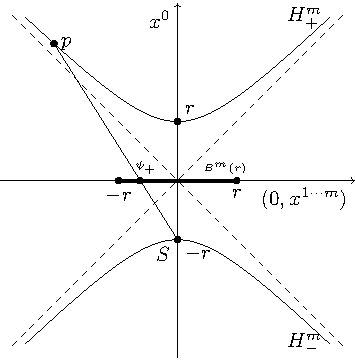
\includegraphics{fig/ch10-Hyperbolic.pdf}
    \caption{双曲空间}\label{chsm:pic_Hyperbolic}
\end{figure}

对任意$p=(x^0,x^1 ,\cdots,x^{m} )\in H^m_{+}(r)$(见图\ref{chsm:pic_Hyperbolic}),
连接点$p$和$S$的直线$l_{pS}$必定交超平面$x^{0}=0$于某点$\psi_{+}(p)$;很明显
交点$\psi_{+}(p)$位于$B^m(r)$内(不可能不与之相交);同时$\psi_{+}:H^m_{+}(r)\to B^m(r)$是双射.
对于任意的点$p$,下面我们来求$\psi_{+}(p)$的坐标$(\xi^1,\cdots,\xi^{m})$.

过两点(此处是$p$和$S$点)直线方程是(直线上点的坐标是$(\xi^0,\cdots,\xi^m)$)
\begin{equation}
    \frac{\xi^1-0}{x^1 -0} =\frac{\xi^2-0}{x^2 -0}=\cdots=
    \frac{\xi^m-0}{x^m -0} = \frac{\xi^{0}+r}{x^{0} +r}
\end{equation}
令上式中的$\xi^{0}=0$可得$\psi_{+}(p)$坐标如下
\begin{equation}
    (\xi^1,\cdots,\xi^m)=\psi_{+}(x^0,x^1 ,\cdots,x^{m})=
    \frac{r}{r+x^{0}}(x^1,\cdots,x^m).
\end{equation}
反之.将上式求平方和,并利用$\sum_{i=1}^{m}(x^i)^2 -(x^{0})^2=-r^2$,可得
\begin{align*}
    & \sum_{k=1}^{m}(\xi^k)^2=\frac{r^2 }{(r+x^{0})^2}\left(\sum_{i=1}^{m}(x^i)^2\right)
    =\frac{r^2 }{(r+x^{0})^2}\left(-r^2+(x^{0})^2\right) \\
    \Rightarrow \ 
    & x^{0} = \frac{r\left(r^2+\sum\nolimits_k(\xi^k)^2\right)}{r^2-\sum\nolimits_k(\xi^k)^2},
    {\quad \text{或} \quad } x^{0}= -r \ (\text{舍弃}) .
\end{align*}
有了$x^0$坐标表达式,其它坐标几乎一望而知,它们是
\begin{align}
    (x^{0},& x^1,\cdots,x^m) = \psi_{+}^{-1}(\xi^1,\cdots,\xi^m) \notag \\
    =&\frac{r}{r^2-\sum\nolimits_k(\xi^k)^2}
    \left(+r^2+\sum_{k=1}^m(\xi^k)^2, \ 2 r \xi^1, \cdots, \ 2 r \xi^m \right),
    \label{chdm:eqn_hybxi2x} \\
    (x^{0},& x^1,\cdots,x^m) = \psi_{-}^{-1}(\eta^1,\cdots,\eta^m) \notag \\
    =&\frac{r}{r^2-\sum\nolimits_k(\eta^k)^2}
    \left(- r^2-\sum_{k=1}^m (\eta^k)^2 , \ 2 r \eta^1, \cdots, \ 2 r \eta^m \right).
    \label{chdm:eqn_mybeta2x}
\end{align}
上面第二式为双曲空间下叶的坐标(其中$\eta^i=\frac{r x^i}{r-x^{0}}$),请读者补齐推导过程.
不难看出映射$\psi_{\pm}$及$\psi_{\pm}^{-1}$都是无穷阶可微函数,
所以$\psi_{\pm}:H^m_{\pm}(r)\to B^m(r)$是光滑同胚.

$\mathbb{R}^{m+1}_1$度规为广义Lorentz度规,即
\begin{equation*}
    g_{ab}X^a Y^b = \bigl(-({\rm d}x^0)_a({\rm d}x^0)_b+ \sum_{i=1}^{m}({\rm d}x^i)_a({\rm d}x^i)_b\bigr)
    X^a Y^b=-X^0 Y^0 + \sum_{i=1}^{m} X^i Y^i,
\end{equation*}
其中$X^a, Y^a\in \mathbb{R}^{m+1}$是任意矢量.显然,有
\begin{equation}
    g_{ab}X^a Y^b = \frac{1}{2}\bigl(g_{ab}(X+Y)^a(X+Y)^b -g_{ab}X^a X^b -g_{ab}Y^a Y^b\bigr).
\end{equation}
从上式可见,只需研究$g_{ab}X^a X^b$就可讨论整个Lorentz度规了.
在物理学中(见定义\ref{chrg:def_Minkowski-space}和\ref{chrg:def_vector-property}),
只讨论类时矢量和零模矢量,而它们正好与双曲空间有一一对应关系;类时矢量对应$r>0$,零模矢量对应$r=0$.
为简单起见,我们假设所有矢量的第零维分量是正的(指向未来),
同时只讨论类时矢量;这样只需讨论双曲空间的上叶即可.
从上面的讨论可以看出,类时矢量的Lorentz度规内积可以转化为双曲上叶中(这种转换是双射).

读者需要注意,我们只给$\mathbb{R}^{m+1}_1$选定了度规,还不知道$H^m_{\pm}(r)$或$B^m(r)$度规;
下面我们来计算它们的诱导度规.
很明显,包含映射$\imath :H^m_{+}(r) \to \mathbb{R}^{m+1}_1$是正则嵌入的;
令$\varphi=\imath \circ \psi_{+}^{-1}$,则由上面的讨论可知:$\varphi:B^m(r)\to \mathbb{R}^{m+1}_1$也是
光滑、正则嵌入映射;当然它们都是浸入的了.根据式\eqref{chsm:eqn_gijhab}可以求得$B^m(r)$的
诱导度规$h_{ab}=\varphi^{*} g_{ab}$,直接计算即可
\setlength{\mathindent}{0em}
\begin{equation}\label{chsm:eqn_gphiha}
    h_{ab}= \left(\sum_{\alpha=1}^{m}\frac{\partial x^\alpha}{\partial \xi^i}
    \frac{\partial x^\alpha}{\partial \xi^j} -\frac{\partial x^0}{\partial \xi^i}
    \frac{\partial x^0}{\partial \xi^j} \right)
    ({\rm d}\xi^i)_a ({\rm d}\xi^j)_b
    = \frac{4r^4 \sum\nolimits_{i=1}^{m} ({\rm d}\xi^i)_a ({\rm d}\xi^i)_b} 
    {(r^2-\sum\nolimits_{k=1}^{m} (\xi^k)^2)^2}.
\end{equation}\setlength{\mathindent}{2em}
可见这个度规是正定的,因而$B^m(r)$是一个正定黎曼流形.

还可以求得$H^m_{+}(r)$中的诱导度规$h'_{ab}=\imath ^* g_{ab}$
(假设$x^1,\cdots,x^m$是独立变量,$x^0$可由上述量来表示),
根据式\eqref{chsm:eqn_gijhab}经过计算可得
\begin{equation}\label{chsm:eqn_gphihabb}
    \begin{aligned}
        h'_{ab}=& \sum_{ij=1}^{m}\left(\sum_{\alpha,\beta=1}^{m}\frac{\partial x^\alpha}{\partial x^i}
        \frac{\partial x^\beta}{\partial x^j}\delta_{\alpha\beta} -\frac{\partial x^0}{\partial x^i}
        \frac{\partial x^0}{\partial x^j} \right)    ({\rm d} x^i)_a ({\rm d} x^j)_b  \\
        =& \sum_{ij=1}^{m}\left(\delta_{ij}-\frac{x^i x^j}{r^2+\sum_{k=1}^{m}(x^k)^2}\right)({\rm d} x^i)_a ({\rm d} x^j)_b \\
        \xlongequal{\ref{chdm:eqn_hybxi2x}}&
        \frac{4r^4 \sum\nolimits_{i=1}^{m} ({\rm d}\xi^i)_a ({\rm d}\xi^i)_b} {(r^2-\sum\nolimits_{k=1}^{m} (\xi^k)^2)^2}.
    \end{aligned}
\end{equation}
上式最后一步推导较为繁琐,计算冗长,所得结果与式\eqref{chsm:eqn_gphiha}相同.
这说明$(H^m_{+}(r),\imath ^* g_{ab})$和$(B^m(r),\varphi ^* g_{ab})$是等距同胚.

%推导过程
%\setlength{\mathindent}{0em}
%\begin{align*}
%    ({\rm d} x^i)_a =& \frac{2a^2 (r^2-\sum\nolimits_k(\xi^k)^2) ({\rm d} \xi^i)_a
    %    + 4a^2 \xi^i \sum\nolimits_l \xi^l ({\rm d} \xi^l)_a}{(r^2-\sum\nolimits_k(\xi^k)^2)^2}
%\end{align*}
%第一项
%\begin{align*}
%    &\sum_{ij=1}^{m}\delta_{ij}({\rm d} x^i)_a ({\rm d} x^j)_b = \sum_{i=1}^{m}({\rm d} x^i)_a ({\rm d} x^i)_b \\
%    =& \frac{2a^2 (r^2-\sum\nolimits_k(\xi^k)^2) ({\rm d} \xi^i)_a
    %        + 4a^2 \xi^i \sum\nolimits_l \xi^l ({\rm d} \xi^l)_a}{(r^2-\sum\nolimits_k(\xi^k)^2)^2}
%    \frac{2a^2 (r^2-\sum\nolimits_k(\xi^k)^2) ({\rm d} \xi^i)_b
    %        + 4a^2 \xi^i \sum\nolimits_l \xi^l ({\rm d} \xi^l)_b}{(r^2-\sum\nolimits_k(\xi^k)^2)^2} \\
%    =& \frac{1}{(r^2-\sum\nolimits_k(\xi^k)^2)^4} \biggl(
%    4a^4 (r^2-\sum\nolimits_k(\xi^k)^2)^2 \sum_{i=1}^{m} ({\rm d} \xi^i)_a ({\rm d} \xi^i)_b+
%    16a^4 (r^2-\sum\nolimits_k(\xi^k)^2)  \sum\nolimits_{il} \xi^l \xi^i  ({\rm d} \xi^i)_a ({\rm d} \xi^l)_b \\
%    & + 16a^4 \sum_{i=1}^{m} (\xi^i)^2 \sum\nolimits_{ln} \xi^l\xi^m ({\rm d} \xi^l)_a  ({\rm d} \xi^m)_b  \biggr) \\
%    =&\frac{1}{(r^2-\sum\nolimits_k(\xi^k)^2)^4} \biggl(
%    4a^4 (r^2-\sum\nolimits_k(\xi^k)^2)^2 \sum_{i=1}^{m} ({\rm d} \xi^i)_a ({\rm d} \xi^i)_b+
%    16a^6 \sum\nolimits_{ln} \xi^l \xi^m  ({\rm d} \xi^m)_a ({\rm d} \xi^l)_b  \biggr)
%\end{align*}
%第二项
%\begin{align*}
%    &\sum_{ij=1}^{m} x^i x^j ({\rm d} x^i)_a ({\rm d} x^j)_b
%    =\sum_{ij=1}^{m} \frac{4a^4 \xi^i \xi^j}{(r^2-\sum\nolimits_k(\xi^k)^2)^2}
%    \frac{2a^2 (r^2-\sum\nolimits_k(\xi^k)^2) ({\rm d} \xi^i)_a
    %        + 4a^2 \xi^i \sum\nolimits_l \xi^l ({\rm d} \xi^l)_a}{(r^2-\sum\nolimits_k(\xi^k)^2)^2} \\
%    &\times \frac{2a^2 (r^2-\sum\nolimits_k(\xi^k)^2) ({\rm d} \xi^j)_b
    %        + 4a^2 \xi^j \sum\nolimits_l \xi^l ({\rm d} \xi^l)_b}{(r^2-\sum\nolimits_k(\xi^k)^2)^2} \\
%    =& \frac{16a^8 }{(r^2-\sum\nolimits_k(\xi^k)^2)^6} \sum_{ij=1}^{m} \biggl(\xi^i \xi^j
%    \Bigl((r^2-\sum\nolimits_k(\xi^k)^2) ({\rm d} \xi^i)_a + 2 \xi^i \sum\nolimits_l \xi^l ({\rm d} \xi^l)_a\Bigr)
%    \Bigl((r^2-\sum\nolimits_k(\xi^k)^2) ({\rm d} \xi^j)_b + 2 \xi^j \sum\nolimits_n \xi^m ({\rm d} \xi^m)_b\Bigr)  \biggr) \\
%    =&\frac{16a^8 }{(r^2-\sum\nolimits_k(\xi^k)^2)^6} \biggl(
%    (r^2-\sum\nolimits_k(\xi^k)^2)^2  \sum_{ij=1}^{m} \xi^i \xi^j  ({\rm d} \xi^i)_a ({\rm d} \xi^j)_b
%     + 2(r^2-\sum\nolimits_k(\xi^k)^2) \Bigl(\sum_{j=1}^{m} (\xi^j)^2\Bigr)
%        \sum_{in=1}^{m} \xi^i\xi^m ({\rm d} \xi^i)_a ({\rm d} \xi^m)_b   \\
%    &+2 (r^2-\sum\nolimits_k(\xi^k)^2) \sum_{i=1}^{m}(\xi^i)^2
%     \sum\nolimits_{jl} \xi^l ({\rm d} \xi^l)_a \xi^j  ({\rm d} \xi^j)_b
%    + 4 \sum_{ij=1}^{m}(\xi^i)^2 (\xi^j)^2  \sum\nolimits_l \xi^l
%    ({\rm d} \xi^l)_a \sum\nolimits_n \xi^m ({\rm d} \xi^m)_b     \biggr) \\
%    =&\frac{16a^8 }{(r^2-\sum\nolimits_k(\xi^k)^2)^6} \biggl(
%    (r^2-\sum\nolimits_k(\xi^k)^2)^2
%    + 4(r^2-\sum\nolimits_k(\xi^k)^2) \Bigl(\sum_{j=1}^{m} (\xi^j)^2\Bigr)
%    + 4 \sum_{ij=1}^{m}(\xi^i)^2 (\xi^j)^2    \biggr)
%    \sum_{ln=1}^{m} \xi^l \xi^m  ({\rm d} \xi^l)_a ({\rm d} \xi^m)_b \\
%    =&\frac{16a^8 }{(r^2-\sum\nolimits_k(\xi^k)^2)^6} \biggl(
%    (r^2+\sum\nolimits_k(\xi^k)^2)^2   \biggr)
%    \sum_{ln=1}^{m} \xi^l \xi^m  ({\rm d} \xi^l)_a ({\rm d} \xi^m)_b
%\end{align*}
%而
%\begin{align*}
%    r^2+\sum_{k=1}^{m}(x^k)^2= r^2+
%    \sum_{i=1}^{m} \frac{4a^4 \xi^i \xi^i}{(r^2-\sum\nolimits_k(\xi^k)^2)^2}
%    =r^2 \frac{(r^2+\sum\nolimits_k(\xi^k)^2)^2}{(r^2-\sum\nolimits_k(\xi^k)^2)^2}
%\end{align*}
%综合以上三式,有
%\begin{align*}
%    &\frac{1}{(r^2-\sum\nolimits_k(\xi^k)^2)^4} \biggl(
%    4a^4 (r^2-\sum\nolimits_k(\xi^k)^2)^2 \sum_{i=1}^{m} ({\rm d} \xi^i)_a ({\rm d} \xi^i)_b+
%    16a^6 \sum\nolimits_{ln} \xi^l \xi^m  ({\rm d} \xi^m)_a ({\rm d} \xi^l)_b  \biggr) \\
%    &- \frac{16a^6 }{(r^2-\sum\nolimits_k(\xi^k)^2)^4}
%    \sum_{ln=1}^{m} \xi^l \xi^m  ({\rm d} \xi^l)_a ({\rm d} \xi^m)_b \\
%    =& \frac{ 4a^4 ({\rm d} \xi^i)_a ({\rm d} \xi^i)_b}{(r^2-\sum\nolimits_k(\xi^k)^2)^2}
%\end{align*}
%\setlength{\mathindent}{2em}

\begin{example}
    具体计算一例.当$m=1$时,设$v^a=v_{\xi}(\frac{\partial}{\partial \xi})^a\in T_pB^1(r)$,
    根据式\eqref{chsm:eqn_gphiha},有$h_{ab}v^a v^b= \frac{4r^4 v^2_\xi}{(r^2-\xi^2)^2}$;
    这是正定的.
    
    再计算Lorentz度规下的数值.推前$v^a$有$\varphi_*(v^a)= \frac{4r^3\xi v_\xi}{(r^2-\xi^2)^2}
    (\frac{\partial}{\partial x^0})^c+ \frac{2r^2(r^2+\xi^2) v_\xi}{(r^2-\xi^2)^2}(\frac{\partial}{\partial x^1})^c$;
    再来计算矢量长度,$g_{ab}v^a v^b= \frac{4r^4 v^2_\xi}{(r^2-\xi^2)^2}$;两者相等.
\end{example}



%\subsection{统一表示}
\paragraph{统一表示}
前面几节,我们把$\mathbb{R}^{m+1}_\nu$中的坐标(比如$x^0$)直接
用其它坐标($x^1,\cdots,x^m$)表示出来,
然后给出了伪球面、伪双曲面的度规;这种方式最为直接,但所得公式各不相同.
黎曼最早用同一公式表示了超球面和双曲空间的度规,之后被其他人推广到了伪球面、伪双曲面;
详见\S \ref{chhss:sec_SF} 定理\ref{chhss:thm_SRH-riemann}.




\section{超曲面四:相对论时空}\label{chsm:sec_3+1decomposition}
本节将光滑流形$(M,g)$的维数限定在四维,则超曲面$\Sigma$是三维的,度规$g$是Lorentz类型的($(-+++)$).
本小节拉丁字母表示$1,2,3$;希腊字母表示$0,1,2,3$.


流形$M$的切丛$TM$上存在一类时矢量场$(\frac{\partial }{\partial t})^a$,这一类时场将
流形$M$分解为一族类空超曲面$\{\Sigma_t\}$,整张超曲面$\Sigma_t$上的参数$t$是同一实数.
这族超曲面中任意两张不同参数的超曲面没有交集,即$\Sigma_t \cap \Sigma_{t'}=\varnothing,
\ \forall t \neq t' $.
流形$M$中任意一点都位于某张(且只在此张)$\Sigma_t$上,
即$\{\Sigma_t\}$能覆盖住流形$M$,$M=\bigcup_{t\in\mathbb{R}} \Sigma_t$.

从纯粹数学角度来看任意四维闵氏流形$(M,g)$,未必存在
这样的分解,或者说需要满足一定条件才存在这样的类时矢量场,然后依据这个
类时场将空间$M$划分成一族类空超曲面$\Sigma_t$;寻找数学上的这些存在性条件
(对物理学工作者来说)太过艰深.从物理学角度看,这样的分解一定存在,
因为我们就生活在这样的一个四维时空中,这个时空然后被$1+3$分解成时间和空间.



\index[physwords]{超曲面!ADM分解}
\index[physwords]{ADM分解}

\subsection{ADM分解}\label{chsm:sec_ADM}

类时场$(\frac{\partial }{\partial t})^a$自然是单参数的,参数是$t$;
我们约定它指向未来,即指向参数$t$增大的方向.
一般情形下,$(\frac{\partial }{\partial t})^a$未必与超曲面$\Sigma_t$处处正交;
假设类时矢量场$(\frac{\partial }{\partial t})^a$可分解为两个矢量场:
\begin{equation}\label{chsm:eqn_ADM}
    \left(\frac{\partial }{\partial t}\right)^a = N n^a + S^a .
\end{equation}
其中$n^a$是类空超曲面$\Sigma_t$的单位法矢量,所以有$n^a n_a =-1$;
标量场$N$称为\uwave{时移函数}(lapse function),
矢量场$S^a$称为\uwave{位移矢量场}(shift vector field),$S^a$切于类空超曲面$\Sigma_t$.
一般称这种分解方式为ADM分解\cite{ADM_2008}.很容易得到
\begin{equation*}
    ({\rm d}t)_a = -\frac{1}{N} n_a .\quad \text{因为}\
    1= ({\rm d}t)_a \left(\frac{\partial }{\partial t}\right)^a =
    -\frac{1}{N} n_a(N n^a + S^a)=-n_a n^a =1.
\end{equation*}

我们需要建立局部坐标系,类时矢量场$(\frac{\partial }{\partial t})^a$自然是
坐标基矢之一,它的积分曲线(见\S\ref{chdm:sec_One-Parameter-Transformations-Groups})是一条坐标线.
依据它分层的每张超曲面$\Sigma_t$都是三维类空曲面,在每张
超曲面上我们都选取三个线性无关的(即不在同一个二维超曲面内)类空矢量场;
当然可以选三个正交归一的类空矢量场,但目前暂不做此要求.
这四个坐标构成局部坐标系$\{x^0\equiv t,x^i \}$,基矢分别
是$\{(\frac{\partial }{\partial t})^a,(\frac{\partial }{\partial x^i})^a\}$.
类时矢量场$(\frac{\partial }{\partial t})^a$的积分曲线与每一个$\Sigma_t$都有且只有一个交点,
所有交点的三个类空坐标$\{x^i\}$自然取为相同的值;每张$\Sigma_t$上的参数$t$取同一值.

根据假设矢量场$S^a$是纯类空矢量场,切于$\Sigma_t$;而$n^a$正交于$\Sigma_t$,故有
\begin{equation}
    S^0 = S^a ({\rm d}t)_a= -\frac{1}{N} S^a n_a =0.
\end{equation}
因此
\begin{equation}
    S^a = \sum_{i=1}^{3} S^i \left(\frac{\partial }{\partial x^i}\right) ^a .
\end{equation}
令$S_a = g_{ab} S^b$,$S_i = S_a (\frac{\partial }{\partial x^i}) ^a$.

经计算可得度规场$g_{ab}$在局部坐标系$\{x^0\equiv t,x^i \}$的分量表达式:
\begin{small}
\begin{equation}\label{chsm:eqn_ADM-metric}
    g_{\mu\nu}=\begin{pmatrix}
        S^i S_i -N^2 & S_1 & S_2 &S_3 \\
        S_1 &g_{11} & g_{12} & g_{13} \\
        S_2 &g_{21} & g_{22} & g_{23} \\
        S_3 &g_{31} & g_{32} & g_{33}
    \end{pmatrix}, \
    g^{\mu\nu}=\frac{1}{N^{2}} \begin{pmatrix}
        -1 & S^1 & S^2 & S^3 \\
        S^1 & &  &  \\
        S^2 &N^{2} h_{ij}^{-1} & - & S^i S^j \\
        S^3 & &  &
    \end{pmatrix} .
\end{equation}
\end{small}
记$g_{ij}\equiv h_{ij},\ 1\leqslant i,j \leqslant 3$.
其中共轭度规右下角$3\times 3$的矩阵元是$g^{ij}= h_{ij}^{-1}-N^{-2}S^i S^j$,
其中$h_{ij}^{-1}$是指度规右下角$3\times 3$的矩阵$(g_{ij})$的逆;
需要注意的是矩阵外面还有一个因子.

可求得单位法矢量在$\{t,x^i\}$的分量表达式
\begin{equation}\label{chsm:eqn_ADM-n}
    n^a = \frac{1}{N} \left(\frac{\partial }{\partial t}\right)^a
    -\frac{S^i}{N} \left(\frac{\partial }{\partial x^i}\right)^a  ;\qquad
    n_a = -N ({\rm d}t)_a = -N \nabla_a t .
\end{equation}


诱导度规$h_{ab}=g_{ab}+n_a n_b$在$\{t,x^i\}$的分量表达式为
\begin{small}
\begin{subequations}\label{chsm:eqn_ADM-hab}
\begin{align}
    h_a^b =& \left( ({\rm d}x^i)_a +S^i ({\rm d}t)_a \right) 
    \left(\frac{\partial }{\partial x^i}\right)^b , \label{chsm:eqn_ADM-hab-1}\\
    h_{ab}=& S_k S^k ({\rm d}t)_a ({\rm d}t)_b + S_i\left( ({\rm d}t)_a ({\rm d}x^i)_b
    + ({\rm d}t)_b ({\rm d}x^i)_a \right) + g_{ij} ({\rm d}x^i)_a ({\rm d}x^j)_b .
    \label{chsm:eqn_ADM-hab-2} 
\end{align}
\end{subequations}
\end{small}
直接计算便可得到$\det(h_{\mu\nu})=0$,但$h=\det(h_{ij})\neq 0$.
且有$g=\det(g_{\mu\nu})=-N^2 \det(g_{ij})=-N^2 \det(h_{ij})$.
从而可以得到四维流形$M$体积元与三维超曲面$\Sigma_t$的诱导体积元之间的关系:
\begin{small}
\begin{equation}
   n^a \bigl(\sqrt{-g}({\rm d}x^0)_a \wedge ({\rm d}x^1)_b \wedge({\rm d}x^2)_c \wedge({\rm d}x^3)_d \bigr) 
        = N \sqrt{h} ({\rm d}x^1)_b \wedge({\rm d}x^2)_c \wedge({\rm d}x^3)_d  .
\end{equation}
\end{small}

虽然三维流形$\Sigma_t$上的度规场$h_{ij}\equiv g_{ij}$,
但是,从式\eqref{chsm:eqn_ADM-metric}可以看到一般情形下$h^{ij}=h_{ij}^{-1}\neq g^{ij}$,
而是$g^{ij}=h_{ij}^{-1} - S^i S^j/N^2$.



\index[physwords]{超曲面!时间导数}

\subsection{时间导数}

在适配坐标系中(见式\eqref{chdm:eqn_LieD-adaptedX}),李导数化为偏导数;
ADM分解后的坐标系就是一个适配坐标系,所有张量分量对参数$t$的偏导数都可以化作李导数.
在ADM分解中,参量$t$可以看作“时间”;故
张量场对切矢量场$(\frac{\partial }{\partial t})^a$的李导数可以看作对时间$t$的导数.

类空张量场$T^{a\cdots}_{b\cdots}\in \mathfrak{T}^p_q(\Sigma_t)$的李导数未必仍是类空张量场,
我们给其增加数次投影,这样的李导数自然仍是类空张量场.
\begin{equation}
    \dot{T}^{a\cdots}_{b\cdots} \equiv \widetilde{\Lie}_{\partial_t}{T}^{a\cdots}_{b\cdots}
    \overset{def}{=} h^a_{a'}\cdots h^{b'}_{b}\cdots {\Lie}_{\partial_t}{T}^{a'\cdots}_{b'\cdots} .
\end{equation}
$\widetilde{\Lie}_X$表示增加数次投影的${\Lie}_X$.
可以证明如下重要公式:
\begin{equation}\label{chsm:eqn_Lie-t-T}
    \widetilde{\Lie}_{\partial_t}{T}^{a\cdots}_{b\cdots}
    = \widetilde{\Lie}_{N n}{T}^{a\cdots}_{b\cdots}
     +\widetilde{\Lie}_{\vec{S}}{T}^{a\cdots}_{b\cdots}
    = N \widetilde{\Lie}_{n}{T}^{a\cdots}_{b\cdots}
    +\widetilde{\Lie}_{\vec{S}}{T}^{a\cdots}_{b\cdots} ,
    \quad \forall T^{a\cdots}_{b\cdots}\in \mathfrak{T}^p_q(\Sigma_t).
\end{equation}
由于$S^a$在ADM分解下是纯类空矢量场,在李导数的角标中,将其记为$\vec{S}$.
式$\widetilde{\Lie}_{Nn}{T}^a_{\cdot b}=N\widetilde{\Lie}_{n}{T}^{a\cdots}_{b\cdots}$的证明
较为繁琐,需先后计算$\widetilde{\Lie}_{Nn}{T}^{a\cdots}_{b\cdots}$
和$\widetilde{\Lie}_{n}{T}^{a\cdots}_{b\cdots}$,
然后即可验证它们相等.有了此等式,也就证明了式\eqref{chsm:eqn_Lie-t-T}.

%首先,经过较为冗长的推演可以证明
%\begin{align*}
%    \widetilde{\Lie}_{n}{T}^a_{\cdot b} = &
%    h^a_{a'} h^{b'}_{b} \left( n^e\nabla_e T^{a'}_{\cdot b'}
%    - T^{e}_{\cdot b'} \nabla_e n^{a'} + T^{a'}_{\cdot e} \nabla_{b'} n^e \right) \\
%    = &  (g^a_{a'} g^{b'}_{b} +n^a n_{a'}g^{b'}_{b}+ g^a_{a'} n^{b'}n_{b} + n^a n_{a'}n^{b'}n_{b})
%    \left(N n^e\nabla_e T^{a'}_{\cdot b'}
%    - T^{e}_{\cdot b'} \nabla_e n^{a'} + T^{a'}_{\cdot e} \nabla_{b'} n^e \right) \\
%    = &  g^a_{a'} g^{b'}_{b}   \left( n^e\nabla_e T^{a'}_{\cdot b'}
%    - T^{e}_{\cdot b'} \nabla_e n^{a'} + T^{a'}_{\cdot e} \nabla_{b'} n^e \right) \\
%    &+  n^a n_{a'}g^{b'}_{b}  \left( n^e\nabla_e T^{a'}_{\cdot b'}
%    - T^{e}_{\cdot b'} \nabla_e n^{a'} + \cancel{T^{a'}_{\cdot e} \nabla_{b'} n^e} \right) \\
%    &+ g^a_{a'} n^{b'}n_{b}    \left( n^e\nabla_e T^{a'}_{\cdot b'}
%    -\cancel{ T^{e}_{\cdot b'} \nabla_e n^{a'}}+ T^{a'}_{\cdot e} \nabla_{b'} n^e \right) \\
%    &+ n^a n_{a'}n^{b'}n_{b} \left( n^e\nabla_e T^{a'}_{\cdot b'}
%    -\cancel{ T^{e}_{\cdot b'} \nabla_e n^{a'}} + \cancel{T^{a'}_{\cdot e} \nabla_{b'} n^e} \right) \\
%    = &  n^e\nabla_e T^{a}_{\cdot b}
%    - T^{e}_{\cdot b} \nabla_e n^{a} + T^{a}_{\cdot e} \nabla_{b} n^e  \\
%    &+  n^a n_{a'}  \left( n^e\nabla_e T^{a'}_{\cdot b}
%    - T^{e}_{\cdot b} \nabla_e n^{a'}  \right) \\
%    &+  n^{b'}n_{b}    \left( n^e\nabla_e T^{a}_{\cdot b'}
%    + T^{a}_{\cdot e} \nabla_{b'} n^e \right) \\
%    &+ n^a n_{a'}n^{b'}n_{b}  n^e\nabla_e T^{a'}_{\cdot b'}  \\
%    = &  n^e\nabla_e T^{a}_{\cdot b}
%    - T^{e}_{\cdot b} \nabla_e n^{a} + T^{a}_{\cdot e} \nabla_{b} n^e  \\
%    &+  n^a n_{a'} n^e\nabla_e T^{a'}_{\cdot b}
%    -   \cancel{n^a n_{a'} T^{e}_{\cdot b} \nabla_e n^{a'}  } \\
%    &+  n^{b'}n_{b}  n^e\nabla_e T^{a}_{\cdot b'}
%    + n^{b'}n_{b} T^{a}_{\cdot e} \nabla_{b'} n^e \\
%    &- \cancel{n^a n_{a'} n_{b} T^{a'}_{\cdot b'} n^e\nabla_e n^{b'} } \\
%    = &  n^e\nabla_e T^{a}_{\cdot b}
%    - T^{e}_{\cdot b} \nabla_e n^{a} + T^{a}_{\cdot e} \nabla_{b} n^e
%    + n^a n_{c} n^e\nabla_e T^{c}_{\cdot b}
%    + n^{c}n_{b}  n^e\nabla_e T^{a}_{\cdot c}
%    + n^{c}n_{b} T^{a}_{\cdot e} \nabla_{c} n^e \\
%        = &  n^e\nabla_e T^{a}_{\cdot b}
%    - T^{e}_{\cdot b} \nabla_e n^{a} + T^{a}_{\cdot e} \nabla_{b} n^e
%    + n^a n_{c} n^e\nabla_e T^{c}_{\cdot b}
%    + {\color{red}n^cn_{b} n^{e} \nabla_c T^{a}_{\cdot e}
%    - n^{c}n_{b} n^e \nabla_{c}  T^{a}_{\cdot e}} \\
%    = &  n^e\nabla_e T^{a}_{\cdot b}
%    - T^{e}_{\cdot b} \nabla_e n^{a} + T^{a}_{\cdot e} \nabla_{b} n^e
%    + n^a n_{c} n^e\nabla_e T^{c}_{\cdot b}
%\end{align*}
%容易验证
%$n^b \widetilde{\Lie}_{n}{T}^a_{\cdot b} =0=n_a \widetilde{\Lie}_{n}{T}^a_{\cdot b}$.
%接着计算,
%\begin{align*}
%    \widetilde{\Lie}_{N n}{T}^a_{\cdot b} = &
%    h^a_{a'} h^{b'}_{b} \left(N n^e\nabla_e T^{a'}_{\cdot b'}
%    - T^{e}_{\cdot b'} \nabla_e (Nn^{a'}) + T^{a'}_{\cdot e} \nabla_{b'} (Nn^e) \right) \\
%    = &  (g^a_{a'} g^{b'}_{b} +n^a n_{a'}g^{b'}_{b}+ g^a_{a'} n^{b'}n_{b} + n^a n_{a'}n^{b'}n_{b})
%      \left(N n^e\nabla_e T^{a'}_{\cdot b'}
%      - T^{e}_{\cdot b'} \nabla_e (Nn^{a'}) + T^{a'}_{\cdot e} \nabla_{b'} (Nn^e) \right) \\
%    = &  g^a_{a'} g^{b'}_{b}   \left(N n^e\nabla_e T^{a'}_{\cdot b'}
%      - T^{e}_{\cdot b'} \nabla_e (Nn^{a'}) + T^{a'}_{\cdot e} \nabla_{b'} (Nn^e) \right) \\
%     &+  n^a n_{a'}g^{b'}_{b}  \left(N n^e\nabla_e T^{a'}_{\cdot b'}
%      - T^{e}_{\cdot b'} \nabla_e (Nn^{a'}) + T^{a'}_{\cdot e} \nabla_{b'} (Nn^e) \right) \\
%     &+ g^a_{a'} n^{b'}n_{b}    \left(N n^e\nabla_e T^{a'}_{\cdot b'}
%      - T^{e}_{\cdot b'} \nabla_e (Nn^{a'}) + T^{a'}_{\cdot e} \nabla_{b'} (Nn^e) \right) \\
%     &+ n^a n_{a'}n^{b'}n_{b} \left(N n^e\nabla_e T^{a'}_{\cdot b'}
%      - T^{e}_{\cdot b'} \nabla_e (Nn^{a'}) + T^{a'}_{\cdot e} \nabla_{b'} (Nn^e) \right) \\
%    =&    N n^e\nabla_e T^{a}_{\cdot b}
%    - T^{e}_{\cdot b} n^{a} \nabla_e N - T^{e}_{\cdot b} N  \nabla_e n^a
%    + \cancel{T^{a}_{\cdot e} n^e \nabla_{b} N} + T^{a}_{\cdot e} N  \nabla_b n^e  \\
%    &+  n^a n_{a'} \left(N n^e\nabla_e T^{a'}_{\cdot b}
%    - T^{e}_{\cdot b} \nabla_e (Nn^{a'}) +\cancel{ T^{a'}_{\cdot e} \nabla_{b} (Nn^e)} \right) \\
%    &+  n^{b'}n_{b}    \left(N n^e\nabla_e T^{a}_{\cdot b'}
%    -\cancel{ T^{e}_{\cdot b'} \nabla_e (Nn^{a})} + T^{a}_{\cdot e} \nabla_{b'} (Nn^e) \right) \\
%    &+ n^a n_{a'}n^{b'}n_{b} \left(N n^e\nabla_e T^{a'}_{\cdot b'}
%    - \cancel{T^{e}_{\cdot b'} \nabla_e (Nn^{a'})} + \cancel{T^{a'}_{\cdot e} \nabla_{b'} (Nn^e)} \right) \\
%    =&    N n^e\nabla_e T^{a}_{\cdot b}
%    - T^{e}_{\cdot b} n^{a} \nabla_e N - T^{e}_{\cdot b} N  \nabla_e n^a
%    + T^{a}_{\cdot e} N  \nabla_b n^e  \\
%    &+  n^a n_{a'} \left(N n^e\nabla_e T^{a'}_{\cdot b}
%    - T^{e}_{\cdot b} n^{a'} \nabla_e N - T^{e}_{\cdot b} N \nabla_e  n^{a'} \right) \\
%    &+  n^{b'}n_{b}    \left(N n^e\nabla_e T^{a}_{\cdot b'}
%    + T^{a}_{\cdot e} n^e\nabla_{b'} N + T^{a}_{\cdot e}N \nabla_{b'} n^e \right) \\
%    &+ n^a n_{a'}n^{b'}n_{b} \left(N n^e\nabla_e T^{a'}_{\cdot b'}   \right) \\
%    =&      N n^e\nabla_e T^{a}_{\cdot b}
%    - {\color{red}T^{e}_{\cdot b} n^{a} \nabla_e N }
%    - T^{e}_{\cdot b} N  \nabla_e n^a + T^{a}_{\cdot e} N  \nabla_b n^e  \\
%    &+  N n^a n_{a'} n^e\nabla_e T^{a'}_{\cdot b}
%     + {\color{red} n^a T^{e}_{\cdot b} \nabla_e N }
%     - {\cancel{n^a n_{a'}T^{e}_{\cdot b} N \nabla_e  n^{a'}}} \\
%    &+  n^{b'}n_{b} N n^e\nabla_e T^{a}_{\cdot b'}
%    + {\cancel{n^{b'}n_{b}T^{a}_{\cdot e} n^e\nabla_{b'} N}}
%    + n^{b'}n_{b}T^{a}_{\cdot e}N \nabla_{b'} n^e  \\
%    &+ n^a n_{a'}n^{b'}n_{b} N n^e\nabla_e T^{a'}_{\cdot b'}    \\
%    =&    N n^e\nabla_e T^{a}_{\cdot b}
%    - T^{e}_{\cdot b} N  \nabla_e n^a + T^{a}_{\cdot e} N  \nabla_b n^e
%    + n^{b'}n_{b}T^{a}_{\cdot e}N \nabla_{b'} n^e  \\
%    &+  N n^a n_{a'} n^e\nabla_e T^{a'}_{\cdot b}
%    +  n^{b'}n_{b} N n^e\nabla_e T^{a}_{\cdot b'}
%    + n^a n_{a'}n^{b'}n_{b} N n^e\nabla_e T^{a'}_{\cdot b'}    \\
%     =&    N n^e\nabla_e T^{a}_{\cdot b}
%    - T^{e}_{\cdot b} N  \nabla_e n^a + T^{a}_{\cdot e} N  \nabla_b n^e
%    +  {\color{red}n^{b'}n_{b}T^{a}_{\cdot e}N \nabla_{b'} n^e} \\
%    &-  N n^a T^{a'}_{\cdot b} n^e\nabla_e  n_{a'}
%    -  {\color{red}N n_{b} T^{a}_{\cdot b'}  n^e\nabla_e n^{b'}}
%    - {\cancel{N n^a n_{a'}n_{b} T^{a'}_{\cdot b'} n^e\nabla_e n^{b'}  }}  \\
%    =& N n^e\nabla_e T^{a}_{\cdot b}
%    - T^{e}_{\cdot b} N  \nabla_e n^a + T^{a}_{\cdot e} N  \nabla_b n^e
%    -  N n^a T^{a'}_{\cdot b} n^e\nabla_e  n_{a'}\\
%   =& N \left(n^e\nabla_e T^{a}_{\cdot b} - T^{e}_{\cdot b}  \nabla_e n^a + T^{a}_{\cdot e}  \nabla_b n^e
%      +  n^a  n_{c} n^e\nabla_e T^{c}_{\cdot b} \right)
%\end{align*}

%式\eqref{chsm:eqn_Lie-t-T}可以推广到任意$\Tpq{p}{q}$型张量场.


我们来计算超曲面上两个最基本张量的时间导数.
首先是诱导度规$h_{ab}$
\begin{equation}\label{chsm:eqn_Lie-t-hab}
    \dot{h}_{ab} = N \widetilde{\Lie}_{n}{h}_{ab}
    +\widetilde{\Lie}_{\vec{S}}{h}_{ab}
    \xlongequal{\ref{chsm:eqn_Kab-2}}
    -2N K_{ab}
    +\widetilde{\Lie}_{\vec{S}}{h}_{ab} .
\end{equation}
其次是外曲率$K_{ab}$的时间导数为:
\setlength{\mathindent}{0em}
\begin{equation}\label{chsm:eqn_Lie-t-Kab}
    \dot{K}_{ab} = -{}^4 R_{cd} N h^c_a h^d_b + {}^3 R_{ab} N - 2N K^c_a K_{cb}
     + N K K_{ab} - {\rm D}_a {\rm D}_b N +\widetilde{\Lie}_{\vec{S}}{K}_{ab}.
\end{equation}\setlength{\mathindent}{2em}
证明此式需分为两步.第一步,我们定义{\heiti 单位法矢量$n^a$的四加速度}:
\begin{equation}\label{chsm:eqn_Acceleration}
    A_a \overset{def}{=} n^b \nabla_b n_a =N^{-1} {\rm D}_a N .
\end{equation}
注意到明显有:$n^a A_a =0 $.上式最后一步的计算过程是:  %\setlength{\mathindent}{0em}
\begin{align*}
    A_a =& n^b \nabla_b n_a = -n^b\nabla_b ( N \nabla_a t )
    = -(n^b\nabla_b  N) \nabla_a t  -  N n^b\nabla_b  \nabla_a t \\
    =& (n^b\nabla_b  N) \frac{n_a}{N} -  N n^b\nabla_a  \nabla_b t 
    = n_a \frac{1}{N} n^b\nabla_b N   +  N n^b\nabla_a  \frac{n_b}{N}  \\
    =& n_a \frac{1}{N} n^b\nabla_b N + N n^b n_b \nabla_a \frac{1}{N} 
    +  \frac{N}{2N} {\cancel{\nabla_a  (n_bn^b)}} \\
    =& N^{-1} n_a n^b\nabla_b N + N^{-1} \nabla_a N
    = N^{-1} (n_a n^b + \delta^b_a )\nabla_b N
    =N^{-1} {\rm D}_a N .
\end{align*} %\setlength{\mathindent}{2em}
第二步,因$\dot{K}_{ab} = N \widetilde{\Lie}_{n}{K}_{ab} +\widetilde{\Lie}_{\vec{S}}{K}_{ab}$,
故只需计算$\widetilde{\Lie}_{n}{K}_{ab}$即可.
\begin{align*}
    -\widetilde{\Lie}_{n} K_{ab} =& -
     h_a^{c} h^{d}_{b} \left( n^e\nabla_e K_{cd}
     + K_{ed} \nabla_{c} n^e + K_{ce} \nabla_{d} n^e \right) \\
     =&  h_a^{c} h^{d}_{b} \bigl( n^e\nabla_e ( \nabla_{c} n_{d} + n_{c} A_{d} )
       + K_{ed} (K_c^e + n_c A^e) + K_{ce} (K_d^e +n_d A^e) \bigr) \\
%     =&  h_a^{c} h^{d}_{b} \bigl( n^e \nabla_e  \nabla_{c} n_{d}
%      + n^e n_{c} \nabla_e A_{d}  + A_{d}  n^e\nabla_e n_{c}  \\
%     &+ K_{ed} K_c^e + n_c K_{ed} A^e + K_{ce} K_d^e +n_d K_{ce}A^e \bigr) \\
     =&  h_a^{c} h^{d}_{b} \bigl( n^e (\nabla_c  \nabla_e n_{d} - {}^4R_{fdec}n^f)
     + \cancel{n^e n_{c} \nabla_e A_{d}}  - A_{d}  n^e (\cancel{K_{ec}}+n_e A_c)  \\
     & + 2K_{ed} K_c^e + \cancel{n_c K_{ed} A^e} + \cancel{n_d K_{ce}A^e} \bigr)
        \quad \text{其中} n^e K_{ec}=0,\  h_a^{c}n_c=0= h^{d}_{b} n_d \\
     =&  h_a^{c} h^{d}_{b} \bigl(   \nabla_c (n^e \nabla_e n_{d})- (\nabla_cn^e)  \nabla_e n_{d}
      - {}^4R_{fdec}n^f n^e  +  A_d A_c  + 2K_{ed} K_c^e  \bigr) \\
%     =&  h_a^{c} h^{d}_{b} \bigl(   \nabla_c A_{d}
%     - (K_c^e + \cancel{n_c A^e} )(K_{ed} + \cancel{n_e A_d})  - {}^4R_{fdec}n^f n^e
%      + A_d A_c  + 2K_{ed} K_c^e  \bigr) \\
     =&  h_a^{c} h^{d}_{b} \bigl(   \nabla_c A_{d}
      - {}^4R_{fdec}n^f n^e
      + A_d A_c  + K_{ed} K_c^e  \bigr) \\
      \xlongequal{\ref{chsm:eqn_contractRicci}}&
      h_a^{c} h^{d}_{b} \bigl(   \nabla_c A_{d}
      + A_d A_c  + K_{ed} K_c^e  \bigr)
      +{}^{4} {R}_{ef} h^f_a h^e_b - {}^{3}{R}_{ab}
      - K_{ab}K + K_{b}^e K_{ea}   \\
%      =&  {\rm D}_a A_{b}  + A_a A_b  + K_{eb} K_a^e
%      +{}^{4} {R}_{ef} h^f_a h^e_b - {}^{3}{R}_{ab}
%      - K_{ab}K + K_{b}^e K_{ea}   \\
      =&  {\rm D}_a (N^{-1}{\rm D}_b N)  + A_a A_b
      +{}^{4} {R}_{ef} h^f_a h^e_b - {}^{3}{R}_{ab}
      - K_{ab}K +2 K_{b}^e K_{ea}   \\
%      =&  N^{-1}{\rm D}_a {\rm D}_b N +({\rm D}_b N) (- N ^{-2}{\rm D}_a N) + A_a A_b
%      +{}^{4} {R}_{ef} h^f_a h^e_b - {}^{3}{R}_{ab}
%      - K_{ab}K +2 K_{b}^e K_{ea}   \\
      =&  N^{-1}{\rm D}_a {\rm D}_b N
      +{}^{4} {R}_{ef} h^f_a h^e_b - {}^{3}{R}_{ab}
      - K_{ab}K +2 K_{b}^e K_{ea} .
\end{align*}
将上式带回,即可证明式\eqref{chsm:eqn_Lie-t-Kab}.

%用$h^c_d h^a_b$缩并式\eqref{chsm:eqn_contractRicci}两端
%\begin{align*}
%    {}^{3}{R}_{ac} h^c_d h^a_b =&{}^{4} {R}_{ac}h^c_d h^a_b
%    -{}^{4}{R}_{ec} {n}_{a} {n}^{e} h^c_d h^a_b\epsilon
%    -{}^{4}{R}_{af} {n}_{c} {n}^{f} h^c_d h^a_b \epsilon
%    +{}^{4}{R}_{ef} {n}_{a} {n}_{c} {n}^{e} {n}^{f} h^c_d h^a_b  \\
%    &- {}^{4}{R}_{aecf} {n}^{e} {n}^{f} h^c_d h^a_b \epsilon
%    +\epsilon (K_{ac}K - K_{a}^e K_{ec} ) h^c_d h^a_b
%    \quad \Rightarrow \\
%    {}^{3}{R}_{bd}  =&{}^{4} {R}_{ac}h^c_d h^a_b
%     + {}^{4}{R}_{aecf} {n}^{e} {n}^{f} h^c_d h^a_b
%     - (K_{bd}K - K_{b}^e K_{ed} )
%         \quad \Rightarrow \\
%     {}^{3}{R}_{ab}  =&{}^{4} {R}_{ef} h^f_a h^e_b
%     + {}^{4}{R}_{decf} {n}^{e} {n}^{f} h^c_a h^d_b
%     - K_{ab}K + K_{b}^e K_{ea}
%\end{align*}















\section*{小结}
本章主要参考了\parencite{chen-li-2023-2ed-v1,oneill1983}相应章节.




\printbibliography[heading=subbibliography,title=第\ref{chsm}章参考文献]

\endinput
